%%% 华中科技大学硕士学位论文 - 基于驱动程序替换的物联网设备固件仿真技术研究
%%% Local Variables:
%%% mode: Xelatex
%%% TeX-master: t
%%% End:

\documentclass[finalformat,mathCMR,redheader]{HUSTthesis}

\raggedbottom

\usepackage{HUSTtils}
\usepackage{pgfplots}
\pgfplotsset{compat=1.18}
\usepgfplotslibrary{groupplots}
\renewcommand{\lstlistingname}{代码清单}
\lstdefinestyle{Python}{
  language=Python,
  backgroundcolor=\color{backgroundColour},
  commentstyle=\color{mGreen},
  keywordstyle=\color{magenta},
  basicstyle=\ttfamily\scriptsize\bfseries,
  columns=fullflexible,
  breaklines=true,
  breakatwhitespace=true,
  showstringspaces=false,
  keepspaces=true,
  numbers=left,
  numbersep=5pt,
  showspaces=false,
  showtabs=false,
  tabsize=2
}

\lstdefinelanguage{CodeQL}{
  morekeywords={
    import, from, where, select,
    exists, predicate, class, module,
    and, or, not, true, false, instanceof
  },
  sensitive=true,
  morecomment=[l]{//},
  morecomment=[s]{/*}{*/},
  morestring=[b]"
}

\lstdefinestyle{CodeQL}{
  backgroundcolor=\color{backgroundColour},
  commentstyle=\color{mGreen},
  keywordstyle=\color{magenta},
  basicstyle=\ttfamily\scriptsize\bfseries,
  breaklines=true,
  captionpos=b,
  keepspaces=true,
  numbers=left,
  numbersep=5pt,
  showspaces=false,
  showstringspaces=false,
  showtabs=false,
  tabsize=2,
  language=CodeQL
}
\setmainfont{Times New Roman}

\begin{document}

%定义所有的eps文件在 figures 子目录下
\graphicspath{{figures/}}

% 生成封面，版权页，摘要
\frontmatter
% 论文基本信息
\ctitle{基于驱动程序替换的物联网设备固件仿真技术研究}
\etitle{Research on IoT Device Firmware Emulation Technology Based on Driver Replacement}

% 中文摘要
\cabstract{
随着物联网技术的快速发展，物联网设备数量呈现爆炸式增长，其固件安全问题日益突出。固件仿真技术是进行固件安全测试和漏洞挖掘的重要手段，然而现有的固件仿真方法存在外设建模成本高、硬件依赖强、自动化程度不足等问题。传统的基于硬件建模的方法需要为每种外设手动建立仿真模型，工作量大且难以覆盖多样化的硬件生态；基于驱动层替换的方法虽然避免了底层硬件建模，但驱动函数的定位与替换仍高度依赖人工干预，难以实现规模化应用。

针对上述问题，本文提出一种结合大语言模型的自动化固件仿真方法。该方法通过静态分析识别固件中的硬件依赖代码，利用大语言模型生成可替代的驱动实现，并通过动态测试反馈闭环迭代优化仿真质量，从而在无需手动建立外设模型的情况下支持固件稳定运行。围绕该方法，本文主要开展三方面工作。首先，设计并实现硬件依赖代码自动识别模块，从驱动程序源码中提取硬件相关函数调用点、外设寄存器访问模式和驱动函数边界，构建可查询的驱动知识库。其次，构建基于大语言模型的驱动函数分析与替换模块，结合结构化提示词模板和函数分类策略生成替代代码，并通过编译修复循环提升代码可编译性。最后，引入动态测试反馈闭环机制，在固件运行异常时自动分析原因并反馈至替换模块，通过"生成—测试—反馈—修正"流程持续优化仿真质量。

实验结果表明：在35个测试固件上，系统共识别4029个驱动函数并生成1563个替换实现。与现有代表性方法相比，本文方法的平均人工介入时长为0.6小时/固件，体现出较低的人力依赖和较高的自动化程度。上述结果说明本文方法可支持STM32、NXP、Atmel三类平台及FreeRTOS、RT-Thread、Zephyr、裸机等系统环境下的固件仿真，并在给定实验设置下具备较好的工程实用价值。
}

% 中文关键词
\ckeywords{物联网安全；固件仿真；驱动程序替换；大语言模型；静态分析}

% 英文摘要
\eabstract{
With the rapid development of Internet of Things (IoT) technologies, the number of IoT devices has grown explosively, and firmware security issues have become increasingly prominent. Firmware emulation is an important approach for firmware security testing and vulnerability discovery. However, existing firmware emulation methods still face major challenges, including high peripheral modeling cost, strong hardware dependence, and limited automation. Traditional hardware-modeling methods require manually constructing an emulation model for each peripheral, which is labor-intensive and difficult to scale to diverse hardware ecosystems. Although driver-layer replacement methods avoid low-level hardware modeling, driver-function identification and replacement still rely heavily on manual effort, limiting large-scale application.

To address these issues, this paper proposes an automated firmware emulation method enhanced by large language models (LLMs). The method identifies hardware-dependent firmware code through static analysis, generates alternative driver implementations with LLMs, and iteratively improves emulation quality through a dynamic testing feedback loop, thereby enabling stable firmware execution without manual peripheral modeling. Based on this method, this work makes three main contributions. First, it designs and implements an automatic hardware-dependency identification module that extracts hardware-related function call sites, peripheral register access patterns, and driver-function boundaries to build a queryable driver knowledge base. Second, it develops an LLM-based driver-function analysis and replacement module that combines structured prompts and function-classification strategies to generate replacement code and improve compilability through a compile-repair loop. Third, it introduces a dynamic testing feedback loop that analyzes runtime failures and feeds diagnostics back to the replacement module, continuously improving emulation quality through a "generate-test-feedback-revise" cycle.

Experimental results show that, across 35 firmware samples, the system identified 4,029 driver functions and generated 1,563 replacement implementations. Compared with representative baseline methods, the average manual intervention time was 0.6 hours per firmware, indicating lower human dependence and a higher degree of automation. These results indicate that the proposed method supports firmware emulation across STM32, NXP, and Atmel platforms, as well as FreeRTOS, RT-Thread, Zephyr, and bare-metal environments, and demonstrates practical engineering value under the given experimental setup.
}

% 英文关键词
\ekeywords{IoT Security; Firmware Emulation; Driver Replacement; Large Language Model; Static Analysis}

\makecover

%目录
\tableofcontents

\mainmatter
\chapter{绪论}
\label{chap:intro}

\section{研究背景与意义}
\label{sec:bg}

近年来，随着物联网（Internet of Things, IoT）技术迅速发展，物联网设备已被广泛用于智能家居、智慧城市、新能源、车联网、医疗健康等多个应用领域。根据 GSMA 发布的《The mobile economy 2020》报告显示，2019 年全球物联网总连接数达到 120 亿，预计到 2025 年，全球物联网总连接数规模将达到 246 亿，年复合增长率高达 13\%\cite{gsma2020mobile}。物联网操作系统是一种面向物联网设备和应用的轻量级嵌入式操作系统，它可以提供更好的设备管理、数据处理和安全性能。目前，市场上有许多物联网操作系统，例如华为的 OpenHarmony\cite{openharmony}、亚马逊的 FreeRTOS\cite{freertos}、Linux 基金会的 Zephyr\cite{zephyr} 等。然而，物联网和嵌入式操作系统面临着严峻的安全挑战\cite{yang2021iotsurvey}，如恶意攻击、数据泄露、隐私侵犯等，这些安全问题可能会给用户带来损失和危害。在真实世界中发生的物联网安全问题也层出不穷。2018 年，一款名为"Mirai"的恶意软件\cite{mirai2018}利用了 IoT 设备的弱点，通过攻击嵌入式设备的操作系统，将其变成僵尸网络的一部分，对互联网上的服务器发起了大规模的 DDoS 攻击。俄乌冲突期间，乌克兰遭遇了俄罗斯发起的破坏性网络攻击，该攻击利用一种名为 Industroyer 的恶意软件控制电力系统中的开关和断路器，意图瘫痪乌克兰的电力系统。这些安全事件的不断发生表明，当前物联网和嵌入式操作系统安全问题的研究刻不容缓。

固件仿真（Firmware Re-Hosting）技术是一种克服固件分析硬件依赖问题的有效方法，它通过在商用计算机和服务器的软件模拟器上运行嵌入式系统固件，实现对嵌入式设备的软件级模拟，使得包含嵌入式系统的固件无需实际硬件即可进行安全测试\cite{firmadyne}。然而，当前固件仿真技术的\textbf{自动化程度仍然严重不足}，这主要体现在以下几个方面：首先，现有的外设仿真方法大多需要人工编写模型或基于有限规则的自动推断。硬件在环方案需要为每种外设手动配置物理设备连接；基于原始硬件的外设建模方案需要人工分析数据手册并编写仿真代码；基于程序分析的方案虽然能自动推断部分外设行为，但推断规则有限，难以覆盖复杂外设的状态机逻辑。其次，驱动层替换方案（如 HALucinator）虽然利用了微控制器制造商提供的硬件抽象层（HAL），通过函数 Hook 的方式进行替换，但驱动函数的定位、语义理解和替换代码生成仍然需要大量人工干预。分析人员需要手动识别固件中哪些部分存在硬件依赖并需要替换，理解驱动函数与硬件的交互逻辑，并编写相应的替代代码，这个过程不仅耗时耗力，而且容易出错。这种\textbf{自动化程度不足导致的人工成本高昂}，严重制约了固件仿真技术在大规模安全测试中的应用，成为当前物联网设备安全领域亟待解决的关键问题。

现有固件仿真技术的自动化不足主要体现在三个核心环节。在驱动函数定位环节，识别固件中哪些部分存在硬件依赖并需要替换是一项具有挑战性的任务。在嵌入式程序中，硬件依赖代码往往分散在各个模块中，通过函数调用、全局变量访问、寄存器操作等多种形式存在，手动定位这些代码需要分析人员对固件结构和硬件特性有深入理解，过程既耗时又容易出错。在外设建模环节，当前的自动化方法只能处理简单的外设行为，对于网络控制器、USB 设备等具有多通道、DMA 传输、中断嵌套等特性的复杂外设，往往需要人工编写仿真模型。在替换代码生成环节，现有工具主要通过函数 Hook 返回预设值或执行简化逻辑，缺乏对驱动函数内部语义的深入理解，无法准确模拟硬件行为，需要人工编写复杂的替代代码。这三个环节的自动化不足相互叠加，使得固件仿真过程对分析人员经验的依赖程度过高，难以适应大规模、多样化的固件安全测试需求。

针对上述问题，本研究致力于提升固件仿真技术的自动化程度，降低人工成本，实现高效的物联网设备固件安全测试。具体而言，本研究提出一种基于驱动程序替换的固件仿真方法，通过静态分析技术自动识别固件中的硬件依赖代码，利用大语言模型的代码理解能力深入分析驱动函数语义并自动生成可替代的驱动实现，构建动态测试反馈闭环以迭代优化仿真质量。该方法的核心创新在于将自动化技术贯穿于驱动函数定位、语义分析和代码生成的全过程，显著减少了对分析人员人工干预的依赖。通过提升固件仿真的自动化水平，本研究不仅能够降低固件安全测试的成本，还能够提高测试效率和覆盖率，为物联网设备的大规模安全测试提供技术支撑，具有重要的理论意义和应用价值。

\section{国内外研究现状}
\label{sec:related}

固件是嵌入式设备中的软件组成部分，通常包含了设备的操作系统、驱动程序、应用程序和配置文件等。固件的安全性对于保护设备和用户数据的完整性和隐私至关重要。然而，由于固件的复杂性、多样性和闭源性，对固件进行有效的安全测试是一项具有挑战性的任务。

基于固件仿真的模糊测试技术在近年来受到了越来越多的关注和研究，出现了一些代表性的工具和系统，如 FIRMADYNE\cite{firmadyne}、FUZZWARE\cite{fuzzware} 等。这些工具和系统在不同程度上实现了对固件仿真和模糊测试的支持，并在实际的固件中发现了一些新的漏洞。然而，基于固件仿真的模糊测试技术仍然存在一些挑战和问题，如仿真环境的准确性、测试用例的有效性等，需要进一步的改进和优化。下面将从固件仿真技术、嵌入式设备模糊测试技术两个方面阐述当前基于固件仿真的嵌入式设备固件模糊测试技术研究现状。

\subsection{固件仿真技术研究现状}
\label{sec:firmware_sim}

当前固件仿真的主要挑战是为模拟器中没有实现的硬件提供有效的输入。诸如 QEMU\cite{qemu} 之类的仿真器提供了模拟各种 CPU 体系结构的能力，但对商用嵌入式系统中使用的各种各样的外设，例如计时器、UART、以太网控制器等，提供的支持却十分有限，而这些外设对于正确实现固件仿真却是十分必要的。

固件仿真技术的发展经历了从依赖真实硬件到全自动化模拟的演进过程。早期研究采用硬件在环（Hardware in the Loop, HIL）的方法，如 Zaddich 等人提出的 Avatar\cite{avatar} 和 Muench 等人提出的 Avatar2\cite{avatar2}，通过混合执行的方式将固件分析过程中对外设的访问转发到物理硬件中。然而，这种方案仍然依赖实际设备，且仿真环境和物理设备之间的切换影响了运行速度。为摆脱对真实硬件的依赖，研究者提出了多种全自动化仿真方案，主要包括以下三类。

\subsubsection{基于原始硬件的外设建模方案}

解决外设依赖的一种方法是在底层内存映射寄存器接口上实现硬件，或通过观察真实硬件的行为来构建外设模型。然而这是一项费力的任务，扩展性不好。当前主流的仿真器 QEMU 也仅能仿真 10 余种设备，远不能满足固件仿真工作的需求。

Gustafson 等人提出的 Pretender\cite{pretender} 工具通过观察固件与物理设备之间真实发生的交互记录，使用机器学习、模式识别等方法为每个外设构建模型，再结合 QEMU 或 angr 等仿真引擎实现固件仿真。这种方法需要真实设备的支持，但在观测到足够的交互模式后，可以自动生成较为准确的外设模型。

\subsubsection{基于程序分析的外设建模方案}

基于程序分析的外设建模方案通过对固件代码进行静态或动态分析，提取固件与外设之间的交互逻辑，构建虚拟外设模型以替代真实硬件。

Feng 等人提出的 P2IM\cite{fengp2020p2im} 工具通过动态符号执行和模糊测试，自动识别固件中的输入点和输出点，构建与真实设备相似的虚拟模型。Cao 等人提出的 Laelaps\cite{laelaps} 在因访问未实现的外设而卡住时，切换到符号执行以找到正确输入，引导 QEMU 找到与实际执行最相近的路径。Zhou 等人提出的 uEmu\cite{uemu} 工具利用符号执行分析固件镜像，将未知的外设寄存器表示为符号，构建推断规则并存储在知识库中。Scharnowski 等人提出的 Fuzzware\cite{fuzzware} 使用精确的 MMIO 建模实现有效的固件模糊测试，通过确定固件逻辑如何实际使用硬件生成的值，自动生成模型以提高模糊测试输入数据的有效性。

\subsubsection{基于系统或驱动层替换的外设仿真方案}

一种有前途的方法是基于系统或驱动层替换的仿真技术，或称为高级仿真（High Level Emulation, HLE）技术。它利用固件中的公共抽象来消除为外设提供低级支持的需要。

Chen 等人提出了一个针对 Linux 内核的物联网设备固件仿真平台 Firmadyne\cite{firmadyne}，通过修改内核和驱动来添加硬件支持，实现物联网设备的全系统仿真。该工具解决了定制化外围 I/O、非易失性内存、动态文件等仿真技术难题。Li 等人创建了 Para-rehosting\cite{pararehosting} 工具，该工具的主要思想是利用 POSIX 接口抽象并实现了一个便携式 MCU，以将嵌入式系统源代码重新编译到商用机器的本机可执行文件中，以便利用 x86 上许多现有的复杂软件测试工具对代码进行测试。然而，这种方案的实现需要分析师获得固件样本的源代码，而在第三方的固件分析工作中，源代码的获取往往是困难甚至完全不可行的。Clements 等人提出了 HALucinator\cite{clements2020halucinator} 工具，该工具利用了微控制器制造商提供的硬件抽象层（Hardware Abstraction Layer, HAL），通过对硬件抽象层函数的抽象与替换进行固件仿真，这项工作在重托管简单的裸金属固件程序时取得了很好的效果。

然而，上述基于系统或驱动层替换的仿真技术自动化程度较差，难以适应大规模安全测试的需要。具体而言，这类技术面临以下两个核心难点：一是难以自动化定位需要进行替换的驱动程序。在嵌入式程序中，识别哪些部分存在硬件依赖并需要替换，往往依赖分析人员的手动干预。手动分析嵌入式程序的复杂性使得这一过程既耗时又容易出错。二是难以自动化生成替换程序。除了识别硬件相关功能，当前的技术也缺乏自动化生成替代程序的能力。分析人员必须手动分析函数的功能，理解其与硬件和中间件的交互，并编写相应的替代代码。这个过程不仅繁琐，而且容易导致人力成本的增加。

\subsubsection{固件仿真技术对比}

表~\ref{tab:sim_comparison} 对比了当前主流固件仿真技术的优缺点。

\begin{table}[htbp]
\centering
\caption{当前主流固件仿真技术对比}
\label{tab:sim_comparison}
\begin{tabular}{p{2.2cm}p{2.5cm}p{4cm}p{4cm}}
\toprule
\textbf{方案} & \textbf{典型工具} & \textbf{优点} & \textbf{缺点} \\
\midrule
基于原始硬件的外设建模 & QEMU, Pretender & 可对外设行为进行精确模拟，提高测试效率和覆盖率 & 需要为每种外设专门建模，工作量大，通用性差，依赖真实设备观测 \\
\midrule
基于程序分析的外设建模 & P2IM, uEmu, Laelaps, Fuzzware & 可根据程序自身信息自动推断外设行为，减少人工干预，提高通用性 & 难以完全覆盖复杂外设的所有行为，可能存在误报或漏报 \\
\midrule
基于系统或驱动层替换 & HALucinator, Firmadyne, Para-rehosting & 在系统层或驱动层对函数进行抽象和替换，降低对硬件的依赖，提高测试速度和灵活性 & 驱动函数的定位与替换依赖人工干预，自动化程度不足，难以适应大规模安全测试 \\
\bottomrule
\end{tabular}
\end{table}

在这三类方案中，基于系统或驱动层替换的固件仿真方法是一种有前景的方案。它从固件系统层和驱动函数入手，较好地解决了基于程序分析和原始硬件建模的方法对复杂外设难以完全模拟或建模工作量大等痛点。HALucinator 等工具利用微控制器制造商提供的硬件抽象层（Hardware Abstraction Layer, HAL），通过函数替换的方式实现固件仿真，在重托管简单的裸金属固件程序时取得了很好的效果。

然而，现有驱动层替换方案在自动化方面仍存在明显不足：一方面，驱动函数的定位依赖分析人员的手动干预，识别固件中哪些部分存在硬件依赖并需要替换是一个耗时且容易出错的过程；另一方面，替换程序的生成也缺乏自动化支持，分析人员需要手动分析函数功能、理解其与硬件的交互，并编写相应的替代代码。为解决上述问题，需要设计一种能够自动化定位需要替换的驱动函数、并利用大模型或代码分析技术自动生成替代程序的方案，以提升固件仿真过程的自动化程度，实现高效的物联网设备程序仿真与动态测试。

\subsection{嵌入式系统模糊测试技术发展现状}
\label{sec:embedded_fuzz}

嵌入式系统模糊测试技术是一种针对嵌入式设备的软件安全测试方法，它可以自动或半自动地生成随机或变异的输入数据，发送给嵌入式设备的 Web 服务或其他接口，监控设备的运行状态，发现潜在的漏洞或缺陷。目前，嵌入式系统模糊测试技术主要从以下三个方向进行发展：

\subsubsection{面向真实设备的黑盒模糊测试}

直接对嵌入式设备进行模糊测试，不需要对设备进行任何修改或插桩，只需要获取设备的网络接口或串口等信息，然后使用模糊测试工具生成并发送测试用例，监控设备的响应和异常。Chen 等人开发的 IoTFuzzer\cite{iotfuzzer} 工具，就利用了应用程序与物联网设备的交互信息，通过网络接口向嵌入式设备发送模糊测试数据，进行模糊测试工作。这种方法的优点是简单易用，不依赖于设备的内部结构或代码，适用于黑盒测试场景。缺点是测试效率较低，覆盖率较差，难以发现深层次的漏洞。

\subsubsection{基于固件仿真的灰盒模糊测试}

基于固件仿真的模糊测试，通过对嵌入式设备的固件进行逆向工程，提取出可执行的二进制代码，然后使用仿真器在虚拟环境中运行固件，并对其进行模糊测试。基于该方案的仿真工具有 Fuzzware\cite{fuzzware}、uEmu\cite{uemu}、HALucinator\cite{clements2020halucinator} 等。这种方法的优点是可以对固件进行插桩或修改，获取更多的运行信息，提高测试效率和覆盖率，发现更多的漏洞。缺点是需要对固件进行复杂的逆向分析，可能遇到加密或保护机制，同时仿真器可能存在不完全或不准确的问题，导致测试结果与真实设备不一致。

\subsection{大模型程序分析与代码生成技术研究现状}
\label{sec:llm_related}

大语言模型（Large Language Model, LLM）在代码理解和生成方面展现出了强大的能力。以 GPT-4\cite{openai2023gpt4}、Code Llama\cite{roziere2023code}、StarCoder\cite{li2023starcoder} 等为代表的代码大模型能够理解复杂的代码逻辑，并生成高质量的代码。近年来，研究者开始探索将 LLM 应用于程序分析和代码生成领域，涌现出多种增强策略以提升模型在复杂编程任务中的表现。

\subsubsection{面向特定任务的代码生成方法}

早期 LLM 通过零样本提示能够生成基础代码，但在处理复杂编程任务时准确性和可靠性仍存在不足。为克服这些局限，研究者发展了以下增强策略：

\textbf{指令微调（Instruction Tuning）}：通过对预训练 LLM 在特定领域数据集上进行精细调整，显著提升模型对特定编程任务的理解和执行能力\cite{wei2022finetuned}。DolphCoder 模型通过多样化的指令和自评估机制，结合代码评估目标有效提升了代码生成能力\cite{dolphcoder2024}。CodeLSI 框架则通过低秩优化与领域特定指令微调相结合，提高了代码生成的领域特异性和成本效益\cite{codelsi2024}。

\textbf{测试驱动的迭代生成}：利用测试用例作为反馈信号指导模型逐步修正生成的代码，直至通过所有测试。这种方法通过隐式执行监督信号，结合搜索、重排序或迭代修正等机制动态优化模型输出\cite{chen2023teaching}。RLCF（Reinforcement Learning with Compiler Feedback）方法通过编译器反馈对 LLM 进行额外训练，解决生成代码中可能存在的语言级不变量违规问题\cite{rlcf2024}。CodeDPO 框架则将偏好学习整合到代码生成过程中，优化模型优先选择正确且高效的解决方案\cite{codedpo2024}。

\textbf{多步推理方法}：思维链（Chain-of-Thought, CoT）和程序思维（Program-of-Thought, PoT）等方法通过将复杂问题分解为多个可管理的子步骤，提升模型解决复杂问题的能力\cite{wei2022cot}。MoTCoder 引入模块化思维指令框架来应对更具挑战性的编程任务\cite{motcoder2024}。程序思维方法则将中间推理步骤编译为可执行代码片段，实现了"推理即执行"，大幅提升了数值计算和 API 调用类任务的准确性。

\textbf{工具增强的大模型}：通过集成编译器、调试器、静态分析工具等外部工具，扩展模型的实际应用能力。这种范式将 LLM 定位为"AI 协调者"，通过标准化工具调用协议调度各种工具，形成感知-决策-执行的闭环\cite{schick2023toolformer}。MCCoder 系统专注于生成运动控制代码，并结合严格的验证机制以确保代码安全性\cite{mccoder2024}。RGD 代理调试器利用多 LLM 通过细化和生成指导来自动修复代码中的错误\cite{rgd2024}。

\subsubsection{系统级软件代码生成的挑战与前沿}

在系统级软件应用层面，特别是针对物联网设备驱动程序、操作系统内核和嵌入式固件等复杂系统，LLM 的代码生成面临独特挑战。IoT 设备驱动程序开发具有强硬件耦合性、并发中断敏感性、底层资源约束性以及隐式的 DMA/寄存器交互等特征，对 LLM 的代码生成能力提出了更高要求\cite{gpiot2024}。

当前前沿研究强调构建"分析—生成—验证"的闭环系统以应对这些挑战：

\textbf{静态分析集成}：静态分析工具如 CIL、Smatch 和 Frama-C 用于提取接口契约与控制流约束，对代码进行结构化表示\cite{spec2code2024}。这些工具能够识别不安全的功能、缓冲区溢出和竞态条件等安全漏洞，为 LLM 生成提供结构化上下文。

\textbf{动态符号执行验证}：动态符号执行引擎如 QEMU 和 KLEE 能够生成高覆盖率的路径约束，并反向验证生成代码的内存安全与中断语义正确性\cite{improvingllm2024}。通过结合编译器诊断、安全扫描和符号执行，LLM 可以迭代细化其输出。

\textbf{端到端流水线}：研究者正在构建端到端的"分析→生成→符号验证→反馈精炼"流水线\cite{agents4plc2024}。形式化规约被用作生成约束，而验证失败轨迹则被结构化为自然语言反馈以驱动下一轮生成。Agents4PLC 框架通过基于 LLM 的代理自动化了可编程逻辑控制器（PLC）代码生成与验证，提高了工业控制系统的操作效率和安全性。

这些研究为本文利用 LLM 进行驱动函数分析和替换提供了理论基础，特别是在构建自动化分析-生成-验证闭环方面具有重要的参考价值。

\subsection{现有研究的局限性分析}
\label{sec:limitations}

综合上述研究现状，现有固件仿真技术主要存在以下局限性：

\textbf{（1）外设建模依赖人工，难以处理复杂外设行为}

现有仿真方法大多依赖人工编写外设模型或基于有限规则的自动推断。硬件在环方案需要为每种外设手动配置物理设备连接；基于原始硬件的外设建模方案需要人工分析数据手册并编写仿真代码；基于程序分析的方案虽然能自动推断部分外设行为，但推断规则有限，难以覆盖复杂外设的状态机逻辑。例如，网络控制器、USB 设备等复杂外设具有多通道、DMA 传输、中断嵌套等特性，现有自动推断方法往往只能处理简单的 MMIO 寄存器读写，无法准确模拟这些复杂交互行为。

\textbf{（2）缺乏对驱动函数语义的深入理解，仿真结果可能不准确}

现有驱动层替换方案（如 HALucinator）主要通过函数 Hook 的方式进行替换，即当固件调用某个 HAL 函数时，返回预设的模拟值或执行简化的模拟逻辑。然而，这种方法缺乏对驱动函数内部语义的深入理解：函数之间的调用关系、参数的数据流传递、外设状态的变化等关键信息往往被忽略。这导致在某些场景下，仿真结果与真实硬件行为存在偏差，可能遗漏重要的程序路径或引入虚假的漏洞。

\textbf{（3）缺乏自动化反馈机制，难以迭代优化仿真质量}

当前大多数仿真工具采用"一次性配置"的模式：分析人员手动配置仿真环境后运行测试，如果发现问题则需要人工介入调试和修复。这种模式缺乏自动化的反馈闭环机制——当仿真过程中出现异常（如程序卡死、断言失败、外设访问超时）时，系统无法自动分析原因并调整仿真策略。这导致仿真质量的提升高度依赖分析人员的经验，难以适应大规模、多样化的固件测试需求。

\section{研究内容与主要贡献}
\label{sec:contribution}

为解决上述问题，本文提出一种基于驱动程序替换的物联网设备固件仿真方法。该方法通过静态分析自动识别固件中的硬件依赖代码，利用大语言模型分析驱动函数语义并自动生成可替代的驱动实现，构建动态测试反馈闭环以迭代优化仿真质量。本文主要的创新点和贡献有三个：

（1）本研究设计并实现了一个面向嵌入式固件的硬件依赖代码自动识别模块。该模块通过 MMIO 模式识别、数据流追踪与递归归纳等技术，从固件二进制代码中自动提取硬件相关的函数调用点、外设寄存器访问模式和驱动函数边界，构建可查询的驱动知识库。与现有依赖人工标注或有限规则推断的方法相比，该模块能够自动处理多种嵌入式平台（STM32、NXP 等）和操作系统（FreeRTOS、RT-Thread、裸机）的固件，显著降低了驱动函数定位的人工成本。

（2）本研究设计并实现了一个基于大语言模型的驱动函数分析与替换模块。该模块利用大语言模型的代码理解能力，对识别出的驱动函数进行语义分析，理解其与硬件的交互逻辑，并自动生成可在仿真环境中运行的替代实现。通过设计结构化的提示词模板和函数分类策略，本模块能够处理不同类型的驱动函数（如初始化、数据传输、中断处理等），并通过编译修复循环保障生成代码的可编译性。与现有基于预设返回值的简单 Hook 方法相比，该方法生成的替代代码具有更丰富的语义信息，能够更准确地模拟硬件行为。

（3）本研究引入了动态测试反馈闭环机制。当固件在仿真环境中运行时，该机制能够捕获运行时异常（如程序卡死、外设访问超时、断言失败等），分析异常原因，并将分析结果反馈给驱动替换模块以迭代优化替代代码。这种"生成-测试-反馈-修正"的闭环设计使仿真质量能够持续提升，减少了对分析人员经验的依赖。实验结果表明，该反馈机制能够在有限的迭代轮次内显著提高固件在仿真环境中的稳定性和运行覆盖率。

\section{论文组织结构}
\label{sec:structure}

本文共分为五章，组织结构如下：

\textbf{第一章：绪论}。介绍研究背景、意义、国内外研究现状以及本文的主要贡献。

\textbf{第二章：背景知识与相关技术}。介绍物联网设备硬件基础、嵌入式操作系统与驱动框架、大模型代码分析技术以及固件仿真与模糊测试基础。

\textbf{第三章：系统设计与实现}。详细描述系统的整体架构设计、各核心模块的设计与实现。

\textbf{第四章：实验设计与结果分析}。介绍实验环境、测试案例、实验结果及分析。

\textbf{第五章：总结与展望}。总结本文工作，讨论局限性，并展望未来研究方向。
  % 绪论
\chapter{背景知识与相关技术}
\label{chap:background}

本章介绍了物联网设备固件仿真研究涉及的基础知识与技术工具。首先阐述物联网设备的硬件架构与驱动软件模型（第~\ref{sec:hw}~和~\ref{sec:os}~节），明确固件与硬件交互的底层机制；然后介绍静态分析技术（第~\ref{sec:program-analysis}~节）和固件仿真与模糊测试技术（第~\ref{sec:fuzz}~节），为驱动函数的识别与动态验证提供方法支撑；最后介绍大语言模型代码分析智能体框架（第~\ref{sec:llm}~节），为解决传统方法自动化程度不足的问题提供技术途径。上述内容为后续章节的系统设计与实现奠定基础。

\section{物联网设备硬件基础}
\label{sec:hw}

物联网设备通常采用嵌入式微控制器（Microcontroller Unit, MCU）作为核心处理器。常见的 MCU 架构包括 ARM Cortex-M 系列、RISC-V 等。这些处理器具有低功耗、低成本、实时性强等特点，广泛应用于物联网领域。本节重点介绍 ARM Cortex-M 架构特性，以及物联网固件外设交互机制的基础内容，涵盖 MMIO、中断与 DMA 三类关键机制。

\subsection{ARM Cortex-M 架构特性}
\label{sec:cortex_m}
ARM Cortex-M 是 ARM 架构处理器核心中低端系列的统称，专为低成本、高能效的微控制器设计，广泛应用于物联网设备。该系列采用 Thumb-2 指令集，在提供 32 位性能的同时保持 16 位代码密度。Cortex-M 架构提供了多项增强实时性和可靠性的特性，包括嵌套向量中断控制器（NVIC）用于中断管理、系统定时器用于提供可编程的周期性中断并支持操作系统的任务调度、以及主栈与进程栈的栈模式切换机制以实现多任务并发和内存保护。
\subsection{外设交互机制基础}
\label{sec:mmio}

本小节从寄存器访问、事件响应和数据搬运三个维度介绍外设交互机制，分别对应 MMIO、中断与 DMA。内存映射 I/O（Memory-Mapped I/O, MMIO）是嵌入式系统中外设与处理器通信的主要方式。MMIO 将外设寄存器映射到处理器的统一内存地址空间中，处理器通过普通的内存读写指令（如 \texttt{LDR}/\texttt{STR}）访问特定内存地址，即可完成对外设的控制和数据传输。这种设计简化了编程模型，使得外设访问与内存访问具有相同的语法形式。

ARM Cortex-M 架构采用统一的 32 位地址空间，按功能划分为代码区（Flash）、SRAM 区、外设区和系统区，如图~\ref{fig:memory-map}所示。外设区是 MMIO 的核心区域，所有片上外设的寄存器都被映射到此区域，不同厂商的外设被分配到不同的地址段。系统区位于地址空间高端，包含 NVIC、SysTick、MPU 等系统级组件的控制寄存器。理解 MMIO 地址空间布局对于固件仿真至关重要，仿真器需要针对外设区和系统区实现专门的访问处理逻辑。

\begin{figure}[htbp]
\centering
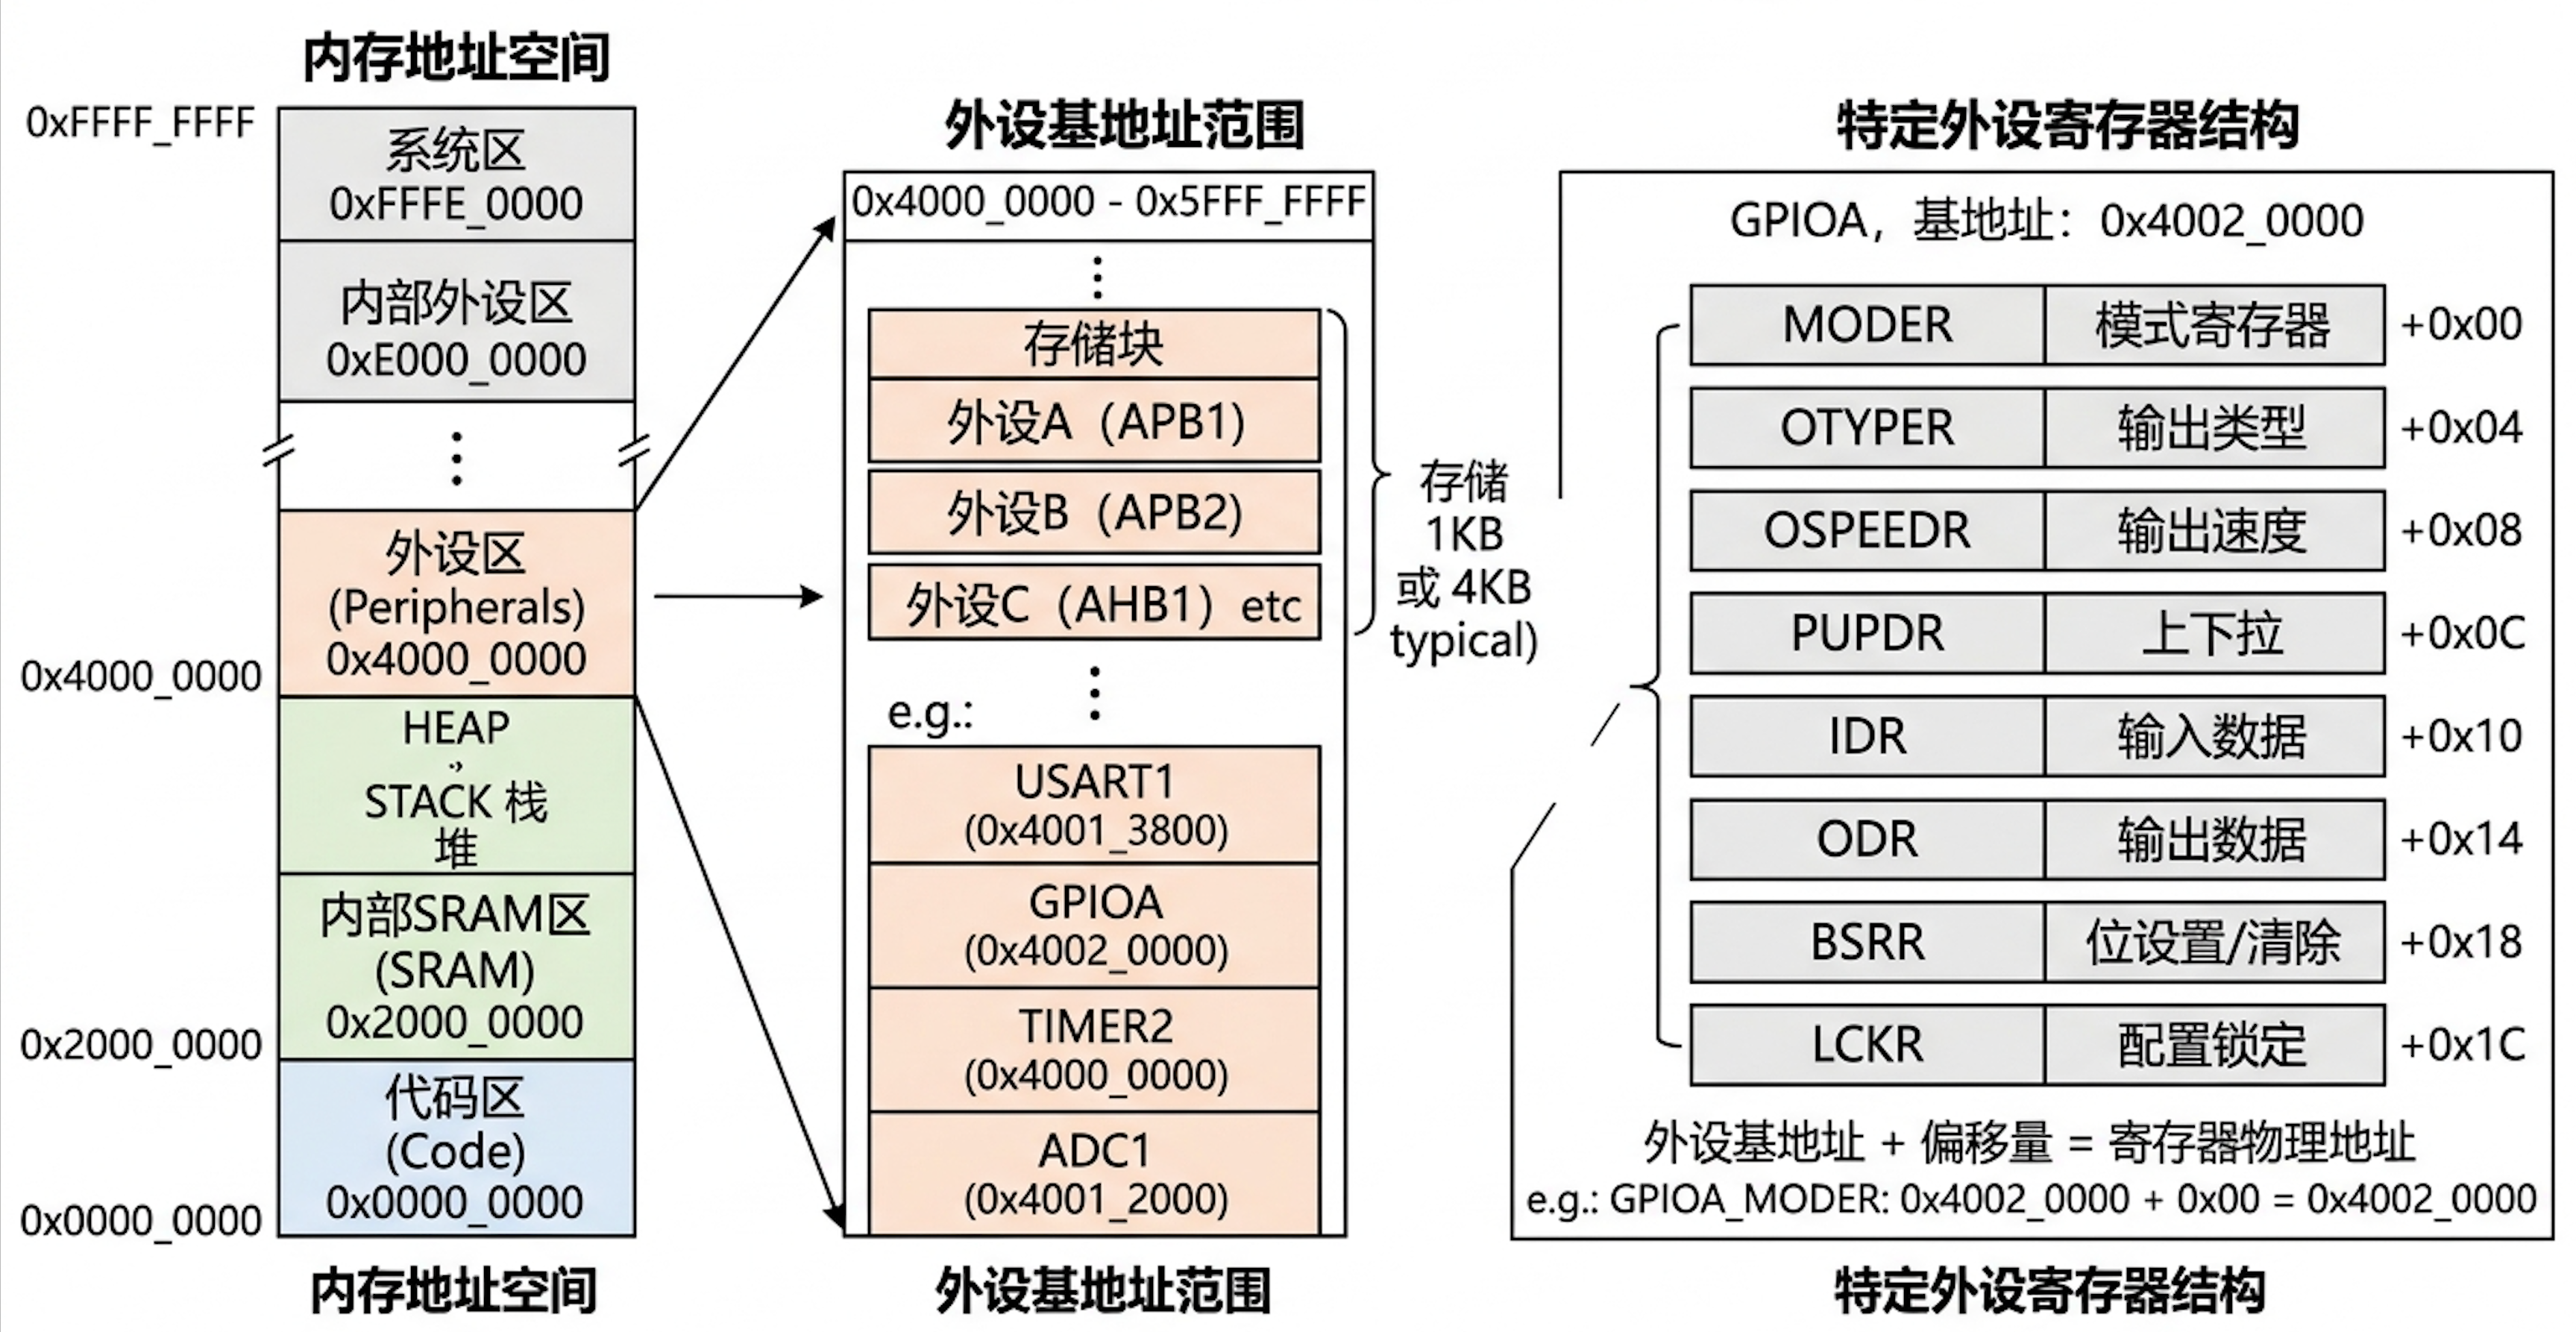
\includegraphics[width=0.85\textwidth]{figures/Arm架构图.png}
\caption{ARM Cortex-M 内存地址空间布局}
\label{fig:memory-map}
\end{figure}

外设寄存器按照功能可分为控制寄存器、状态寄存器和数据寄存器三类。控制寄存器用于配置外设的工作模式和参数，如 USART 的 CR1 可设置波特率、数据位长度等。状态寄存器反映外设的当前工作状态，如 USART 的 SR 包含发送缓冲区空（TXE）、接收缓冲区非空（RXNE）等标志位，其值由硬件自动更新。数据寄存器用于数据传输，如 USART 的 DR 用于发送和接收数据，访问数据寄存器通常会触发外设执行相应操作。

除 MMIO 外，中断（Interrupt）和直接内存访问（Direct Memory Access, DMA）也是嵌入式固件常见的外设操作方式。中断机制通过 NVIC 将外设事件（如串口接收完成、定时器溢出）异步通知给处理器，处理器在中断服务函数中完成状态更新或任务唤醒。DMA 机制允许外设在不经过 CPU 逐字搬运的情况下，直接与内存进行批量数据传输，常用于串口、SPI、ADC 等场景，以降低 CPU 开销并提升吞吐。

在固件仿真与驱动替换场景下，这三种机制往往共同出现：MMIO 负责寄存器读写与状态轮询，中断负责事件驱动控制流切换，DMA 负责高频数据搬运路径。若仅建模 MMIO 而忽略中断和 DMA，可能导致任务调度时序不一致、数据路径不完整或覆盖率评估偏差。因此，后续静态分析与动态验证需要同时关注寄存器访问模式、中断处理路径以及 DMA 相关配置与回调逻辑。

\section{物联网操作系统与驱动}
\label{sec:os}

\subsection{实时操作系统概述}
\label{sec:rtos}

实时操作系统（Real-Time Operating System, RTOS）是物联网设备中广泛采用的管理任务调度和资源分配的软件系统。RTOS 能够及时响应外部事件或数据，并在规定的时间内完成任务，其工作原理是通过一个实时任务调度器来管理系统资源，按照优先级或者时间片来分配 CPU 时间给不同的任务，保证重要或者紧急的任务优先执行。

物联网领域常见的 RTOS 包括 FreeRTOS\cite{freertos}、Zephyr\cite{zephyr}、RT-Thread\cite{rtthread} 等。FreeRTOS 是 Amazon 开源的实时操作系统，专为微控制器和小型微处理器设计，内核精简，最小可运行在不到 10KB 的 RAM 上，是物联网领域使用最广泛的 RTOS 之一。Zephyr 是 Linux 基金会管理的开源实时操作系统，支持多种处理器架构，提供更完整的操作系统功能，包括文件系统、网络协议栈、设备驱动模型等，采用模块化设计以平衡功能丰富性和资源占用。RT-Thread 是中国开源社区主导开发的实时操作系统，采用微内核架构，并提供了丰富的组件生态。

\begin{figure}[htbp]
\centering
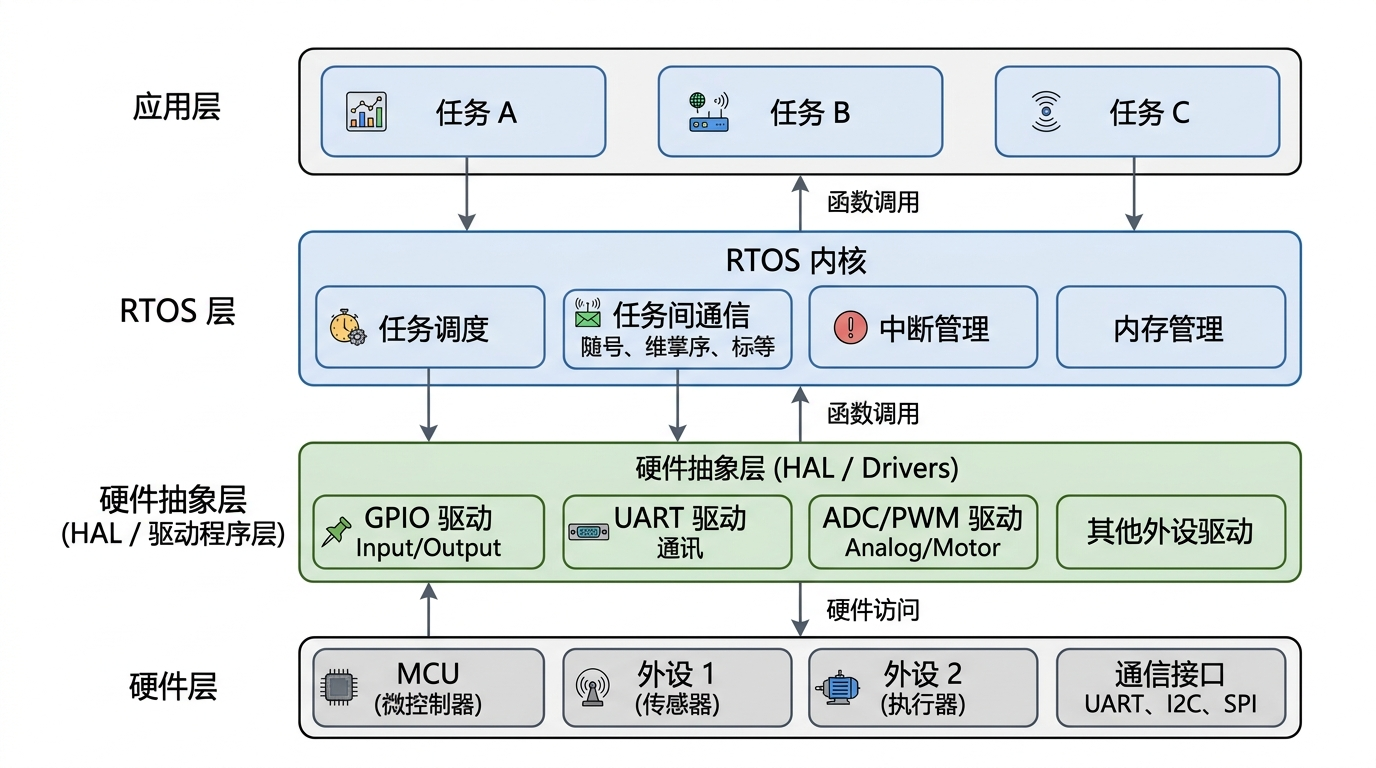
\includegraphics[width=0.85\textwidth]{figures/搭载RTOS的嵌入式固件的系统架构图.png}
\caption{搭载 RTOS 的嵌入式固件系统架构图}
\label{fig:rtos-arch}
\end{figure}

搭载 RTOS 的嵌入式固件通常采用分层架构，如图~\ref{fig:rtos-arch}所示。整个系统自底向上依次为硬件层、硬件抽象层（HAL）、操作系统内核以及应用层。硬件层包含 MCU 及各类外设；HAL 层封装了对底层寄存器的访问细节；RTOS 内核负责任务调度、中断管理和资源分配；应用层则实现具体的业务逻辑。固件运行过程中，应用程序通过 RTOS 提供的系统调用和驱动接口访问硬件资源，而非直接操作寄存器。这种分层结构使得驱动函数替换成为可能：仿真器可以在 HAL 层或驱动框架层拦截函数调用，用宿主机侧实现替代原始的硬件操作，从而在不修改上层应用逻辑的前提下实现固件的仿真执行。

\subsection{硬件抽象层}
\label{sec:hal}

硬件抽象层（Hardware Abstraction Layer, HAL）是嵌入式软件架构中的关键组成部分，它位于硬件驱动层和上层应用之间，为应用程序提供统一的硬件访问接口。HAL 层的核心目标是屏蔽底层硬件的差异性，使得上层应用代码可以在不同的硬件平台之间移植，而无需修改业务逻辑。

HAL 层的接口设计遵循统一的命名和功能规范。以 STM32 HAL 库为例，每个外设类型提供初始化函数（如 \texttt{HAL\_UART\_Init}）、数据传输函数（如 \texttt{HAL\_UART\_Transmit}）、状态查询函数（如 \texttt{HAL\_UART\_GetState}）和中断管理函数（如 \texttt{HAL\_UART\_Receive\_IT}）。由于 HAL 函数封装了底层硬件操作细节，仿真器可通过替换 HAL 层函数来实现硬件行为模拟，无需深入理解寄存器语义，相比寄存器级模拟更加高效且易于实现。

\section{开源程序静态分析技术}
\label{sec:program-analysis}

前两节介绍了物联网设备的硬件架构和驱动软件分层模型，明确了固件中驱动函数与硬件交互的基本方式。要实现驱动函数的自动化分析和替换，首先需要一种能够精确识别代码中 MMIO 访问模式和函数间数据流关系的分析手段。在静态分析引擎的选型上，本文考量了基于 LLVM/Clang 和基于 CodeQL 两种方案：基于 LLVM/Clang 的方案需要将嵌入式固件的构建工具链从 ARM GCC 切换到 Clang，而 CMSIS 头文件、厂商设备描述头文件以及 \texttt{\_\_attribute\_\_}、\texttt{\_\_IO} 等 ARM GCC 扩展语法在 Clang 下的兼容性尚不完整，迁移成本较高；CodeQL 通过在构建过程中拦截编译器调用来捕获源码信息，无需替代原始编译器，可直接在 ARM GCC 工具链上工作，无需修改固件工程的编译配置。基于上述分析，本研究选择 CodeQL 作为静态分析引擎，本节介绍其核心原理。

\subsection{CodeQL 代码分析平台}

CodeQL 是 GitHub 开发的语义级代码分析平台，支持多种编程语言（包括 C/C++、Java、Python、JavaScript 等）的安全漏洞检测和代码质量分析。CodeQL 的核心思想是将源代码转换为可查询的数据库，然后通过声明式查询语言（QL）进行灵活的分析。与传统基于规则的静态分析工具不同，CodeQL 提供了表达力丰富的查询语言，研究人员可以通过编写查询来查找特定的代码模式、追踪数据流、分析控制依赖等复杂问题。

CodeQL 的工作原理分为两个阶段。第一阶段是数据库构建，CodeQL 对源代码进行解析，生成抽象语法树（AST）、控制流图（CFG）、数据流图（DFG）等多层次的结构化表示，并将这些信息存储在数据库中。第二阶段是查询执行，研究人员使用 QL 语言编写查询，在数据库上执行，获取分析结果。CodeQL 的查询语言基于 Datalog，采用谓词逻辑的表达方式，能够自然地表达“所有存在某种模式的代码片段”或“从源点到汇点的数据流路径”等复杂查询。

CodeQL 在程序分析领域应用广泛，包括安全漏洞检测（如 SQL 注入、缓冲区溢出）、代码质量分析（如死代码检测、复杂度分析）、以及依赖关系分析（如函数调用图、数据流追踪）。本研究利用 CodeQL 的数据流追踪能力，建立 MMIO 访问与函数参数之间的关联关系，为驱动函数识别和语义分析提供支撑。

\section{物联网设备固件仿真与模糊测试}
\label{sec:fuzz}

静态分析能够识别驱动函数及其硬件访问模式，但要验证替换后固件的正确性，还需要将固件在仿真环境中动态执行并进行测试。固件仿真是物联网安全研究的重要技术手段。由于物联网设备的硬件多样性和封闭性，直接在真实设备上进行安全测试面临诸多困难。固件仿真技术通过软件模拟硬件环境，使研究人员能够在通用计算平台上运行和分析嵌入式固件，从而降低测试成本并提高效率。模糊测试作为一种高效的漏洞挖掘技术，与固件仿真相结合，能够在仿真环境中自动化地发现固件中的安全漏洞。

\subsection{QEMU 仿真器}

QEMU\cite{qemu} 是目前应用最广泛的开源机器仿真器，支持多种处理器架构和外设仿真，其设计目标是提供高性能、高可移植性的系统仿真能力，使其成为固件仿真研究的重要基础平台。QEMU 支持两种主要的仿真模式：用户模式仿真（User Mode Emulation）允许在一种架构上运行为另一种架构编译的单个程序，适用于分析用户空间程序；系统模式仿真（System Mode Emulation）提供完整的硬件系统仿真，包括处理器、内存、中断控制器、外设等组件，可以运行完整的操作系统或裸机固件，这是固件仿真的主要工作模式。

QEMU 的核心是动态二进制翻译引擎（Tiny Code Generator, TCG），它将目标架构的指令块翻译为中间表示（IR），然后再将 IR 翻译为宿主机指令，这种两级翻译机制使 QEMU 能够支持多种目标架构和宿主架构的组合。为了提高性能，TCG 采用即时编译（JIT）技术，将翻译结果缓存在内存中供后续执行重复使用。

Unicorn\cite{unicorn} 是基于 QEMU 的 TCG 引擎开发的轻量级 CPU 模拟器，专门针对安全研究和逆向工程场景优化。与 QEMU 提供完整系统级仿真的设计不同，Unicorn 去除了 QEMU 的系统级组件和外设仿真，只保留指令集模拟核心，因此具有更好的灵活性和可控性。Unicorn 提供了丰富的钩子（Hook）机制，允许用户在指令执行、内存访问、中断触发等事件上注册自定义回调函数，从而在不修改模拟器源码的情况下实现对执行过程的细粒度监控和干预。此外，Unicorn 以库的形式提供编程接口（支持 Python、C 等多种语言），便于嵌入到其他工具链中。本研究选用 Unicorn 作为固件动态测试的仿真引擎，利用其 ARM Thumb 模式模拟 ARM Cortex-M 系列微控制器，并通过钩子机制实现驱动函数拦截、运行日志采集和仿真数据注入等功能。



\subsection{模糊测试技术}

模糊测试（Fuzzing）是一种自动化软件测试技术，通过向目标程序输入大量随机、半随机或结构化的测试用例，来发现程序中的安全漏洞和缺陷\cite{manesArtScienceEngineering2021}。模糊测试的基本工作流程包括：生成或变异测试用例、将测试用例输入目标程序、监控程序执行状态（如崩溃、断言失败、内存错误等）、记录和分析异常。

American Fuzzy Lop（AFL）\cite{aflplusplus_paper} 是最具影响力的覆盖率引导模糊测试工具之一。AFL 的核心思想是通过代码插桩技术记录程序执行过程中的覆盖率信息，利用这些信息指导测试用例的变异和选择，优先保留能够触发新执行路径的测试用例，从而在有限的测试时间内探索更多的程序状态，提高漏洞发现的概率。AFL 的工作流程包含两个核心环节：覆盖率记录和变异策略。在覆盖率记录环节，AFL 通过编译时插桩或运行时插桩（利用 QEMU 的动态翻译功能）在目标程序中插入覆盖率记录代码，记录程序执行过程中经过的基本块和边。在变异策略环节，AFL 维护一个测试用例队列，不断从队列中选择测试用例，对其进行变异，执行变异后的测试用例，并根据覆盖率变化决定是否将新用例加入队列。AFL 的变异策略包括位翻转、字节删除、字节插入、块拼接、算术运算等多种操作，能够产生多样化的测试输入。通过这种迭代式的测试和筛选机制，AFL 能够逐步探索程序的各种执行路径，自动发现潜在的漏洞和缺陷。

在嵌入式固件模糊测试领域，AFL 常与仿真器（如 QEMU）结合使用。研究者在 QEMU 的动态翻译机制基础上实现插桩，使 AFL 能够对在仿真环境中运行的固件进行模糊测试。这种方法不需要修改固件源码，能够直接对二进制固件进行测试，并提升测试流程的自动化程度和可扩展性。

\section{大模型代码分析智能体框架}
\label{sec:llm}

前四节分别介绍了固件仿真的硬件基础、驱动软件模型、静态分析技术和动态测试方法，构成了完整的固件仿真技术链。然而，现有方法在驱动函数定位、语义理解和替换代码生成等关键环节仍高度依赖人工，自动化程度不足。近年来，大语言模型在代码理解和生成方面展现出强大的能力，为自动化程序分析提供了新的技术途径。本节重点阐述代码分析工作流范式和基于 LLM 的智能体开发框架，为后续章节的驱动函数分析和替换工作奠定技术背景。

\subsection{代码分析工作流设计模式}
\label{sec:workflow_paradigm}

基于 LLM 智能体框架构建代码分析系统时，研究者提出了多种工作流设计模式。这些模式为处理代码分析任务中常见的逻辑推理、工具调用、多步骤协作等挑战提供了系统化思路。

\textbf{ReAct 模式}：ReAct（Reasoning + Acting）将推理与行动交替进行\cite{Yao_2022}。在代码分析中，LLM 可先推理分析目标（如“需要理解该函数的调用关系”），再调用静态分析工具获取信息，观察结果后继续下一步推理。该模式使 LLM 能够动态收集信息并逐步完成复杂分析。

\textbf{规划-执行模式}：该模式将任务分为规划与执行两阶段\cite{wang2023plan}。规划阶段由 LLM 将复杂任务分解为步骤化的执行计划，明确每步的输入、输出和依赖关系；执行阶段按序完成各步骤，并可根据中间结果动态调整后续计划。其优势在于结构清晰、便于调试和过程监控。在代码分析场景中，该模式适用于流程较为固定的任务，例如驱动函数替换可分解为“拉取上下文→语义分类→策略选择→代码生成→质量校验”等确定步骤，每步的输出作为下一步的输入，相比 ReAct 的自由探索更易于控制执行流程和定位错误环节。

\textbf{多智能体协作模式}：该模式使用多个专门化的智能体协同完成任务\cite{dong2024selfcollaboration}。例如在驱动函数替换中，可设计分析智能体、生成智能体、验证智能体与协调智能体，通过消息传递或共享状态完成复杂代码分析与生成任务。本研究在驱动函数替换模块中，综合运用了 ReAct 模式与多智能体协作模式，以应对硬件相关代码替换的复杂性与正确性要求。

上述工作流设计模式为 LLM 驱动的代码分析系统提供了理论指导，而将其落地实现则需要依赖成熟的智能体开发框架。下节介绍本研究选用的 LangChain/LangGraph 框架及其核心机制。

\subsection{LLM 智能体开发框架}
\label{sec:llm_framework}

为了更好地利用大语言模型构建复杂的应用系统，研究人员开发了多种智能体框架。这些框架提供了结构化的方式来组织 LLM 的调用、管理状态、集成外部工具，使开发者能够构建可靠、可扩展的 LLM 应用。

\subsubsection{LangChain 框架}

LangChain 是目前最流行的 LLM 应用开发框架之一，提供了模型、提示模板、链、代理、工具和记忆等核心组件。模型组件封装了与不同 LLM 提供商的交互接口，便于切换和比较。提示模板允许开发者定义带变量的提示词，在运行时动态填充，提高复用性。链将多个组件按顺序组合，构建复杂的处理流程。代理是更高级的抽象，允许 LLM 根据用户输入自主选择合适的工具（如搜索引擎、代码执行器）并决定后续行动。工具是代理可以调用的外部功能，框架提供了大量内置工具，开发者也可自定义。记忆组件维持应用在多次调用之间的状态，例如在多轮对话中存储历史对话。

\subsubsection{LangGraph 状态图}

LangGraph 是 LangChain 生态中用于构建有状态、可循环的智能体工作流的库。与LangChain的链式结构不同，LangGraph 基于状态图的概念，状态在各个节点之间传递和更新。节点是处理单元，边定义转换关系并支持条件分支和循环，适用于迭代优化等场景。LangGraph 还支持检查点机制，可将工作流状态持久化存储，支持长时间运行任务的暂停和恢复。

\section{本章小结}
\label{sec:bg_summary}

本章按照“了解分析目标→掌握分析方法→引入自动化手段”的逻辑，依次介绍了物联网设备固件仿真研究所需的技术基础。首先阐述了 ARM Cortex-M 架构特性以及 MMIO、中断、DMA 三类外设操作方式，明确了固件与硬件交互的底层方式；然后介绍了实时操作系统与硬件抽象层的概念，分析了搭载 RTOS 的嵌入式固件的分层架构及其对驱动函数替换的支撑作用；接着介绍了以 CodeQL 为代表的开源程序静态分析技术的原理与选型依据，以及基于 QEMU/Unicorn 的固件仿真技术和 AFL 模糊测试方法；最后讲解了大语言模型代码分析的智能体框架设计模式（ReAct、规划-执行、多智能体协作）以及 LangGraph 开发框架的核心机制，为利用 LLM 实现驱动函数自动化分析与替换提供了技术支撑。
  % 背景知识与相关技术
\chapter{系统设计}
\label{chap:design}

\usetikzlibrary{arrows.meta,positioning,calc}

\begin{figure}[htbp]
\centering
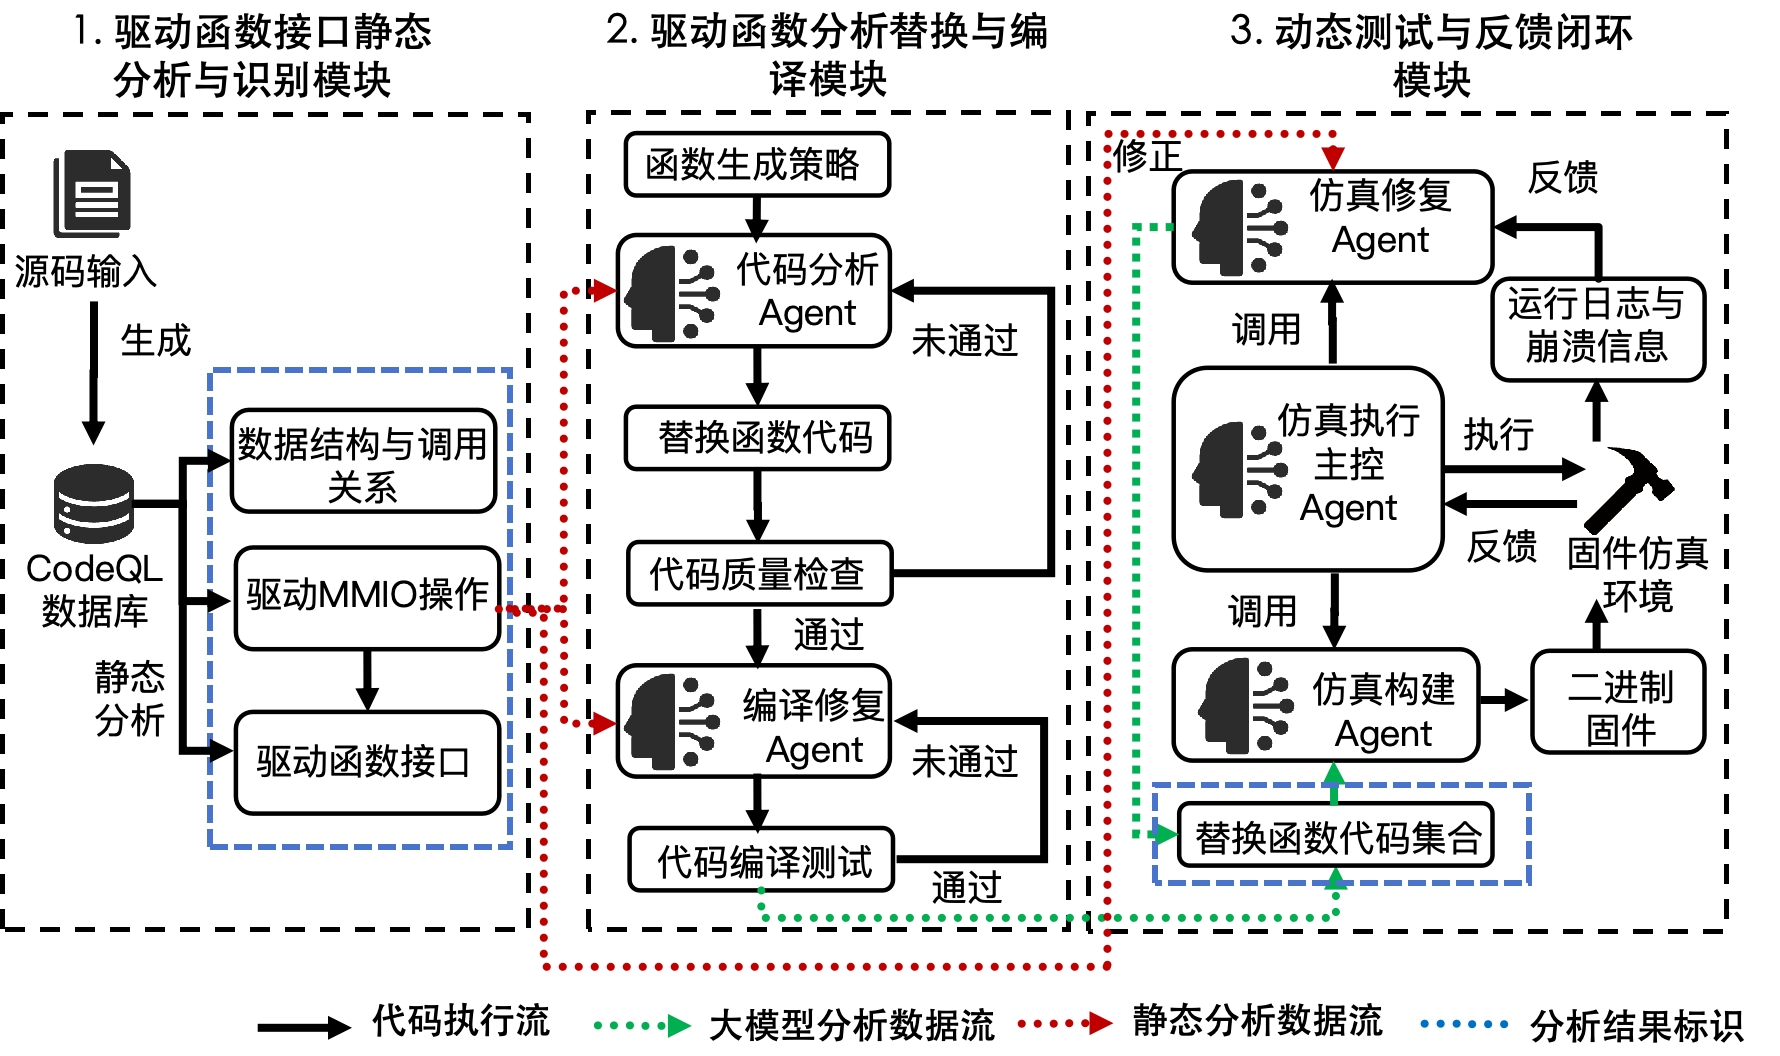
\includegraphics[width=0.95\textwidth]{figures/system_architecture.png}
\caption{系统整体架构图}
\label{fig:arch}
\end{figure}

本研究设计并实现了基于驱动程序替换的固件仿真系统，该系统分为三个模块：（1）驱动函数接口静态分析与识别模块；（2）驱动函数分析、替换与编译模块；（3）动态测试反馈闭环模块。整体方案架构图如图~\ref{fig:arch}所示。

驱动函数接口静态分析与识别模块首先接受固件源码，然后通过 CodeQL 静态分析引擎建立抽象语法树构建的数据库，通过预定义的查询规则从固件源码中提取驱动相关信息，包括驱动函数接口、驱动 MMIO 操作、依赖数据结构与函数间调用关系等信息，并以统一的数据模型对外提供查询接口。

驱动函数分析、替换与编译模块首先接受驱动函数接口静态分析与识别模块输出的驱动函数信息，然后针对各驱动函数进行类型分类并通过合适的函数替换策略生成可替代实现，之后对生成的替换函数代码做质量检查，如果质量检查通过，则将替代实现集成回工程并驱动构建，进一步通过交叉编译验证替换代码是否存在编译错误。如果存在编译错误，则触发编译修复智能体进行修复，修复完成后再次通过交叉编译验证。该模块采用 LangGraph 智能体框架实现复杂的推理和决策流程，确保生成的替换代码既满足语义保持性要求，又能够正常通过交叉编译工具链的验证。

动态测试反馈闭环模块首先接受驱动函数分析、替换与编译模块输出的替换代码，然后在仿真环境中运行固件，采集运行日志、崩溃信息等，并将错误信息结构化，触发闭环修复智能体对嵌入式程序进行重新分析与替换代码修正，修正完成后再次通过闭环构建智能体交叉编译生成可执行的二进制固件程序，再次在仿真环境中运行固件，如此循环，直至替换代码通过仿真测试。通过多智能体协作，该模块构建"生成-测试-反馈-修正"的闭环机制，使固件构建仿真与自修复的全过程实现自动化。

为精确定义系统的输入输出关系，以下给出端到端映射的形式化描述。设固件源码工程为 $P$，固件中的函数集合为 $F$，MMIO 结构体实例集合为 $M$，驱动函数类别集合为 $C$，替换策略集合为 $S$。系统的端到端功能可形式化为以下映射：
\begin{align}
\textit{StaticAnalysis}: P &\to (D, R, G) \label{eq:static} \\
\textit{Classify}: D &\to C \label{eq:classify} \\
\textit{Replace}: D \times C &\to D' \label{eq:replace} \\
\textit{Verify}: D' &\to \{\textit{pass}, \textit{fail}\} \label{eq:verify} \\
\textit{Emulate}: P' &\to (O, E) \label{eq:emulate}
\end{align}
其中，式~\ref{eq:static}~中 $D \subseteq F$ 为识别出的驱动函数集合，$R$ 为 MMIO 访问点集合，$G = (F, E_c)$ 为函数调用图（$E_c$ 为调用边集合）；式~\ref{eq:classify}~将每个驱动函数映射到其语义类别；式~\ref{eq:replace}~对每个驱动函数 $f \in D$ 生成替换实现 $f' \in D'$；式~\ref{eq:verify}~对替换实现进行多层验证；式~\ref{eq:emulate}~中 $P'$ 为替换后的工程，$O$ 为仿真运行输出，$E$ 为运行时错误集合。系统通过迭代执行"替换$\to$验证$\to$仿真$\to$反馈"闭环，直至 $E = \emptyset$ 或达到最大迭代次数。

\section{驱动函数接口静态分析与识别模块设计}

本模块是整个方案的基础支撑层，负责自动、精准地定位固件中与硬件交互的代码，并将其抽象为标准化的"可查询知识库"。模块的核心职责是建立从源码到硬件依赖信息的映射，识别固件中与硬件交互的函数，确定函数访问硬件的方式（如直接寄存器访问、HAL 库调用或间接句柄操作），并分析函数之间的调用依赖关系。

在静态分析引擎的选型上，本模块需要对比源码级方案内部的两种技术路线：基于 LLVM/Clang 的分析和基于 CodeQL 的分析。

基于 LLVM/Clang 的分析方案（如 P2IM~\cite{fengp2020p2im} 采用基于 LLVM IR 的启发式规则识别外设寄存器访问）在实际应用中面临工程兼容性问题。嵌入式固件的构建工具链通常与 ARM GCC 深度绑定：Zephyr RTOS 通过 west 构建系统默认调用 \texttt{arm-none-eabi-gcc} 进行交叉编译，STM32CubeIDE、MCUXpresso 等厂商 IDE 同样基于 ARM GCC 工具链；嵌入式工程中广泛使用的 CMSIS 头文件、芯片厂商提供的设备描述头文件以及 \texttt{\_\_attribute\_\_}、\texttt{\_\_IO}、\texttt{\_\_ASM} 等 ARM GCC 扩展语法，Clang 的兼容性尚不完整。若采用基于 Clang 的源码分析工具，需要将整个构建工具链从 ARM GCC 切换到 Clang，这一过程涉及重新配置构建系统、适配厂商头文件中的编译器扩展语法以及处理链接器脚本差异等问题，迁移成本较高。此外，部分嵌入式工程的构建脚本使用 ARM GCC 特有的编译选项（如 \texttt{-mcpu=cortex-m4}、\texttt{-mfpu=fpv4-sp-d16} 等），Clang 对这些选项的语义解释存在差异，可能导致分析结果与实际编译行为不一致。

CodeQL 采用与编译器无关的数据库构建方式：通过在构建过程中拦截编译器调用来捕获源码信息，而非替代原始编译器执行编译。因此，CodeQL 可以直接在 ARM GCC 工具链的构建流程上工作，无需修改固件工程的编译配置。CodeQL 将源码构建为包含 AST、控制流图和数据流图的综合数据库，支持声明式查询语言和全局污点追踪，能够在不运行固件的情况下跨文件追踪 MMIO 基址常量的传播路径，为后续的智能替换提供基础数据。与运行时方法相比（如 HALucinator~\cite{clements2020halucinator} 通过 QEMU 的内存追踪识别外设访问），CodeQL 无需先实现完整的外设模型即可工作。

模块采用静态分析技术构建包含语法树、控制流图和数据流图的综合数据库，通过设计的查询规则识别 MMIO 结构体实例和字段访问，进而识别涉及硬件访问的驱动函数，为替换模块提供精确的语句定位信息。模块输出的分析结果包含驱动函数列表、MMIO 访问操作、函数调用关系图和数据结构信息，这些结构化的分析结果被存储在统一的数据模型中，为下游模块提供可查询的知识库。

\subsection{MMIO 访问模式识别方法}

MMIO（Memory-Mapped I/O，内存映射 I/O）是一种将硬件外设的寄存器映射到处理器内存地址空间的机制。通过 MMIO，软件可以通过访问内存地址的方式与硬件外设进行交互，而不需要特殊的 I/O 指令。嵌入式厂商通常使用 C 语言结构体来定义 MMIO 寄存器映射，结构体的每个字段对应一个硬件寄存器，字段的偏移量与硬件规范中的寄存器地址偏移保持一致。

MMIO 结构体的典型代码示例如代码~\ref{lst:mmio-struct}所示。

\begin{lstlisting}[style=CStyle,language=C,caption=MMIO 结构体示例,label=lst:mmio-struct]
// STM32 UART寄存器映射示例
typedef struct {
    __IO uint32_t CR1;    // 控制寄存器1
    __IO uint32_t CR2;    // 控制寄存器2
    __IO uint32_t CR3;    // 控制寄存器3
    __IO uint32_t BRR;    // 波特率寄存器
    __IO uint32_t GTPR;   // 保护时间与预分频寄存器
    __IO uint32_t RTOR;   // 接收超时寄存器
    __IO uint32_t RQR;    // 请求寄存器
    __IO uint32_t ISR;    // 中断与状态寄存器
    __IO uint32_t ICR;    // 中断标志清除寄存器
    __IO uint32_t RDR;    // 接收数据寄存器
    __IO uint32_t TDR;    // 发送数据寄存器
} USART_TypeDef;

// 通过强制类型转换创建MMIO实例
#define USART1_BASE    (0x40011000UL)
USART_TypeDef *USART1 = (USART_TypeDef *)USART1_BASE;
\end{lstlisting}

定位 MMIO 结构体实例是识别硬件相关代码的关键步骤。本研究总结出三种典型的 MMIO 实例定位模式，分别如代码~\ref{lst:direct-cast}、代码~\ref{lst:indirect-init}和代码~\ref{lst:pointer-param}所示。

\textbf{模式一：直接地址强转}。这类代码将固定外设基地址强制转换为外设寄存器结构体指针，常见于寄存器定义的头文件中。在代码中呈现为类似 \texttt{\#define USART1 ((USART\_TypeDef *)USART1\_BASE)} 的宏定义，后续代码直接对该指针进行字段访问如 \texttt{USART1->DR}、\texttt{USART1->CR1}。

\begin{lstlisting}[style=CStyle,language=C,caption=直接地址强转模式示例,label=lst:direct-cast]
// 驱动源码示例：直接地址强转模式
#define USART1_BASE 0x40011000UL
#define USART1 ((USART_TypeDef *)USART1_BASE)
#define USART2 ((USART_TypeDef *)USART2_BASE)
#define USART3 ((USART_TypeDef *)USART3_BASE)

void uart_init_direct(void) {
    USART1->CR1 = 0x2000;  // 直接对强转实例进行寄存器访问
    USART1->BRR = 0x0341;
}
\end{lstlisting}

\textbf{模式二：间接初始化}。这类代码通过句柄（handle）、配置表（descriptor/config table）等间接结构，将外设基地址赋值给某个"寄存器块指针成员"，后续通过该成员完成寄存器访问。在 STM32 HAL 生态中，这类成员常命名为 \texttt{Instance}。在代码中呈现为初始化时的赋值语句如 \texttt{huart->Instance = COM\_USART[COM]}，后续寄存器访问呈现为多级解引用如 \texttt{huart->Instance->DR}。在基于配置表的驱动中，也可能呈现为 \texttt{handle.Instance = spi\_config[i].Instance} 这种从配置表复制的形式。

\begin{lstlisting}[style=CStyle,language=C,caption=间接初始化模式示例（HAL句柄和配置表）,label=lst:indirect-init]
// 驱动源码示例：间接初始化模式（HAL句柄）
UART_HandleTypeDef huart;

void BSP_COM_Init(COM_TypeDef COM) {
    huart.Instance = COM_USART[COM];  // 将外设基地址赋值给Instance成员
    HAL_UART_Init(&huart);
    // 后续访问呈现为多级解引用
    huart.Instance->DR = data;
}

// 驱动源码示例：间接初始化模式（配置表）
typedef struct {
    USART_TypeDef *Instance;
    uint32_t BaudRate;
} SPI_Config;

SPI_Config spi_config[] = {
    {SPI1, 115200},
    {SPI2, 9600}
};

void rt_hw_spi_bus_init(void) {
    for (int i = 0; i < sizeof(spi_config)/sizeof(spi_config[0]); i++) {
        spi_bus_obj[i].handle.Instance = spi_config[i].Instance;
        // 通过配置表中的Instance赋值
    }
}
\end{lstlisting}

\textbf{模式三：常量指针参数}。这类代码通过函数参数接收 MMIO 结构体指针（寄存器块基址），常见于底层驱动或通用外设操作函数。在代码中呈现为函数定义的形参类型是某个寄存器结构体指针，函数体内部通过该参数访问寄存器字段，如 \texttt{void mmio\_uart\_init(USART\_TypeDef *uart) \{ uart->CR1 = 0x2000; \}}。调用者可以将模式一或模式二中的 MMIO 实例作为实参传入，如直接调用 \texttt{mmio\_uart\_init(USART1)} 或传入句柄成员 \texttt{mmio\_uart\_init(huart.Instance)}。

\begin{lstlisting}[style=CStyle,language=C,caption=常量指针参数模式示例,label=lst:pointer-param]
// 驱动源码示例：常量指针参数模式
void mmio_uart_init_pointer(USART_TypeDef *uart) {
    // 通过指针访问MMIO寄存器
    uart->CR1 = 0x2000;
    uart->BRR = 0x0341;
}

// 调用示例
void main(void) {
    // 直接传模式一的强转实例
    mmio_uart_init_pointer(USART1);

    // 传模式二的句柄成员
    mmio_uart_init_pointer(huart.Instance);

    return 0;
}
\end{lstlisting}

三种定位模式的对比如表~\ref{tab:mmio-patterns}所示。

设 $T$ 为 MMIO 寄存器结构体类型集合，$A$ 为外设基址常量集合，$H$ 为句柄结构体类型集合，$F$ 为函数集合，则三种定位模式可形式化定义为：

\textbf{模式一（直接地址强转）}：存在常量 $a \in A$ 和类型 $t \in T$，使得 $a$ 被显式转换为 $t^*$ 类型，即存在表达式 $\texttt{cast}(a) \to t^*$。后续通过该指针的字段访问构成 MMIO 操作：
$$\textit{DirectCast} = \{(a, t) \mid a \in A, t \in T, \exists\, \texttt{cast}(a): a \to t^*\}$$

\textbf{模式二（间接初始化）}：存在句柄 $h$（类型为 $\tau \in H$），其成员 $h.\textit{inst}$ 被赋值为 MMIO 实例的指针，后续通过 $h.\textit{inst} \to \textit{field}$ 进行字段访问：
$$\textit{IndirectInit} = \{(h, t) \mid h.\textit{inst} = \textit{ptr}, \textit{ptr} \to t^*, t \in T\}$$

\textbf{模式三（常量指针参数）}：存在函数 $f \in F$，其参数列表中包含类型为 $t^*$（$t \in T$）的形式参数，调用点传入 MMIO 实例指针作为实参：
$$\textit{PtrParam} = \{(f, t, i) \mid f.\textit{param}_i: t^*, t \in T\}$$

三种模式共同构成 MMIO 实例的完整识别规则集合 $\textit{MMIOInst} = \textit{DirectCast} \cup \textit{IndirectInit} \cup \textit{PtrParam}$。与已有方法不同，P2IM~\cite{fengp2020p2im} 通过运行时 fuzzing 探测外设行为，HALucinator~\cite{clements2020halucinator} 通过 QEMU 内存追踪识别外设访问，本研究从源码层面对 MMIO 访问模式进行了系统性的分类和形式化描述，为驱动函数的精确识别提供了可复用的查询规则。

\begin{table}[htbp]
\centering
\caption{MMIO 结构体实例定位模式对比}
\label{tab:mmio-patterns}
\footnotesize
\begin{tabular}{lp{5cm}l}
\toprule
\textbf{模式} & \textbf{描述} & \textbf{代码呈现} \\
\midrule
直接地址强转 & 将固定地址强制转换为外设结构体指针 & 整数常量$\to$结构体指针类型转换 \\
间接初始化 & 通过配置表将外设基地址赋值给句柄 & 结构体成员赋值为外设宏 \\
常量指针参数 & 函数以常量指针形式接收外设基址 & 参数类型为 MMIO 结构体指针 \\
\bottomrule
\end{tabular}
\end{table}

\subsubsection{查询规则设计原则}

为在 CodeQL 数据库中可靠地识别上述三种 MMIO 定位模式，本研究设计了相应的查询规则体系。查询规则的设计遵循以下原则：

\textbf{（1）结构体特征识别}。首先识别 MMIO 寄存器结构体，判定依据包括：结构体名称包含 \texttt{TypeDef}、\texttt{\_TypeDef}、\texttt{\_Registers} 等典型后缀；结构体字段类型以 \texttt{\_\_IO}（volatile 修饰）为主；字段偏移量与芯片参考手册中的寄存器地址偏移一致。查询规则通过匹配这些特征从数据库中提取候选 MMIO 结构体，过滤掉普通数据结构体。

\textbf{（2）基址常量识别}。MMIO 实例的基址通常以宏或枚举常量的形式定义，其数值范围为典型外设地址区间（如 STM32F4 的 APB1/APB2 总线地址 0x40000000--0x50000000）。查询规则通过识别数值落在已知外设地址区间内的常量表达式，过滤掉地址空间无关的普通整数常量，降低误报率。

\textbf{（3）类型转换链追踪}。对于模式一（直接地址强转），查询规则追踪从基址常量到结构体指针类型的显式转换表达式（C 语言中的 \texttt{(Type *)cast} 形式），并进一步追踪通过该指针的解引用和字段访问。对于模式二（间接初始化），查询规则通过数据流追踪识别从 MMIO 实例到句柄成员的赋值传播路径，再追踪句柄成员的字段访问。对于模式三（常量指针参数），查询规则匹配函数参数类型为 MMIO 结构体指针的函数定义，并追踪调用点传入的实际参数来源。

\textbf{（4）污点传播与边界控制}。为防止追踪范围过度扩散，查询规则设置传播边界条件：仅追踪通过指针解引用（\texttt{->} 操作符）和结构体字段访问的路径，不追踪算术运算后的指针偏移；传播深度限制在函数调用图的三层以内，避免跨模块追踪引入无关噪声。对于跨文件和跨编译单元的 MMIO 访问，通过 CodeQL 的全局数据流分析能力实现跨文件追踪。

上述查询规则的设计确保了 MMIO 识别的准确性和可扩展性：结构体特征识别和基址常量识别提供了高精度的起点，类型转换链追踪覆盖了三种定位模式的代码呈现形式，污点传播边界控制则在保证召回率的同时限制了误报范围。当需要支持新的 MCU 平台时，仅需更新基址常量的地址区间和结构体特征的后缀规则即可适配，无需修改核心查询逻辑。

\subsection{驱动函数定位准则}

静态分析模块的核心任务是识别固件中的驱动函数。本研究采用简单直接的定位准则：\textbf{凡是包含 MMIO 访问的函数，均定义为驱动函数}。这一定位准则的合理性在于：MMIO 访问是固件与硬件交互的最底层方式，包含寄存器读写的函数必然与硬件强相关，这类函数在仿真环境中无法直接执行，需要进行替换处理；而不包含 MMIO 访问的函数通常是纯软件逻辑，如数据处理、协议解析、状态管理等，在仿真环境中可以直接运行，无需替换。

设 $F$ 为固件中的函数集合，$M$ 为 MMIO 结构体实例集合，$A(f, m)$ 为谓词"函数 $f$ 访问 MMIO 实例 $m$ 的字段"，则驱动函数集合 $D$ 定义为：
$$D = \{f \in F \mid \exists m \in M: A(f, m)\}$$

驱动函数识别的流程如下：首先通过三种定位模式识别代码中的所有 MMIO 结构体实例；然后对每个 MMIO 结构体实例，追踪其字段访问表达式，记录访问的字段名、访问类型（读/写）、所在语句和所在函数；接着对所有包含 MMIO 字段访问的函数进行汇总，形成驱动函数列表；最后分析驱动函数之间的调用关系，构建函数调用图。

\subsection{数据流追踪方法}

系统以"MMIO 字段访问"为源点，以"函数参数、局部变量、返回值"为汇点，构建数据流配置并追踪路径。追踪目的包括：

1. 确定哪些函数参数最终影响了 MMIO 访问；
2. 识别需要保留的业务逻辑与需要替换的硬件操作；
3. 为替换模块提供精确的语句定位信息。

\subsubsection{追踪配置设计}

数据流追踪基于 CodeQL 提供的污点分析框架实现。系统配置了两类追踪路径：

\textbf{正向追踪}：从 MMIO 基址常量出发，沿赋值语句、函数参数传递、结构体字段赋值等路径追踪 MMIO 实例的传播，识别所有通过该实例进行字段访问的代码位置。正向追踪的源点为识别出的 MMIO 基址常量表达式，汇点为结构体字段访问表达式（即 \texttt{expr->field} 形式的访问）。

\textbf{反向追踪}：从 MMIO 字段访问表达式出发，反向追踪数据来源，确定访问的值是否来源于函数参数或外部输入。反向追踪用于区分"配置型访问"（值由软件写入寄存器，如初始化阶段设置波特率）和"状态型访问"（值从寄存器读出，如轮询等待标志位），前者通常可安全替换，后者需要通过仿真注入接口模拟硬件状态。

\subsubsection{追踪复杂度分析}

设固件中函数数量为 $n$，平均函数调用深度为 $d$，平均每个函数的 MMIO 访问点数量为 $k$。数据流追踪的时间复杂度取决于 CodeQL 污点分析引擎的实现，其理论复杂度为 $O(n \cdot d \cdot k)$：$n$ 为候选源点函数的数量，$d$ 为追踪的最大传播深度（受边界条件约束），$k$ 为每个函数中需要检查的汇点数量。在本研究的测试固件中，$n$ 的取值范围为 10--130，$d$ 通常不超过 5，$k$ 的平均值约为 3，因此单次追踪的计算开销在可接受范围内。空间复杂度为 $O(n \cdot d)$，主要用于存储追踪路径的中间结果。

需要指出的是，CodeQL 的污点分析基于静态近似，可能存在以下局限：一是无法处理通过函数指针或虚函数表进行的间接调用，这类间接调用在嵌入式固件中相对少见；二是对运行时才能确定的数组索引和条件分支采用保守估计，可能引入少量无关追踪路径。在实际应用中，上述局限对驱动函数识别的召回率影响有限，因为嵌入式驱动代码的函数调用关系通常较为明确，间接调用的使用场景较少。

\subsection{统一数据模型设计}

系统定义了统一的数据模型来表示分析结果，包括 \texttt{FunctionInfo}（函数基本信息）、\texttt{MMIOAccess}（MMIO 访问点）等结构，为上层模块提供标准化查询接口。数据模型采用 Python 数据类（dataclass）定义，支持序列化和反序列化。

数据模型包括函数信息模型（包含函数名、文件路径、行号、签名、返回类型、参数列表、分类、源码、调用关系等信息）、MMIO 访问点模型（包含结构体类型、字段名、访问类型、行号、所在函数、上下文代码等）和项目分析结果模型（包含项目路径、CodeQL 数据库路径、所有函数、MMIO 访问点、函数调用图、驱动函数列表、分析时间戳等）。这些数据模型通过 JSON 序列化存储在缓存层，供后续模块查询和使用。

\section{驱动函数分析、替换与编译模块设计}

驱动函数分析、替换与编译模块负责语义理解和代码生成，采用大语言模型驱动的智能体架构，实现从函数分类、代码生成、质量验证到编译集成的完整自动化流程。该模块采用"语义分析$\to$代码生成$\to$质量验证$\to$编译集成$\to$错误修复"的迭代优化模式，通过多轮迭代逐步提升替换质量，直至生成能够在仿真环境中正常运行的替换代码。

在智能体框架的选型上，本模块选择 LangGraph 作为编排框架。驱动函数替换涉及多轮推理决策（函数分类、策略选择、代码生成、质量验证），且各步骤之间存在复杂的条件依赖和迭代关系。LangGraph 基于图式状态机模型，天然支持条件分支和循环结构，能够精确表达"分类→生成→验证→修复"的迭代工作流；同时支持工具调用（Tool Calling）机制，可以将静态分析查询、编译构建等外部能力封装为图节点，实现智能体与工程环境的深度集成。相比纯对话式框架，LangGraph 对执行流程的控制粒度更细，能够精确控制每步的输入输出和状态传递，这对于需要严格保证函数签名一致性和编译正确性的驱动替换场景尤为必要。

\subsection{分析替换与编译智能体工作流设计}

工作流以\textbf{单个驱动函数}为粒度调度：每轮从静态分析模块或任务队列中取定一条驱动函数记录（含签名、源码片段、MMIO 访问上下文等），在图式状态机中顺序执行，直至该函数被判定为无需替换并结束，或替换实现通过校验与编译并被采纳。为便于叙述与实现解耦，整条流水线在逻辑上划分为\textbf{驱动函数分析与替换代码生成}、\textbf{替换代码修正与编译集成}两个子模块；前者由\textbf{分析智能体}主导完成上下文拉取、分类与候选替换生成，后者由\textbf{编译修复智能体}在工程侧完成定义校验、构建与失败修复。为避免混淆，下文将模块二中的编译修复智能体称为"编译修复智能体"，将模块三中负责运行时错误后重新构建的智能体称为"闭环构建智能体"，两者职责不同：前者处理替换代码首次集成时的编译错误（如语法错误、类型不匹配），后者处理动态反馈闭环中经仿真验证发现运行时错误后的重新构建。

\begin{figure}[htbp]
    \centering
    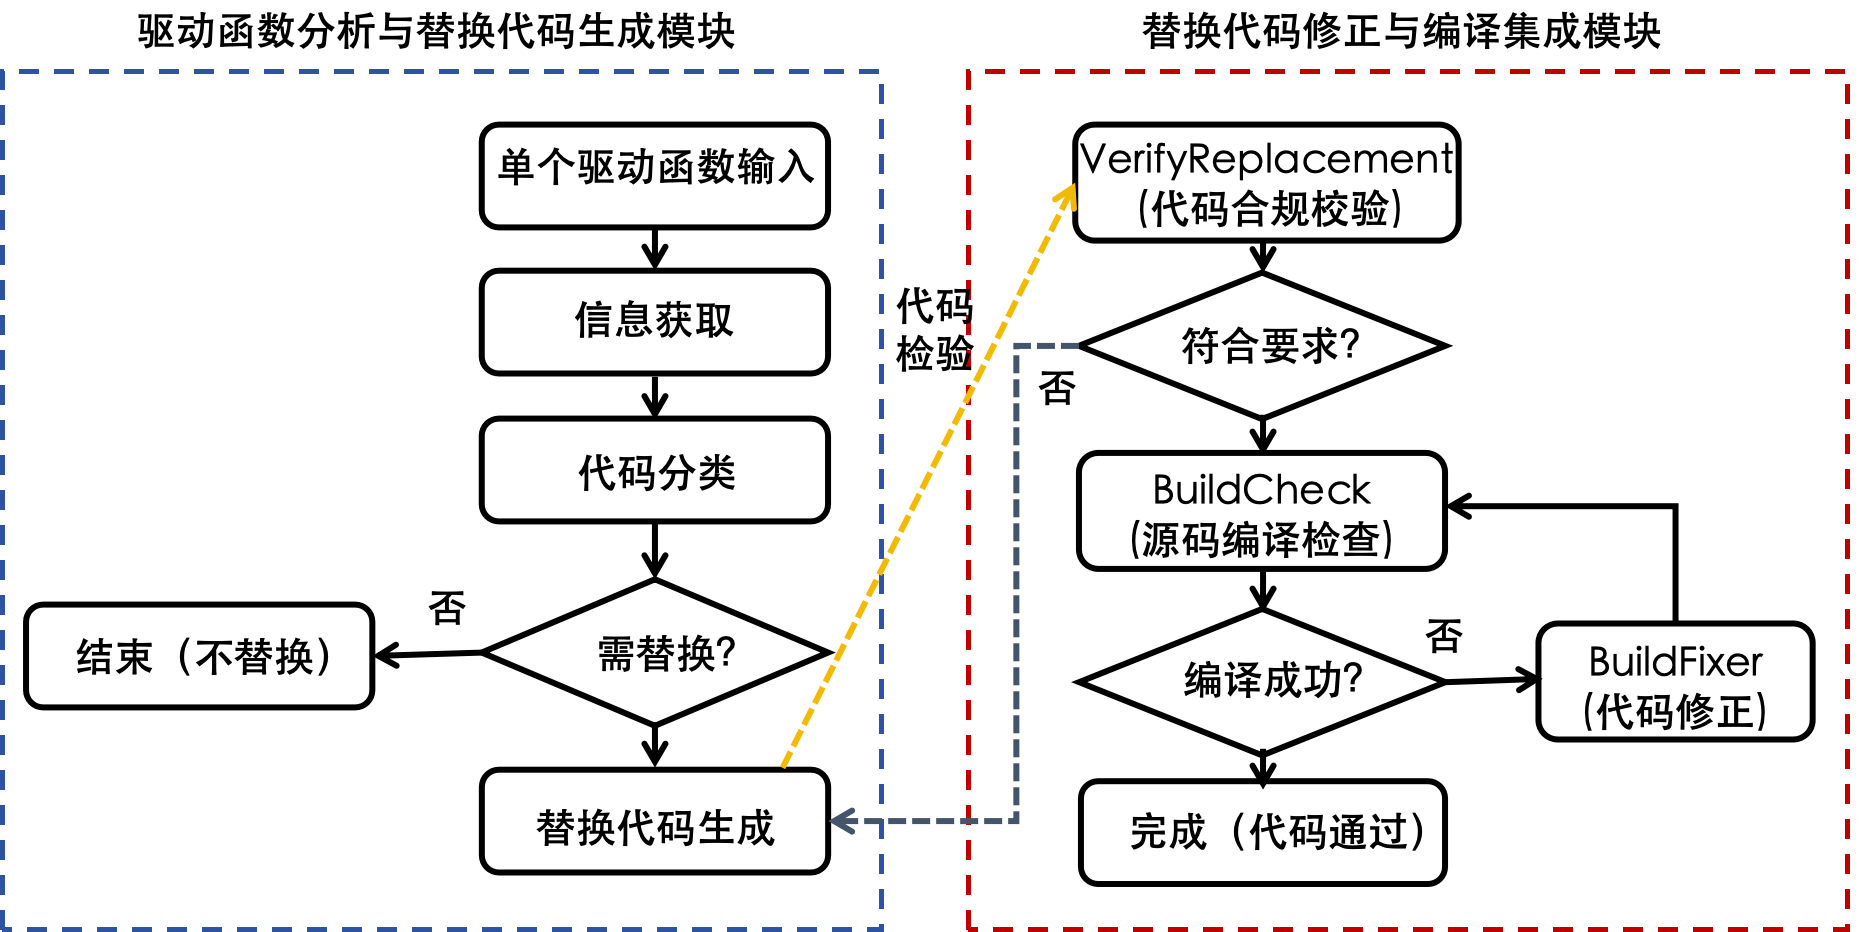
\includegraphics[width=\textwidth]{figures/驱动函数分析替换与编译.png}
    \caption{驱动函数分析替换编译模块示意图}
    \label{fig:analyzer-workflow}
\end{figure}

\subsubsection{驱动函数分析与替换代码生成模块设计}
\label{sec:analyzer-workflow}

该子模块由\textbf{分析智能体}驱动，在 LangGraph 状态机中通过"工具调用—推理—写回"的循环完成单函数处理。执行顺序固定为：\textbf{信息获取} $\to$ \textbf{代码分类} $\to$（仅在分类结果认定该函数需要替换时）\textbf{替换代码生成}。

\textbf{信息获取}阶段通过工具调用获取该驱动函数在工程中的完整上下文，包括完整实现或相关片段、函数签名与参数类型、调用关系与 MMIO 仿真侧提示等（如 GetFunctionInfo、GetFunctionCallStack、GetMMIOFunctionEmulateInfo）。\textbf{代码分类}阶段综合源码与静态分析结果，由大语言模型判定函数语义类别及是否属于必须替换的硬件相关行为；分类所依据的类别体系及提示构造方式见第~\ref{sec:driver-replacement-strategy}~节。\textbf{替换代码生成}仅在"需要替换"分支上触发：模型在既定类别上选择替换策略并产出与签名一致的候选实现，具体策略（如 Skip、Strip、Redirect、Event 等）的选择规则与生成约束同样在第~\ref{sec:driver-replacement-strategy}~节展开，本节只给出子模块内的先后次序与数据交接关系。

\subsubsection{替换代码修正与编译集成模块设计}
\label{sec:builder-workflow}

该子模块在工程目录中对上一子模块输出的\textbf{候选替换代码}做\textbf{二阶段检验与修复}，目标是在真实构建环境下得到可链接、可编译的替换定义。

\textbf{第一阶段（代码合规校验）}调用 VerifyReplacement，依据预置规则与接口契约检查候选替换是否满足替换定义（例如签名一致、禁止引入不兼容的存储类或明显违背仿真假设的写法等），过滤与定义明显不符的实现；未通过时可将反馈交回分析智能体侧重新生成或局部修订（图~\ref{fig:analyzer-workflow}中以虚线表示返回替换生成环节）。

\textbf{第二阶段（语法编译检查）}在通过定义校验后，将替换写入目标源文件（如 ReplaceFuncs，并保留回滚所需的原定义快照），再调用工程构建脚本执行完整编译链接（如 BuildProject）。若\textbf{编译失败}，则进入编译修复智能体路径：由编译修复智能体解析编译器诊断信息，结合 GetFunctionInfo、GetMMIOFunctionInfo 等工具定位首个关键错误，通过 UpdateFunctionReplacement 或 FixFunctionBuildErrors 等动作修订替换代码，并再次触发构建，形成"编译 $\to$ 错误解析 $\to$ 修复 $\to$ 重新编译"的闭环，直至编译成功或达到步数上限，从而保证最终被采纳的替换函数能够通过工程编译。

编译错误的典型成因包括函数未声明、类型不匹配、缺少头文件、链接错误，以及替换代码引用了目标芯片 HAL 中不存在的结构体成员或与头文件声明不一致等。例如，STM32F401 的 TIM\_HandleTypeDef 无 ErrorCode 成员、RCC\_PLLInitTypeDef 无 PLLR 成员时，若替换体仍访问这些成员会导致编译失败；将非静态函数误写为 static 亦会破坏链接一致性。编译修复智能体针对不同诊断采取补声明、改类型与转换、补 \texttt{\#include}、删改非法成员访问、核对依赖等策略。提示词上约束智能体在构建失败时优先根据 stderr 锁定\textbf{第一个错误}所涉函数再查上下文，避免对多函数无序轮询而浪费工具调用次数，从而兼顾修复质量与效率。

\subsection{驱动函数替换策略设计}
\label{sec:driver-replacement-strategy}

为实现语义保持的驱动函数替换，本研究在替换前先对驱动函数进行语义分类，并基于分类结果选择对应替换策略，避免硬件依赖被误删或替换不足导致仿真异常。

\subsubsection{函数分类策略设计}

驱动函数替换的核心挑战在于不同类型的驱动函数与硬件交互的方式和语义要求存在显著差异。采用无差别的统一替换策略无法准确处理各类函数的特殊性，容易导致仿真异常或语义丢失。因此，系统在替换前先对驱动函数进行语义分类，根据函数类别选择最合适的替换策略，从而确保替换后代码的正确性和仿真环境的稳定性。

系统基于大语言模型实现驱动函数的自动分类。LLM 通过读取函数源码、识别 MMIO 访问模式、判断函数主要用途等步骤，将函数分类到预定义的类别。分类策略基于对嵌入式驱动函数硬件交互模式的分析，将函数划分为以下类别，如表~\ref{tab:function-categories}所示。

设驱动函数集合 $D$ 上的分类映射定义为：
$$\textit{classify}: D \to C = \{\textit{INIT}, \textit{RECV}, \textit{LOOP}, \textit{IRQ}, \textit{RETURNOK}, \textit{SKIP}, \textit{CORE}, \textit{NODRIVER}\}$$

对于需要替换的函数子集 $D_r = \{f \in D \mid \textit{classify}(f) \in C \setminus \{\textit{CORE}, \textit{NODRIVER}\}\}$，系统进一步为其分配替换策略。替换策略映射定义为：
$$\textit{strategy}: D_r \to S = \{\textit{Skip}, \textit{Redirect}, \textit{Event}, \textit{Steering}, \textit{ReturnOK}\}$$

该分类体系旨在解决已有方法中替换策略与函数语义不匹配的问题。HALucinator~\cite{clements2020halucinator} 采用统一的 HAL profile 拦截策略，P2IM~\cite{fengp2020p2im} 通过随机 fuzzing 生成外设响应，均未对驱动函数的语义类别进行系统性区分。当替换策略与函数语义不匹配时，容易出现仿真异常——例如 LOOP 类函数未移除轮询逻辑引发死循环、RECV 类函数未注入模拟数据导致上层协议栈读取到无效值。本研究通过"先分类后替换"的范式，使每类函数获得与其语义特征相匹配的替换策略，从设计层面降低了替换导致的语义错误风险。

\subsubsection{分类判定规则}

为提高分类的准确性和一致性，系统为每类函数定义了明确的判定规则，LLM 在分类时需综合以下特征进行判定：

\textbf{（1）INIT 类判定规则}。满足以下条件之一的函数归类为 INIT：函数名包含 \texttt{Init}、\texttt{Config}、\texttt{Setup}、\texttt{MspInit} 等关键词；函数体内包含对多个 MMIO 寄存器的顺序写操作且无读-改-写循环；函数调用位置位于系统启动阶段或外设初始化流程中（通过调用图判断）。INIT 类函数的特征是对硬件进行一次性配置，执行后不依赖返回的硬件状态。

\textbf{（2）RECV 类判定规则}。满足以下条件之一的函数归类为 RECV：函数名包含 \texttt{Receive}、\texttt{Read}、\texttt{Get}、\texttt{Input} 等关键词；函数体内包含从 MMIO 数据寄存器（如 \texttt{RDR}、\texttt{DR}、\texttt{RXDATA}）的读操作；函数参数中包含目标缓冲区指针和长度参数。RECV 类函数的核心语义是从硬件获取数据并传递给上层软件，替换时需要通过仿真注入接口提供模拟数据。

\textbf{（3）LOOP 类判定规则}。满足以下条件之一的函数归类为 LOOP：函数名包含 \texttt{Wait}、\texttt{Poll}、\texttt{Loop} 等关键词；函数体内包含以 MMIO 状态寄存器（如 \texttt{ISR}、\texttt{SR}）的某一位为条件的循环结构（\texttt{while(flag == RESET)} 形式）；循环体内部无实质性的数据处理逻辑，仅为等待硬件状态变化。LOOP 类函数在仿真环境中会造成死循环，必须通过 Skip 策略移除等待逻辑。

\textbf{（4）IRQ 类判定规则}。满足以下条件之一的函数归类为 IRQ：函数名包含 \texttt{IRQHandler}、\texttt{Callback}、\texttt{Handler} 等关键词；函数被注册为中断服务例程（通过中断向量表或 \texttt{HAL\_RegisterCallback} 等方式）；函数体内包含对 MMIO 中断状态寄存器的读操作和清标志操作。IRQ 类函数的触发依赖硬件中断信号，在仿真环境中需要通过 Event 策略将其改造为可由仿真器主动触发的事件处理函数。

\textbf{（5）RETURNOK 类判定规则}。满足以下条件之一的函数归类为 RETURNOK：函数仅包含单个或少量简单的 MMIO 读操作且不使用读出值；函数的返回类型为状态枚举（如 \texttt{HAL\_StatusTypeDef}）且所有执行路径均返回成功状态；函数的语义等价于"检查硬件状态并返回成功"。RETURNOK 类函数在仿真环境中无需执行具体操作，直接返回成功状态值即可。

\textbf{（6）SKIP 类判定规则}。满足以下条件之一的函数归类为 SKIP：函数返回类型为 \texttt{void} 且函数体内的 MMIO 操作对固件状态机无影响；函数名包含 \texttt{DeInit}、\texttt{MspDeInit}、\texttt{Flush} 等资源释放类关键词；函数的功能仅为清理硬件状态或重置外设寄存器。SKIP 类函数在仿真环境中可以直接跳过执行。

\textbf{（7）CORE 类判定规则}。满足以下条件之一的函数归类为 CORE：函数属于操作系统内核代码（如 \texttt{rt\_thread\_init}、\texttt{SysTick\_Handler}）；函数的实现由仿真器直接提供，不经过替换流程。CORE 类函数由系统预配置，不参与 LLM 分类。

\textbf{（8）NODRIVER 类判定规则}。函数虽位于驱动模块中，但满足以下全部条件：函数体内不包含直接的 MMIO 寄存器访问；函数的功能为纯软件逻辑（如参数校验、错误码转换、辅助计算）；函数的执行不依赖任何硬件状态。NODRIVER 类函数在仿真环境中可直接运行，无需替换。

上述判定规则以结构化的形式嵌入 LLM 的分类提示模板中，指导模型从函数名、MMIO 访问模式、控制流结构和调用上下文四个维度综合判断，从而提高分类的一致性。当函数特征同时满足多个类别的判定条件时，LLM 根据函数的主要语义选择最合适的类别，优先级规则为：CORE > IRQ > RECV > LOOP > INIT > RETURNOK > SKIP > NODRIVER。

\begin{table}[htbp]
\centering
\caption{驱动函数分类体系}
\label{tab:function-categories}
\footnotesize
\setlength{\tabcolsep}{4pt}
\begin{tabular}{@{}llp{6.6cm}@{}}
\toprule
\textbf{缩写} & \textbf{描述} & \textbf{典型函数} \\
\midrule
INIT & 外设初始化，影响固件状态机 & \texttt{HAL\_UART\_Init}, \texttt{BOARD\_BootClockRUN} \\
RECV & 从硬件/DMA 读取数据 & \texttt{HAL\_UART\_Receive}, \texttt{ENET\_GetRxFrame} \\
LOOP & 轮询等待硬件状态 & \texttt{HAL\_UART\_WaitOnFlag}, \texttt{FLASH\_WaitForLastOperation} \\
IRQ & 中断处理/回调函数 & \texttt{HAL\_UART\_IRQHandler}, \texttt{ENET\_TransmitIRQHandler} \\
RETURNOK & 纯硬件操作，返回状态值 & \texttt{HAL\_GPIO\_DeInit}, \texttt{HAL\_I2C\_IsDeviceReady} \\
SKIP & 纯硬件操作，无返回值 & \texttt{HAL\_ADC\_MspInit}, \texttt{FLASH\_FlushCaches} \\
\midrule
CORE & 系统区操作，OS 核心函数 & \texttt{SysTick\_Handler}, \texttt{rt\_thread\_init} \\
NODRIVER & 存在的驱动操作对固件状态机无影响 & \texttt{main}, \texttt{GPIO\_GetInstance} \\
\bottomrule
\end{tabular}
\end{table}

这八类函数覆盖了嵌入式固件中与硬件交互的各种典型模式。其中，INIT、RECV、LOOP、IRQ、RETURNOK 和 SKIP 六类函数均直接或间接地涉及 MMIO 寄存器访问，需要通过替换消除硬件依赖；CORE 类函数涉及操作系统核心功能（如系统定时器、线程调度），由仿真器直接提供底层支持，无需替换；NODRIVER 类函数虽然存在于驱动模块中，但其操作对固件状态机无影响或属于纯业务逻辑，同样无需替换。该分类体系的设计兼顾了完备性和实用性，确保每类函数都有明确的替换策略或处理方式。

\subsubsection{替换策略体系设计}

本研究总结出五种通用替换策略，每种策略适用于特定的函数类别和使用场景。表~\ref{tab:replace-strategies}展示了各类函数与替换策略的对应关系，策略的选择由 LLM 根据函数的语义特征自动决定。

\begin{table}[htbp]
\centering
\caption{替换策略选择指南}
\label{tab:replace-strategies}
\footnotesize
\setlength{\tabcolsep}{4pt}
\begin{tabular}{@{}llp{5.9cm}@{}}
\toprule
\textbf{函数类别} & \textbf{策略类型} & \textbf{说明} \\
\midrule
INIT & Skip/Steering & 移除硬件寄存器操作，保留结构体初始化，避免仿真环境中的阻塞 \\
RECV & Redirect/Steering & 利用 HAL\_BE\_* 注入函数重定向输入输出，实现数据注入 \\
LOOP & Skip & 移除轮询等待逻辑，避免仿真环境中的死循环，直接返回成功状态 \\
IRQ & Event & 保留回调函数签名，直接触发事件通知，移除硬件条件判断 \\
RETURNOK & ReturnOK & 直接返回成功状态值，保留函数签名，不执行硬件操作 \\
SKIP & Skip & 直接跳过函数执行，保留函数签名和调用路径，函数体为空 \\
\midrule
CORE & NoReplacement & 完全不替换，保留原函数代码和调用关系，由仿真器提供底层支持 \\
NODRIVER & NoReplacement & 不进行任何替换，保留原函数代码和调用关系 \\
\bottomrule
\end{tabular}
\end{table}

以下逐一阐述各策略的设计原理和适用场景。

\textbf{Skip 策略}：移除硬件交互操作。Skip 策略移除驱动函数中的硬件交互操作，但保留函数签名和返回值，使函数执行路径能够支持固件正常运行。对于初始化类函数，移除硬件寄存器配置逻辑；对于控制类函数，移除控制命令的硬件执行；对于轮询类函数，移除等待硬件状态的循环逻辑，避免仿真环境中的死循环。Skip 策略跳过与硬件相关的操作，保留了必要的返回值和函数接口，避免固件因硬件依赖而阻塞或异常。

\textbf{Redirect 策略}：重定向到仿真 I/O。Redirect 策略使用自定义的注入函数（如 HAL\_BE\_In、HAL\_BE\_ENET\_ReadFrame、HAL\_BE\_Out）替代硬件访问，为替换后的驱动代码提供与仿真环境交互的标准接口。对于接收类函数，使用 HAL\_BE\_In（固定长度）或 HAL\_BE\_ENET\_ReadFrame（变长报文）将仿真输入数据填充到缓冲区；对于发送类函数，使用 HAL\_BE\_Out 重定向输出或在不影响状态时跳过写操作。

\textbf{Event 策略}：事件驱动模拟。Event 策略通过事件队列模拟硬件中断触发。在仿真环境中，硬件中断信号由仿真器生成的事件触发，而非真实的硬件信号。该策略保留中断处理函数中的数据处理和回调触发逻辑，移除硬件中断标志寄存器的操作，通过控制流改写让中断处理函数必然执行到 OS 通知和回调触发分支。

\textbf{Steering 策略}：执行流导向。Steering 策略通过控制流旁路和改写，将因硬件依赖而不可达的执行路径导向到仿真可达且语义保持的分支。该策略适用于依赖硬件标志的循环、基于 DMA+RingBuffer 的数据接收状态机等复杂场景。当固件因为硬件依赖导致执行路径不可达时，Steering 策略改写控制流把执行导向到仿真可用的路径，同时保证数据传输和状态更新的语义一致性。

\textbf{ReturnOK 策略}：直接返回成功。ReturnOK 策略针对 RETURNOK 类函数，这类函数通常是简单的辅助函数，主要功能是设置状态、清理资源或执行简单的检查。该策略保留函数签名和必要的参数校验，删除函数体的具体实现，直接返回成功状态（如 HAL\_OK）。

\textbf{与已有方法替换策略的差异}。已有固件仿真方法在处理硬件依赖时主要采用两种策略：一是 HALucinator~\cite{clements2020halucinator} 通过手工编写 HAL profile 来拦截和替换函数调用，该方法依赖领域专家针对每种芯片平台逐一手动编写适配规则，可扩展性有限；二是 P2IM~\cite{fengp2020p2im} 和 Pretender~\cite{pretender} 采用随机或学习策略生成外设响应，在运行时通过 fuzzing 方式探索外设行为空间，但随机生成的响应可能导致固件执行偏离正常路径。本系统采用的"先分类后替换"策略具有三点优势：（1）通过语义分类识别函数的硬件交互模式，针对性地选择替换策略，避免了"一刀切"替换导致的语义丢失；（2）利用 LLM 的代码理解能力自动生成替换代码，无需针对每种芯片平台手动编写适配规则；（3）通过 Redirect 和 Steering 等策略提供结构化的数据注入机制，相比随机响应更能保证固件执行路径的语义正确性。

\subsection{替换验证机制设计}

替换代码生成后，需要在实际集成到固件工程之前进行严格的质量检查。由于替换代码由大语言模型生成，可能存在语法错误、签名不一致或语义偏移等问题，若未经校验直接写入工程，将导致编译失败或运行时异常。因此，系统设计了多层验证机制，在代码写入工程前尽可能拦截不合格的替换实现，减少后续编译修复的迭代次数，提高整体效率。

系统对生成的替换代码进行以下四层验证：

设原始函数为 $f$，生成的替换函数为 $f'$，替换函数的替换代码为 $\textit{code}(f')$。四层验证的形式化定义如下：

（1）\textbf{语法正确性检查}：验证 $\textit{code}(f')$ 的语法结构完整性：
$$V_1(f') = \textit{syntax\_valid}(\textit{code}(f'))$$

（2）\textbf{签名匹配检查}：验证替换函数签名与原始函数完全一致：
$$V_2(f') = (\textit{sig}(f') = \textit{sig}(f))$$
其中 $\textit{sig}(f) = (\textit{name}(f), \textit{ret\_type}(f), \textit{params}(f))$ 表示函数签名三元组。

（3）\textbf{返回值检查}：验证所有执行路径的返回值与返回类型一致：
$$V_3(f') = \forall\, \pi \in \textit{paths}(f'): \textit{ret\_value}(\pi, f') \in \textit{ret\_domain}(f)$$
其中 $\textit{paths}(f')$ 表示函数 $f'$ 中从入口到出口的所有执行路径。

（4）\textbf{替换规则检查}：验证替换代码遵守策略约束条件：
$$V_4(f') = \textit{rule\_check}(\textit{code}(f'), \textit{strategy}(f'))$$

替换函数通过验证当且仅当四层检查全部通过：
$$\textit{valid}(f') = V_1(f') \wedge V_2(f') \wedge V_3(f') \wedge V_4(f')$$

\subsubsection{语义保持性定义}

替换验证的目标是确保替换代码在仿真环境中保持原始函数的业务语义。由于驱动函数的语义由其与固件其他部分的交互决定，语义保持性无法仅通过静态分析完全验证，需要通过动态测试闭环进一步确认。本研究将语义保持性定义为以下约束条件：

设原始驱动函数 $f$ 的语义为 $\mathcal{S}(f)$，替换函数 $f'$ 的语义为 $\mathcal{S}(f')$。语义保持性要求替换后的固件工程 $P'$ 在仿真环境中满足以下条件：

\textbf{（1）控制流可达性}：设 $B(P)$ 为固件工程 $P$ 中从入口到各关键节点（如 \texttt{main} 函数入口、RTOS 内核启动点、协议栈初始化完成点）的执行路径集合，则：
$$\forall\, \pi \in B(P_{\textit{target}}): \exists\, \pi' \in B(P'): \textit{key\_nodes}(\pi') \supseteq \textit{key\_nodes}(\pi)$$
其中 $P_{\textit{target}}$ 为目标执行路径集，$\textit{key\_nodes}(\pi)$ 表示路径 $\pi$ 上的关键节点集合。该条件确保固件在替换后仍能到达所有关键执行节点。

\textbf{（2）状态一致性}：设 $\Sigma$ 为固件状态空间，$\sigma_0 \in \Sigma$ 为初始状态，$\textit{step}(P, \sigma)$ 为固件执行一步的状态转移函数。对于固件中不受替换影响的软件模块（如操作系统调度器、协议栈逻辑），其可观测状态在替换前后应保持一致：
$$\forall\, m \in M_{\textit{soft}}: \textit{obs}(\textit{step}^*(P, \sigma_0), m) = \textit{obs}(\textit{step}^*(P', \sigma_0), m)$$
其中 $M_{\textit{soft}}$ 为纯软件模块集合，$\textit{obs}(\sigma, m)$ 为对模块 $m$ 的可观测状态提取函数，$\textit{step}^*$ 表示多步执行。

\textbf{（3）接口兼容性}：替换函数 $f'$ 对调用方的可观测行为应与原始函数 $f$ 一致，包括返回值类型正确、参数列表不变、对非硬件相关的全局状态的副作用保持一致：
$$\forall\, c \in \textit{callers}(f): \textit{contract}(f', c) = \textit{contract}(f, c)$$
其中 $\textit{contract}(f, c)$ 表示函数 $f$ 对调用方 $c$ 的行为契约（返回值、参数副作用）。

这三个条件共同构成替换的语义保持性要求。控制流可达性通过动态测试验证——仿真运行时检查固件是否到达预设的关键节点；状态一致性通过仿真运行中的状态采集和比对验证；接口兼容性通过前述四层静态验证（$V_1 \wedge V_2 \wedge V_3 \wedge V_4$）和动态测试联合保障。由于语义保持性无法通过纯静态分析完全保证，系统设计了"静态验证$\to$动态测试$\to$反馈修正"的多层保障机制，通过迭代闭环逐步满足语义保持性要求。

这四层验证形成层次化的质量过滤机制：语法检查过滤最基本的格式错误，签名和返回值检查确保函数接口的一致性，替换规则检查验证替换策略的执行规范性。未通过验证的替换代码将被退回分析智能体重新生成，并附上具体的错误描述，以便 LLM 在下一轮生成中针对性地修正问题。

\section{动态测试反馈闭环模块设计}

动态测试反馈闭环模块是连接"代码替换"与"仿真验证"的关键环节，负责将经过静态分析和替换处理的固件部署到仿真平台中执行，通过实际运行检验替换代码的正确性，并将运行过程中发现的错误进行迭代修复。已有固件仿真方法在验证环节普遍存在不足：P2IM~\cite{fengp2020p2im} 和 Pretender~\cite{pretender} 通过 fuzzing 反馈优化外设响应生成，但其反馈目标是改进随机策略的参数，而非修复固件本身的执行问题；HALucinator~\cite{clements2020halucinator} 依赖人工分析仿真失败原因并手动调整 HAL profile，缺乏自动化反馈机制。本研究提出编译错误与运行时错误的双层闭环修复机制：模块二中的编译修复智能体处理替换代码集成阶段的静态错误（语法错误、类型不匹配），模块三中的闭环修复智能体处理仿真运行阶段的动态错误（崩溃、死循环、语义偏差），两层闭环通过仿真执行智能体统一调度，实现了从静态替换到动态验证的全自动化。本系统设计了"运行→诊断→修复→回归"的自动化闭环：首先在基于 Unicorn 引擎的仿真平台上加载并执行替换后的固件，通过多种钩子机制全面采集指令执行、基本块覆盖、函数调用和中断触发等运行时信息；当仿真运行出现崩溃、死循环或内存异常等错误时，仿真执行智能体自动分析运行日志定位问题函数，触发闭环修复智能体生成修复方案，修复后重新构建并再次运行仿真，直至固件能够正常完成执行或达到最大迭代次数。本节依次阐述动态执行环境设计、仿真执行智能体设计、反馈信息结构化设计和迭代优化机制设计。

\subsection{动态执行环境设计}

\subsubsection{仿真平台架构设计}

系统采用基于 Unicorn 引擎的固件仿真框架进行动态测试。在仿真平台的选型上，本模块选择 Unicorn 而非 QEMU，主要基于以下理由。Firmadyne~\cite{firmadyne} 和 HALucinator~\cite{clements2020halucinator} 等系统基于 QEMU 构建仿真环境，QEMU 提供了完整的外设模型和操作系统支持，适合运行基于 Linux 的固件，但对于裸机固件而言，QEMU 的设备模型过于重量级，且难以精确控制函数级别的执行拦截。Unicorn 是库级别的 CPU 模拟器，支持 ARM Thumb 模式，可以直接执行 Cortex-M 固件；同时提供细粒度的 Hook 机制（指令级、基本块级、内存访问级），可以在执行过程中拦截注入函数调用并转移至宿主机侧处理。P2IM~\cite{fengp2020p2im} 同样基于 Unicorn 构建仿真平台，验证了 Unicorn 在裸机固件仿真场景中的适用性，但 P2IM 采用随机生成策略模拟外设响应，而本系统通过驱动函数替换和结构化数据注入实现更精确的仿真。

固件仿真子模块采用双层架构设计，由\textbf{仿真引擎层}与\textbf{Hook 机制层}构成。仿真引擎层负责提供指令集执行、内存映射等基础仿真能力；Hook 机制层则在指令流和访存路径上设置回调机制，实现函数入口的拦截和宿主侧逻辑的调用，从而支持驱动替换后注入接口的执行。

仿真引擎层基于 Unicorn ARM 模拟器实现 ARMv7-M Thumb 指令集的模拟执行，包括寄存器管理、内存访问以及固件映像的加载和地址空间映射配置。

Hook 机制层通过代码 Hook、基本块 Hook、内存读/写 Hook 和中断 Hook 等机制，实现执行过程中的信息采集和干预。该机制主要用于代码覆盖率统计、异常内存访问检测和执行轨迹记录等分析任务。在与替换策略配套时，Hook 机制层承担了关键作用：通过预留 \texttt{HAL\_BE\_*} 系列注入接口进行函数入口级拦截。具体而言，链接阶段的弱符号桩在宿主机侧被接管，当执行流到达约定入口时，不再在模拟 CPU 上执行原函数体，而是转入宿主机例程，完成缓冲区读写、数据帧搬运或块传输等操作，并按照调用约定返回结果和更新内存状态，随后继续执行。通过这种方式，驱动函数使用 Redirect 策略写入固件的 \texttt{HAL\_BE\_*} 接口调用可以被固件仿真模块拦截并执行，以支持固件与仿真平台的数据交互，完成固件与仿真平台的协同工作。

表~\ref{tab:hal-be-hooks}归纳\textbf{固件仿真模块}中与驱动替换配套的注入接口及其使用场景。

\begin{table}[htbp]
\centering
\caption{固件仿真模块注入接口与使用场景}
\label{tab:hal-be-hooks}
\footnotesize
\setlength{\tabcolsep}{5pt}
\renewcommand{\arraystretch}{1.15}
\begin{tabular}{@{}>{\raggedright\arraybackslash}p{5.05cm}p{7.7cm}@{}}
\toprule
\textbf{注入接口} & \textbf{使用场景} \\
\midrule
\texttt{HAL\_BE\_return\_0} & 恒定返回 0，多用作成功码或空操作占位；替换侧用于仅需固定"成功"语义、无需真实硬件操作。 \\
\texttt{HAL\_BE\_return\_1} & 恒定返回 1，多用作布尔真或约定非零语义。 \\
\texttt{HAL\_BE\_Out} & 以输出长度表征一次发送语义，常见于类 SEND 的 输出重定向策略。 \\
\texttt{HAL\_BE\_In} & 定长接收：将仿真输入写入缓冲区，常见于类 RECV 的 输入重定向策略。 \\
\texttt{HAL\_BE\_ENET\_ReadFrame} & 在变长上界内填充一帧网络类数据，常见于类 RECV 的 输入重定向策略。 \\
\texttt{HAL\_BE\_Block\_Read} & 按块大小与块数从虚拟介质读入缓冲区，常见于存储或块设备类替换。 \\
\texttt{HAL\_BE\_Block\_Write} & 按块粒度写出缓冲区内容，常见于块设备或大块 I/O 类替换。 \\
\bottomrule
\end{tabular}
\end{table}

\subsection{仿真执行智能体设计}

本节设计仿真运行主控智能体（Emulator Runner Agent），该智能体作为动态测试反馈闭环的核心调度单元，负责在仿真环境中执行固件并采集运行日志、崩溃信息等执行数据。为行文简洁，下文将仿真运行主控智能体简称为"仿真智能体"。

\subsubsection{职责定义与工具链设计}

仿真智能体的核心职责包括以下五个方面：（1）启动仿真运行并实时监控执行状态；（2）分析仿真输出并判断运行是否成功；（3）在运行失败时触发故障诊断，定位问题函数；（4）在修复完成后调用闭环构建智能体重新构建；（5）执行回归验证并判断是否需要继续迭代。为实现上述职责，该智能体绑定了三类工具：仿真执行工具（EmulateProject），用于启动固件仿真并采集运行结果；信息查询工具（GetMMIOFunctionEmulateInfo、GetFunctionCallsEmulateInfo），用于获取 MMIO 函数调用日志和函数调用栈信息，支撑故障诊断；以及修复工具和构建工具，通过工具调用接口与闭环修复智能体和闭环构建智能体交互。

\subsubsection{决策逻辑设计}

仿真智能体的决策逻辑由大语言模型（LLM）驱动，采用条件分支的状态机模型。LLM 根据当前仿真运行的状态和日志信息，在以下决策点进行判断：（1）仿真结果评估——根据退出码、异常循环检测标志等判断运行是否成功，若成功则终止闭环并返回结果；（2）修复需求判断——根据标准输出和标准错误中的错误信息，判断是否需要调用闭环修复智能体进行修复；（3）构建触发判断——在修复完成后，判断是否需要触发闭环构建智能体执行重新编译；（4）迭代终止判断——根据当前迭代轮次与最大迭代次数限制的比较结果，决定继续迭代或终止闭环并返回失败报告。该决策机制使得智能体能够根据运行时状态自主调整执行路径，而非依赖预定义的固定流程。

\subsubsection{仿真执行流程设计}

仿真智能体的仿真执行流程分为四个阶段。首先为环境准备阶段，仿真智能体根据目标固件的硬件平台配置 CPU 架构模式和内存映射，包括设置程序计数器（PC）和栈指针（SP）的初始值，以及加载链接脚本和中断向量表等配置信息。其次为固件加载阶段，仿真智能体将编译生成的 ELF 文件加载到 Unicorn 引擎的虚拟内存空间中，完成符号解析和地址重定位。第三为执行监控阶段，仿真智能体启动仿真器运行固件，通过指令级 Hook 和内存访问 Hook 实时采集运行日志、程序计数器变化和内存访问记录，同时监控异常信号（如段错误、非法指令）和运行超时情况。第四为结果分析阶段，仿真智能体对采集的日志和状态信息进行综合分析，判断运行是否成功，若失败则提取崩溃地址、错误类型和调用栈等关键信息，生成结构化的反馈摘要传递给故障诊断模块。

\subsection{反馈信息结构化设计}

系统在仿真运行过程中采集多种类型的运行信息，用于评估替换效果和指导迭代优化。运行监控采集的信息包括执行状态（成功、失败、超时）、程序计数器的最终值、执行的基本块数量、执行的指令总数、标准输出和标准错误输出等。系统定义了统一的数据结构来表示执行结果，包含上述所有采集的信息，该数据结构作为动态测试反馈模块的输出传递给上游模块。

覆盖率统计用于评估固件代码的执行覆盖程度，系统支持基本块级覆盖率统计，通过块 Hook 记录执行过程中访问的所有基本块的地址。错误分类系统将运行过程中发生的各种错误按照类型进行分类，包括执行崩溃错误（访问无效内存、执行非法指令等）、执行超时错误（死循环、阻塞等待等）以及外设或 MMIO 访问相关的异常。

仿真运行产生的原始日志通常是大量的非结构化文本信息，系统对原始日志进行结构化处理，提取关键信息形成反馈摘要。反馈摘要包含迭代轮次、失败类型、错误地址、崩溃信息、相关驱动函数列表和修复建议等字段。反馈信息结构化处理流程包括日志解析、关键信息提取、相关驱动函数分析和摘要生成四个阶段，通过调用栈分析确定错误发生时正在执行的驱动函数及其调用链。

\subsection{迭代优化机制设计}

当运行失败时，闭环修复智能体被触发进行针对性修复。需要指出的是，闭环修复智能体与模块二中的编译修复智能体职责不同：编译修复智能体处理替换代码首次集成时的编译错误（如语法错误、类型不匹配等静态问题），闭环修复智能体处理仿真运行时发现的动态错误（如崩溃、死循环、语义偏差等运行时问题），两类错误的诊断方式和修复策略存在本质差异。设第 $i$ 轮迭代的状态为 $S_i = (P_i, E_i)$，其中 $P_i$ 为当前固件工程，$E_i$ 为仿真运行产生的错误集合。闭环修复过程定义为状态转移序列：
\begin{align}
S_0 &= (P_0, E_0) \nonumber \\
S_{i+1} &= \begin{cases}
(P_i, \emptyset) & \text{if } E_i = \emptyset \quad \textit{(成功终止)} \\
\textit{Fix}(P_i, E_i) & \text{if } E_i \neq \emptyset \land i < K \land \neg\textit{stagnant}(i) \quad \textit{(继续修复)} \\
S_i & \text{otherwise} \quad \textit{(失败终止)}
\end{cases} \label{eq:iterate}
\end{align}
其中 $K$ 为最大迭代次数，$\textit{Fix}(P_i, E_i)$ 表示对工程 $P_i$ 施加基于错误 $E_i$ 的修复操作，$\textit{stagnant}(i)$ 表示连续 $N$ 轮迭代未能引入新的修复。修复操作包括以下步骤：

\subsubsection{错误诊断算法设计}

系统采用基于规则与大语言模型相结合的错误诊断算法，根据运行失败的类型选择相应的诊断策略：

\textbf{编译错误诊断}。编译错误的诊断信息由编译器直接提供（如 \texttt{error: unknown type name}、\texttt{warning: implicit declaration}），系统通过正则表达式从编译器输出中提取错误类型、源文件路径和行号，精确定位到具体的替换函数和出错语句。诊断算法优先锁定编译器报告的第一个错误，原因在于后续错误往往由首个错误的连锁反应引起，修复首个错误后重新编译可大幅减少需要处理的错误数量。

\textbf{运行崩溃诊断}。运行崩溃由 Unicorn 引擎捕获的异常信号触发，常见类型包括访问无效内存地址（如 \texttt{SIGSEGV}）、执行非法指令（如 \texttt{SIGILL}）和栈溢出等。诊断算法从崩溃现场提取以下信息：程序计数器（PC）的值、触发崩溃的指令地址、当前函数调用栈和崩溃时的寄存器状态。通过将崩溃地址与静态分析模块输出的函数地址范围进行比对，确定崩溃发生在哪个替换函数内部还是固件业务逻辑中。若崩溃发生在替换函数内部，则直接定位到该函数进行修复；若崩溃发生在业务逻辑中，则通过调用栈分析追溯到最近一次调用的替换函数，判断是否因替换不当导致传入参数异常。

\textbf{运行超时诊断}。运行超时由预设的执行时间上限或指令数上限触发，通常表明固件进入了死循环或阻塞等待状态。诊断算法通过分析超时时刻的程序计数器分布，识别反复执行的指令区间和对应的循环结构，判断超时是否由未被替换的轮询类驱动函数引起。若确认为 LOOP 类函数未被正确替换，则触发该函数的重新分析和替换。

\subsubsection{迭代终止条件}

系统的迭代优化过程设置以下终止条件，确保闭环不会无限运行：

\textbf{成功终止条件}。当仿真运行满足以下全部条件时终止迭代：固件执行到预设的关键节点（如 \texttt{main} 函数入口、RTOS 内核启动、协议栈初始化完成等）；仿真运行过程中未发生崩溃或超时；替换代码通过编译验证且无编译器警告。

\textbf{失败终止条件}。当满足以下任一条件时终止迭代并输出失败报告：连续 $N$ 轮迭代未能引入新的修复（$N$ 的默认值为 3），表明当前错误已超出自动修复能力；迭代轮次达到预设的最大迭代次数上限（默认值为 10），防止过长时间占用计算资源；诊断算法判断错误类型为不可自动修复的类别（如固件依赖的第三方库函数缺失、链接器脚本配置错误等）。

通过"静态分析 $\to$ 智能替换 $\to$ 编译验证 $\to$ 动态测试 $\to$ 反馈优化"的完整闭环，系统不断迭代优化替换策略。

\section{本章小结}

本章围绕"基于驱动程序替换的固件仿真"给出了系统级设计方案。系统采用"静态识别 $\to$ 智能替换 $\to$ 构建验证 $\to$ 动态反馈"的分层模块化架构，各模块职责分工和数据流关系如第~\ref{chap:design}~节所述。在此基础上，本章分别完成了三个核心模块的设计：

\textbf{（1）静态分析模块设计}：提出了基于 CodeQL 污点追踪的 MMIO 访问模式识别方法，形式化定义了直接地址强转、间接初始化和常量指针参数三种定位模式，设计了驱动函数定位准则和数据流追踪方法，构建了统一的数据模型。

\textbf{（2）替换模块设计}：提出了基于语义分类的驱动函数替换方法，构建了涵盖八类函数的分类体系和五种对应的替换策略，设计了四层验证机制和语义保持性定义，通过大语言模型驱动的智能体架构实现了分类和替换的自动化。

\textbf{（3）动态反馈模块设计}：设计了编译错误与运行时错误的双层闭环修复机制，基于 Unicorn 引擎构建了仿真平台，设计了仿真智能体和迭代优化流程，实现了"运行→诊断→修复→回归"的自动化闭环。

这三个模块协同工作，实现了"静态识别 $\to$ 智能替换 $\to$ 构建验证 $\to$ 动态反馈"的完整闭环。
  % 系统设计
\chapter{系统实现}
\label{chap:implementation}

\section{驱动函数接口静态分析与识别模块实现}

\subsection{CodeQL 查询实现}

查询流水线依次执行四阶段：MMIO 表达式收集 $\to$ 基址数据流追踪 $\to$ 驱动函数判定 $\to$ 调用关系查询，各阶段输出作为下一阶段输入。

\subsubsection{MMIO 操作定位查询实现}

针对三种 MMIO 定位模式，本研究设计了相应的查询规则。查询的核心设计思想是将"寄存器字段访问"追溯到一个可被 CodeQL 稳定描述的基对象表达式。代码~\ref{lst:mmio-collect}展示了 MMIO 表达式收集查询，通过 \texttt{import libraries.MMIOAnalyzer} 引入 MMIO 分析库，从数据库中提取所有符合条件的 MMIO 表达式及其所属函数、文件路径、行号和类型信息。

\begin{lstlisting}[style=CodeQL,language=CodeQL, caption={MMIO表达式收集查询示例},label=lst:mmio-collect]
import cpp
import libraries.MMIOAnalyzer

from Function func, InterestingMMIOExpr expr
where isInterestingMMIOFunction(func) and
     expr.getEnclosingFunction() = func
select expr.toString(),
       expr.getEnclosingFunction().getName(),
       expr.getFile().getAbsolutePath().toString(),
       expr.getLocation().getStartLine()
\end{lstlisting}

对于"间接初始化"和"基址直传"模式，查询采用 CodeQL 的数据流追踪能力，将外设基址常量（如 \texttt{USART1\_BASE}）作为源点，沿赋值语句和函数参数传播追踪到最终的字段解引用操作（如 \texttt{huart->Instance->DR}），如代码~\ref{lst:taint-tracking}所示。

\begin{lstlisting}[style=CodeQL,language=CodeQL, caption={常量基址数据流追踪查询示例},label=lst:taint-tracking]
predicate isMMIOTracedExpr(Expr e) {
    exists(DataFlow::Node source, DataFlow::Node sink,
           ConstantExpr src_mmio |
        source.asExpr() = src_mmio and
        isConstantBigValueExpr(src_mmio) and
        sink.asExpr() = e and
        TaintFlow::flow(source, sink) and
        not sink.asExpr().getFile() instanceof DriverFile
    )
}
\end{lstlisting}

对于"基址直传"模式，查询通过函数调用关系和参数类型匹配定位调用点：当函数的第 0 个参数类型为 MMIO 结构体指针且实参是经过数据流追踪的常量表达式时，该调用点即为候选的 MMIO 使用点。三种查询的结果经聚合后形成完整的 MMIO 使用链路，为驱动函数识别提供输入。

\subsubsection{驱动函数定位查询实现}

驱动函数定位的判定规则见第~\ref{sec:design-driver-loc}~节，其 CodeQL 实现如代码~\ref{lst:driver-function-rule}所示。MMIO 访问包括直接字段访问（\texttt{MMIOFieldAccess}）和间接字段访问（\texttt{DriverFieldAccess}），两类访问的函数均被识别为驱动函数。

\begin{lstlisting}[style=CodeQL,language=CodeQL, caption={驱动函数判定规则},label=lst:driver-function-rule]
class DriverFunction extends Function
{
    DriverFunction() {
        exists(DriverFieldAccess fa | fa.getEnclosingFunction() = this)
        or
        exists(MMIOFieldAccess fa | fa.getEnclosingFunction() = this)
    }
}
\end{lstlisting}

该查询定义了 \texttt{DriverFunction} 类，该类继承自 \texttt{Function}，通过检查函数内部是否包含 \texttt{DriverFieldAccess} 或 \texttt{MMIOFieldAccess} 来判定函数是否为驱动函数，与设计章中"凡是包含 MMIO 访问的函数均定义为驱动函数"的准则一致。

在识别出驱动函数列表后，模块进一步分析驱动函数之间的调用关系，构建函数调用图。调用图以驱动函数为节点，函数调用关系为边，记录调用方、被调用方、调用位置等信息。调用图记录了函数间的调用依赖关系，有助于理解函数的调用上下文和语义关联。

\begin{lstlisting}[style=CodeQL,language=CodeQL, caption={驱动函数调用关系查询},label=lst:driver-call-query]
from DriverToCall call
select call.toString2(),
       call.getTargetFunction().toString(),
       call.getEnclosingFunction().toString(),
       call.isDirectCall()
\end{lstlisting}

该查询从 \texttt{DriverToCall} 关系中提取驱动函数之间的调用关系，输出调用边的字符串表示、目标函数名、封装函数名以及调用是否为直接调用等信息，如代码~\ref{lst:driver-call-query}所示。

\subsection{数据模型实现}

为便于后续模块使用，静态分析结果被组织为统一的数据模型。数据模型采用 Python 数据类（dataclass）定义，支持序列化和反序列化，包括函数信息模型（\texttt{FunctionInfo}，包含函数名、签名、MMIO 访问列表等）、MMIO 访问点模型（\texttt{MmioAccessInfo}，包含结构体类型、字段名、访问类型等）和项目分析结果模型（包含调用图、驱动函数列表等），通过 JSON 序列化存储在缓存层供后续模块查询。

\subsubsection{查询工具函数实现}

各模块的数据通过一组工具函数对外暴露，供智能体在 LangGraph 工作流中调用。工具函数基于 LangChain 的 \texttt{@tool} 装饰器实现，将底层的数据查询封装为 LLM 可直接调用的工具接口。表~\ref{tab:tools}列出了系统中的主要工具函数及其功能。

\begin{table}[htbp]
\centering
\caption{主要工具函数}
\label{tab:tools}
\footnotesize
\setlength{\tabcolsep}{3pt}
\begin{tabular}{@{}lp{10.5cm}@{}}
\toprule
\textbf{工具函数} & \textbf{功能说明} \\
\midrule
GetFunctionInfo & 检索函数源码、签名、参数列表、返回类型、文件位置等信息 \\
GetMMIOFunctionInfo & 返回函数的所有 MMIO 访问点（结构体类型、字段名、访问类型、上下文代码） \\
GetFunctionCallStack & 提取函数的调用者列表和被调用者列表，返回调用关系双向视图 \\
GetStructOrEnumInfo & 查询数据结构或枚举类型的定义 \\
GetDriverInfo & 获取驱动模块的上下文信息 \\
\bottomrule
\end{tabular}
\end{table}

上述工具基于静态分析结果查询，内部实现了缓存机制避免重复访问。此外，系统还提供基于仿真运行结果的查询工具（如 MMIO 函数调用日志、函数调用栈信息），在仿真执行智能体中进行故障诊断时使用（见第~\ref{sec:hook-mechanism}~节）。各工具函数的返回结果均经过格式化处理，以结构化文本形式呈现给 LLM，避免原始 JSON 数据对模型推理的干扰。

\subsection{分析流程实现}

静态分析模块的分析流程包括四个步骤：（1）调用 \texttt{codeql database create} 构建包含 AST、控制流图和数据流图的 CodeQL 数据库；（2）依次执行前述 MMIO 表达式收集、常量基址数据流追踪、驱动函数判定和调用关系四组查询，将结果转换为 Python 对象；（3）将各查询结果进行关联聚合，构建完整的函数-MMIO 访问映射和函数调用图；（4）通过 JSON 序列化将聚合结果持久化到文件系统，支持后续模块快速查询和断点续跑。

\section{驱动函数分析、替换与编译模块实现}

\subsection{智能体工作流实现}

\subsubsection{驱动函数分析与替换代码生成模块实现}

分析智能体的设计见第~\ref{sec:analyzer-workflow}~节。在实现上，智能体基于 LangGraph 的 \texttt{StateGraph} 类构建，通过 \texttt{@tool} 装饰器将 GetFunctionInfo、GetFunctionCallStack、GetMMIOFunctionEmulateInfo 等工具函数注册到框架中，通过 \texttt{compile()} 方法编译为可执行的 \texttt{CompiledGraph} 对象，由执行器调度节点执行顺序并管理状态传递。

\subsubsection{替换代码修正与编译集成模块实现}
\label{sec:builder-fixer-impl}

编译修复智能体的设计见第~\ref{sec:builder-workflow}~节。

\textbf{代码集成机制}：系统采用"原位替换"策略将替换代码写入工程。对于每个需要替换的驱动函数，系统在目标源文件中保留原始函数定义的快照（用于回滚），然后将替换实现写入函数体。同时，系统在工程中添加弱符号桩函数文件，为仿真注入接口提供链接占位（详见第~\ref{sec:hook-mechanism}~节）。

\textbf{编译构建与错误修复流程}：编译修复智能体将替换代码应用到工程后执行编译构建，若编译失败则自动进入错误解析与修复循环。替换代码应用通过 ReplaceFuncs 工具实现，工程构建通过 BuildProject 工具执行 CMake 构建。内置的编译错误解析器支持 GCC、Clang、ARMCC 等多种编译器，能够将诊断信息转换为结构化错误对象。编译修复智能体按照设计采用"锁定首个错误"策略，优先修复第一个错误涉及的函数，修复策略由 LLM 根据错误信息和函数上下文智能选择。每次修复后重新触发编译，直至编译成功或达到最大修复轮次。

\subsubsection{替换代码验证机制实现}

第~\ref{chap:design}~章定义了替换代码的四层验证机制（语法正确性 $V_1$、签名匹配 $V_2$、返回值检查 $V_3$、替换规则检查 $V_4$），本节阐述各层验证的具体实现技术。

语法正确性检查通过 Python 的正则表达式和括号匹配算法实现，检查括号匹配、语句完整性、字符串闭合和函数体非空。签名匹配检查通过正则表达式从替换代码首行解析函数名、返回类型和参数列表，与 FunctionInfo 中的签名逐字段比对。返回值检查通过简化的控制流分析识别分支和循环出口，验证所有执行路径的返回值类型与声明兼容（如 \texttt{HAL\_StatusTypeDef} 的返回值须为该枚举的有效成员）。替换规则检查基于正则表达式模式匹配和关键字检索，执行策略特定的约束检查（如 Skip 策略不得包含 MMIO 寄存器访问，Redirect 策略须包含至少一个 \texttt{HAL\_BE\_*} 调用，Event 策略须保留回调函数调用，ReturnOK 策略的所有返回语句须返回成功状态值）。各层检查未通过时返回具体的违规描述，附加到分析智能体上下文中触发重新生成。

\subsection{替换策略实现}

各替换策略的设计意图与语义定义见第~\ref{sec:driver-replacement-strategy}~节，本节通过代码示例展示各策略的具体替换效果。代码示例均取自实际测试固件的替换结果，左侧为原始代码，右侧为替换后的代码。

\subsubsection{Skip 策略实现}

Skip 策略移除硬件交互操作但保留函数签名，适用于 INIT 和 LOOP 类函数。代码~\ref{lst:skip-strategy}分别展示了初始化类和轮询类函数的替换效果：初始化类函数移除寄存器配置后仅保留参数透传，轮询类函数移除基于硬件标志位的 while 循环后直接返回成功状态。

\begin{lstlisting}[style=CStyle,abovecaptionskip=0pt,belowcaptionskip=0pt,caption=Skip 策略替换示例（初始化类和轮询类）,label=lst:skip-strategy]
// 原始代码（初始化类）
void HAL_UART_Enable(UART_HandleTypeDef *huart) {
    huart->Instance->CR1 |= USART_CR1_UE;
}

// 替换代码（Skip 策略）
void HAL_UART_Enable(UART_HandleTypeDef *huart) {
    (void)huart;
}

// 原始代码（轮询类）
HAL_StatusTypeDef HAL_UART_WaitOnFlag(UART_HandleTypeDef *huart, uint32_t Flag, uint32_t Timeout) {
    while (!(__HAL_UART_GET_FLAG(huart, Flag))) {
        if (Timeout != HAL_MAX_DELAY) {
            if ((Timeout--) == 0) return HAL_TIMEOUT;
        }
    }
    return HAL_OK;
}

// 替换代码（Skip 策略）
HAL_StatusTypeDef HAL_UART_WaitOnFlag(UART_HandleTypeDef *huart, uint32_t Flag, uint32_t Timeout) {
    (void)huart;
    (void)Flag;
    (void)Timeout;
    return HAL_OK;
}
\end{lstlisting}

\subsubsection{Redirect 策略实现}

Redirect 策略将硬件寄存器轮询替换为仿真注入函数调用，同时保留非 I/O 业务逻辑。代码~\ref{lst:redirect-uart}展示了定长接收场景（UART），代码~\ref{lst:redirect-enet}展示了变长报文接收场景（以太网驱动）。

\begin{lstlisting}[style=CStyle,abovecaptionskip=0pt,belowcaptionskip=0pt,caption=Redirect 策略替换示例（UART 接收函数）,label=lst:redirect-uart]
// 原始代码
HAL_StatusTypeDef HAL_UART_Receive(UART_HandleTypeDef *huart, uint8_t *pData,
                                    uint16_t Size, uint32_t Timeout) {
    while (!(huart->Instance->SR & USART_SR_RXNE));
    *pData = huart->Instance->DR;
    return HAL_OK;
}

// 替换代码（Redirect 策略）
HAL_StatusTypeDef HAL_UART_Receive(UART_HandleTypeDef *huart, uint8_t *pData,
                                    uint16_t Size, uint32_t Timeout) {
    // 重定向到仿真输入函数
    HAL_BE_In(pData, Size);
    // 保留非 I/O 业务逻辑
    huart->RxXferCount = 0;
    huart->RxXferSize = Size;
    huart->RxState = HAL_UART_STATE_READY;
    return HAL_OK;
}
\end{lstlisting}

\begin{lstlisting}[style=CStyle,abovecaptionskip=0pt,belowcaptionskip=0pt,caption=Redirect 策略替换示例（变长报文接收）,label=lst:redirect-enet]
// 变长报文接收
curBuffDescrip = rxBdRing->rxBdBase + rxBdRing->rxGenIdx;
if (rxBuffer->buffer != NULL && rxBuffer->length > 0) {
    HAL_BE_ENET_ReadFrame(rxBuffer->buffer, rxBuffer->length);
}
rxBdRing->rxGenIdx = ENET_IncreaseIndex(rxBdRing->rxGenIdx, rxBdRing->rxRingLen);
\end{lstlisting}

\subsubsection{Event 策略实现}

Event 策略绕过硬件中断标志的判断条件，直接触发事件通知和回调函数。代码~\ref{lst:event-strategy}展示了 ETH 中断处理函数的替换效果。

\begin{lstlisting}[style=CStyle,abovecaptionskip=0pt,belowcaptionskip=0pt,caption=Event 策略替换示例,label=lst:event-strategy]
// 原始代码
void HAL_ETH_IRQHandler(ETH_HandleTypeDef *heth) {
    if (__HAL_ETH_DMA_GET_FLAG(heth, ETH_DMA_FLAG_R)) {
        HAL_ETH_RxCpltCallback(heth);
    }
    __HAL_ETH_DMA_CLEAR_FLAG(heth, ETH_DMA_FLAG_R);
}

// 替换代码（Event 策略）
void HAL_ETH_IRQHandler(ETH_HandleTypeDef *heth) {
    // 直接触发接收完成回调事件
    HAL_ETH_RxCpltCallback(heth);
    // 无需检查硬件标志或清除寄存器
}
\end{lstlisting}

\subsubsection{Steering 策略实现}

Steering 策略通过控制流改写将因硬件依赖而不可达的执行路径导向到仿真可达的分支，适用于 DMA+RingBuffer 等复杂状态机场景。代码~\ref{lst:steering-original}和代码~\ref{lst:steering-replaced}展示了 NXP 网卡驱动中 ENET\_GetRxFrame 函数的替换对比：原始代码通过轮询硬件 buffer descriptor 状态标志遍历接收数据（仿真中死循环），替换后跳过硬件标志扫描循环，在当前 buffer descriptor 处直接调用 HAL\_BE\_ENET\_ReadFrame 注入仿真数据，同时保留 Ring 索引更新和状态字段维护逻辑。

\begin{lstlisting}[style=CStyle,abovecaptionskip=0pt,belowcaptionskip=0pt,caption=Steering 策略原始代码示例（NXP ENET\_GetRxFrame）,label=lst:steering-original]
// 原始代码：依赖硬件标志扫描 Ring，仿真中将陷入死循环
index = rxBdRing->rxGenIdx;
while (0U == (curBuffDescrip->control & ENET_BUFFDESCRIPTOR_RX_EMPTY_MASK))
{
    if (0U != (curBuffDescrip->control & ENET_BUFFDESCRIPTOR_RX_LAST_MASK)) {
        result = ENET_GetRxFrameErr(curBuffDescrip, &rxFrame->rxFrameError);
        break;
    }
    index = ENET_IncreaseIndex(index, rxBdRing->rxRingLen);
    curBuffDescrip = rxBdRing->rxBdBase + index;
    if (index == rxBdRing->rxGenIdx) break;
}

// 后续：遍历 BD，拷贝数据到 rxFrame
do {
    newBuff = handle->rxBuffAlloc(base, handle->userData, ringId);
    if (newBuff != 0U) {
        rxBuffer = &rxFrame->rxBuffArray[index];
        if (0U != (curBuffDescrip->control & ENET_BUFFDESCRIPTOR_RX_LAST_MASK)) {
            isLastBuff = true;
            rxFrame->totLen = curBuffDescrip->length;
            rxBuffer->length = curBuffDescrip->length - buffLen;
        } else {
            rxBuffer->length = curBuffDescrip->length;
            buffLen += rxBuffer->length;
        }
        // ... buffer 管理、BD 状态更新 ...
    }
} while (!isLastBuff);
\end{lstlisting}

替换后的代码如代码~\ref{lst:steering-replaced}所示。

\begin{lstlisting}[style=CStyle,abovecaptionskip=0pt,belowcaptionskip=0pt,caption=Steering 策略替换代码示例（NXP ENET\_GetRxFrame）,label=lst:steering-replaced]
// 替换代码：跳过硬件标志扫描，直接注入数据
curBuffDescrip = rxBdRing->rxBdBase + rxBdRing->rxGenIdx;
index = 0;
do {
    newBuff = (uintptr_t)(uint8_t *)handle->rxBuffAlloc(base, handle->userData, ringId);
    if (newBuff != 0U) {
        rxBuffer = &rxFrame->rxBuffArray[index];
        rxBuffer->buffer = (void *)(uint8_t *)address;

        if (0U != (curBuffDescrip->control & ENET_BUFFDESCRIPTOR_RX_LAST_MASK)) {
            isLastBuff       = true;
            rxFrame->totLen  = curBuffDescrip->length;
            rxBuffer->length = curBuffDescrip->length - buffLen;
        } else {
            rxBuffer->length = curBuffDescrip->length;
            buffLen += rxBuffer->length;
        }
    }

    // Steering 核心：注入仿真数据
    if (rxBuffer->buffer != NULL && rxBuffer->length > 0)
        HAL_BE_ENET_ReadFrame(rxBuffer->buffer, rxBuffer->length);

    // 保留 Ring 更新，防止卡在同一 BD
    index++;
    rxBdRing->rxGenIdx = ENET_IncreaseIndex(rxBdRing->rxGenIdx, rxBdRing->rxRingLen);
    curBuffDescrip     = rxBdRing->rxBdBase + rxBdRing->rxGenIdx;
} while (!isLastBuff);
\end{lstlisting}

\subsubsection{ReturnOK 策略实现}

ReturnOK 策略适用于 PUREDRV 类中返回值为状态类型的函数。与 Skip 策略不同，ReturnOK 策略不生成替换代码，而是在仿真执行阶段通过 Unicorn 钩子直接拦截原始函数入口，根据 LLM 预先分析出的返回类型枚举值返回零值（如 HAL\_OK 的枚举值为 0）。这意味着被标记为 ReturnOK 的函数在 C 源码层面完全不修改，仅在仿真运行时被动态接管。代码~\ref{lst:returnok-strategy}以 GPIO 去初始化函数为例展示了 ReturnOK 策略的处理方式。

\begin{lstlisting}[style=CStyle,abovecaptionskip=0pt,belowcaptionskip=0pt,caption=ReturnOK 策略处理示例,label=lst:returnok-strategy]
// 原始函数（不生成替换代码，源码保持不变）
HAL_StatusTypeDef HAL_GPIO_DeInit(GPIO_TypeDef *GPIOx, uint32_t GPIO_Pin) {
    if (GPIOx == NULL) return HAL_ERROR;
    GPIOx->MODER &= ~(GPIO_MODER_MODE0 << (GPIO_Pin * 2));
    GPIOx->OTYPER &= ~(GPIO_OTYPER_OT0 << GPIO_Pin);
    GPIOx->OSPEEDR &= ~(GPIO_OSPEEDR_OSPEED0 << (GPIO_Pin * 2));
    GPIOx->PUPDR &= ~(GPIO_PUPDR_PUPD0 << (GPIO_Pin * 2));
    return HAL_OK;
}

// 仿真执行阶段：Unicorn hook 拦截该函数入口
// Python 处理器：读取返回类型 -> HAL_StatusTypeDef -> HAL_OK=0
// 直接向 r0 寄存器写入 0 并跳过函数体
\end{lstlisting}

\subsection{LLM 提示词工程实现}
\label{sec:prompt-engineering}

大语言模型的分类和生成质量直接影响替换代码的正确性，因此提示词的设计是系统的关键技术实现之一。本节阐述分析智能体和修复智能体的提示词模板结构设计。提示词工程的目标是：（1）为 LLM 提供函数上下文信息，使其能够理解函数语义；（2）通过结构化的分类规则指导 LLM 做出一致的分类决策；（3）通过生成约束限制 LLM 的输出格式，降低后处理复杂度。

\subsubsection{分类提示词模板设计}

分析智能体的提示词模板采用分阶段结构设计，包含角色定义、工具说明、分类策略和输出格式四个部分。其整体骨架如代码~\ref{lst:classifier-prompt-overview}所示。

\begin{lstlisting}[style=CStyle,abovecaptionskip=0pt,belowcaptionskip=0pt,caption={分类提示词模板骨架},label=lst:classifier-prompt-overview]
**Role**: You are an embedded software engineer tasked with
replacing driver library functions to eliminate dependencies
on peripheral hardware while preserving normal functionality
and MCU-related operations (including OS scheduling and
interrupt triggering).
**Overall Process**:
1. Information Gathering: Obtain the function implementation
   and context using available tools.
2. Analysis Phase: Analyze MMIO accesses, call relationships,
   data structures, and core logic.
3. Classification Phase: Categorize the function into one of
   the defined types.
4. Processing Phase:
   - RECV, IRQ, INIT, LOOP: Generate replacement code.
   - PUREDRV, NODRIVER: Classification only.
**Tools**: GetFunctionInfo, GetMMIOFunctionInfo,
  GetStructOrEnumInfo, GetFunctionCallStack, GetDriverInfo
**Categories**: RECV / IRQ / INIT / LOOP / PUREDRV /
  NODRIVER
**Rules**: Do not change return type; no new includes;
  preserve OS calls; only use HAL_BE_* helpers.
**Output Format** (JSON):
{
  "function_name": "<name>",
  "function_type": "<RECV|IRQ|INIT|LOOP|...>",
  "functionality": "<brief description>",
  "classification_reason": "<detailed explanation>",
  "has_replacement": <true|false>,
  "function_replacement": "<code or empty string>"
}
\end{lstlisting}

\textbf{角色定义与工具说明}。提示词以角色设定开场，将 LLM 定位为嵌入式软件工程师，明确任务是消除驱动函数的硬件依赖。随后声明五个可调用的工具函数及其调用顺序，如代码~\ref{lst:prompt-tools}所示。

\begin{lstlisting}[style=CStyle,abovecaptionskip=0pt,belowcaptionskip=0pt,caption={提示词中的工具声明与调用顺序},label=lst:prompt-tools]
1. GetFunctionInfo(func_name): Get function implementation.
   -> Always call this first.
2. GetMMIOFunctionInfo(func_name): Identify hardware accesses.
   -> Call immediately after GetFunctionInfo.
3. GetStructOrEnumInfo(struct_name): Query data structures.
4. GetFunctionCallStack(func_name): Get call relationships.
5. GetDriverInfo(driver_name): Get driver module context.
   Tool Sequence: GetFunctionInfo -> GetMMIOFunctionInfo
                 -> [3|4|5] (as needed)
\end{lstlisting}

提示词要求 LLM 先调用 GetFunctionInfo 获取函数源码，再调用 GetMMIOFunctionInfo 确认硬件访问方式，最后按需调用其余工具补充上下文。分类策略部分将七类函数的识别特征、替换策略和关键约束以结构化形式嵌入，按 RECV $>$ IRQ $>$ INIT $>$ LOOP 的优先级排列，减少高影响类别的误分类。代码生成约束限制 LLM 不得修改返回类型、不得引入新依赖、必须保留 OS 调用、仅使用 \texttt{HAL\_BE\_*} 注入函数，从源头减少幻觉问题。输出格式要求 JSON 结构化输出，便于后续自动解析。

编译修复智能体的提示词设计较为精炼，主要任务是接收编译器输出的错误信息和对应的函数名，要求 LLM 定位错误原因并生成修复后的替换代码，修复后重新触发编译验证。提示词约束修复时不得修改函数签名、不得引入新的头文件或外部声明，与分析智能体的通用替换规则一致。

\section{动态测试反馈闭环模块实现}

本节阐述动态测试反馈闭环模块的具体实现，其设计方案见第~\ref{chap:design}~章。

\subsection{仿真平台实现}

\subsubsection{Unicorn 引擎初始化与内存映射}

系统在初始化阶段通过 Unicorn 引擎的 C API 完成仿真环境的搭建。首先调用 \texttt{uc\_open(UC\_ARCH\_ARM, UC\_MODE\_THUMB, \&uc)} 创建 ARM Thumb 模式的模拟器实例，随后依次完成以下配置：（1）内存区域映射，根据目标芯片的链接脚本解析 Flash、RAM 和外设区域的起始地址与大小，调用 \texttt{uc\_mem\_map()} 为各区域分配独立的内存空间并配置读写权限，系统定义了 flash、ram、peripheral\_ram 等受保护的内存类型，防止不同区域被错误合并；（2）固件映像加载，支持 ELF 和 BIN 两种格式，通过自动识别代码段（而非数据段）作为 Flash 基址，调用 \texttt{uc\_mem\_write()} 将固件二进制写入虚拟内存；（3）寄存器初始化，通过 \texttt{uc\_reg\_write()} 设置程序计数器（PC）和栈指针（SP）等关键寄存器的初始值，确保固件从正确的入口点开始执行；（4）浮点单元支持，为兼容包含浮点运算的固件（如图像处理、网络协议栈），启用 VFP 浮点单元支持。

\subsubsection{钩子机制的实现}
\label{sec:hook-mechanism}

第~\ref{chap:design}~章阐述了本系统使用的四类钩子（代码钩子、基本块钩子、内存钩子、中断钩子）的设计原理，本节阐述其具体实现。

在钩子注册阶段，系统通过 \texttt{uc\_hook\_add()} 函数批量注册四类钩子，每类钩子绑定独立的 Python 回调函数。各回调函数接收 Unicorn 实例、触发地址和访问参数，将事件信息写入结构化的日志队列。具体实现中，代码钩子通过 \texttt{UC\_HOOK\_CODE} 类型注册，回调函数接收当前指令地址和指令大小，用于指令计数和执行轨迹记录；基本块钩子通过 \texttt{UC\_HOOK\_BLOCK} 类型注册，回调函数记录基本块入口地址，用于覆盖率统计；内存钩子通过 \texttt{UC\_HOOK\_MEM\_READ} 和 \texttt{UC\_HOOK\_MEM\_WRITE} 类型注册，回调函数接收访问地址、访问大小和数据内容，用于检测对未映射地址空间的非法访问；中断钩子通过 \texttt{UC\_HOOK\_INTR} 类型注册，回调函数接收中断号，用于处理 SVC 指令等软件中断。

在与驱动替换策略配合时，钩子机制承担了关键的拦截角色。系统在仿真初始化阶段通过 ELF 符号表解析所有 \texttt{HAL\_BE\_*} 注入函数的虚拟地址，然后在这些地址处注册代码钩子。当固件执行到注入函数入口时，钩子回调函数执行以下流程：（1）从 Unicorn 寄存器中读取函数参数（ARM 调用约定下参数通过 r0-r3 寄存器传递）；（2）调用宿主机侧的 Python handler 接口完成数据注入或输出操作；（3）将返回值写入 r0 寄存器；（4）从栈中读取返回地址并设置 PC 指针，跳过原函数体继续执行。通过这一机制，固件中调用 \texttt{HAL\_BE\_*} 系列接口时，执行流被拦截并转移到宿主机侧的处理例程。

\subsubsection{弱符号桩函数实现}

弱符号桩函数是连接固件代码和仿真环境的桥梁，其设计原理见第~\ref{chap:design}~章。代码~\ref{lst:weak-stubs}展示了桩函数的实现，所有函数均使用 \texttt{\_\_attribute\_\_((weak))} 修饰。在构建阶段作为链接占位符，在仿真运行阶段通过 Unicorn 钩子拦截并由宿主机侧 Python 处理器执行实际功能（详见第~\ref{sec:hook-mechanism}~节），实现同一份源码在硬件环境和仿真环境之间的零修改切换。

\begin{lstlisting}[style=CStyle,language=C,caption=弱符号桩函数实现示例,label=lst:weak-stubs]
__attribute__((weak)) void HAL_BE_In(uint8_t *buffer, uint16_t size) {}
__attribute__((weak)) void HAL_BE_Out(const uint8_t *data, uint16_t size) {}
__attribute__((weak)) void HAL_BE_ENET_ReadFrame(uint8_t *buffer,
                                                  uint16_t size) {}
__attribute__((weak)) uint32_t HAL_BE_return_0(void) { return 0; }
__attribute__((weak)) uint32_t HAL_BE_return_1(void) { return 1; }
__attribute__((weak)) void HAL_BE_Block_Read(uint8_t *buffer,
                                              uint32_t block_size,
                                              uint32_t block_count) {}
__attribute__((weak)) void HAL_BE_Block_Write(const uint8_t *buffer,
                                               uint32_t block_size,
                                               uint32_t block_count) {}
\end{lstlisting}

\subsubsection{运行日志记录模块实现}

运行日志记录模块通过前述的 Unicorn 钩子机制，将程序执行过程中的关键事件转化为结构化的日志记录。模块在每类钩子回调中将事件信息写入线程安全的日志队列，仿真结束后统一导出为 JSON 格式供故障诊断使用。日志记录包含以下四类信息：（1）指令级信息，利用代码钩子记录指令地址、指令大小和关键寄存器快照；（2）基本块级信息，利用基本块钩子记录每个基本块的入口地址和执行次数，据此构建代码覆盖率统计；（3）函数调用信息，在驱动函数入口和出口地址处设置代码钩子，记录调用地址、被调用函数名、参数值和返回值；（4）中断触发信息，利用中断钩子记录中断号、触发地址和处理器状态。这些日志信息在仿真运行过程中实时采集，为故障诊断和反馈闭环提供运行时数据基础。

\subsection{仿真执行智能体实现}

仿真执行智能体基于 LangGraph 框架实现，其设计见第~\ref{chap:design}~章。在实现层面，该智能体通过 \texttt{StateGraph} 类构建图式状态机，核心状态定义如下：

\begin{lstlisting}[style=Python,language=Python,caption=仿真执行智能体状态定义,label=lst:emulator-state]
@dataclass
class EmulatorState(TypedDict):
    messages: Annotated[list, add_messages]
    project_path: str
    build_config: dict
    replacement_functions: list
    iteration_count: int
    max_iterations: int
    processed_functions: list
    emulate_result: Optional[dict]
\end{lstlisting}

智能体的图结构包含以下节点：\texttt{emulate}（仿真运行节点，调用 EmulateProject 工具）、\texttt{diagnose}（故障诊断节点，调用 GetMMIOFunctionEmulateInfo 和 GetFunctionCallsEmulateInfo 工具）、\texttt{fix}（修复节点，调用 Fixer 子图）、\texttt{build}（构建节点，调用 Builder 子图）。节点间的条件转移逻辑根据仿真结果决定：仿真成功时直接终止；失败时进入诊断节点；诊断完成后进入修复节点；修复完成后进入构建节点；构建完成后返回仿真节点进行回归验证。每个节点的执行由 LLM 驱动决策，LLM 根据当前状态和工具返回的结果决定下一步操作。

\subsection{反馈闭环实现}

\subsubsection{多智能体协同的 LangGraph 实现}

第~\ref{chap:design}~章设计了由仿真执行智能体、修复智能体和构建智能体组成的多智能体架构，本节阐述其基于 LangGraph 的具体实现。

三个智能体通过 LangGraph 的子图（Subgraph）机制集成。仿真执行智能体作为主图，修复智能体和构建智能体分别编译为独立的 \texttt{CompiledGraph} 对象，通过工具调用接口被主图节点调用。这种设计使得各智能体拥有独立的状态空间和工具链，同时通过标准化的输入输出接口实现数据交换。图~\ref{fig:multi-agent-langgraph}展示了多智能体协同的 LangGraph 图结构。

\begin{figure}[htbp]
\centering
\begin{tikzpicture}[
    node distance=1.2cm and 1.8cm,
    mainbox/.style={draw, rounded corners=4pt, minimum width=2.8cm, minimum height=0.9cm, align=center, fill=blue!8, font=\small},
    subbox/.style={draw, rounded corners=4pt, minimum width=2.6cm, minimum height=0.9cm, align=center, fill=orange!10, font=\small},
    tool/.style={draw, rounded corners=2pt, minimum width=2.2cm, minimum height=0.6cm, align=center, fill=gray!12, font=\scriptsize},
    arr/.style={-{Stealth[length=5pt]}, thick},
    darr/.style={-{Stealth[length=5pt]}, thick, dashed},
]
\node[mainbox] (emulate) {Emulate\\仿真运行};
\node[mainbox, right=of emulate] (diagnose) {Diagnose\\故障诊断};
\node[mainbox, right=of diagnose] (fix) {Fix\\闭环修复};
\node[mainbox, right=of fix] (build) {Build\\闭环构建};

\node[tool, below=0.7cm of emulate] (t1) {EmulateProject};
\node[tool, below=0.7cm of diagnose] (t2) {\begin{tabular}{@{}c@{}}GetMMIOInfo\\GetCallStack\end{tabular}};
\node[tool, below=0.7cm of fix] (t3) {Fixer 子图};
\node[tool, below=0.7cm of build] (t4) {Builder 子图};

\draw[arr] (emulate) -- (diagnose);
\draw[arr] (diagnose) -- (fix);
\draw[arr] (fix) -- (build);
\draw[arr] (build.north) -- ++(0,0.6) -| node[above, pos=0.25, font=\scriptsize] {回归验证} (emulate.north);

\draw[darr] (emulate) -- (t1);
\draw[darr] (diagnose) -- (t2);
\draw[darr] (fix) -- (t3);
\draw[darr] (build) -- (t4);

\node[draw, dashed, rounded corners=6pt, fit=(emulate)(diagnose)(t1)(t2), inner sep=8pt, label={[font=\small]above:仿真执行智能体（主图）}] {};

\node[subbox, below=0.7cm of t3] (fixer) {闭环修复智能体};
\draw[darr] (t3) -- (fixer);

\node[subbox, below=0.7cm of t4] (builder) {闭环构建智能体};
\draw[darr] (t4) -- (builder);

\draw[arr, orange!70!black] (fixer) -- node[right, font=\scriptsize] {ReplacementUpdate} (builder);
\draw[arr, orange!70!black] (builder.west) -| node[below, pos=0.25, font=\scriptsize] {BuildOutput} (t4.south);

\node[left=0.3cm of emulate, font=\scriptsize, align=right] {success=false};
\node[above=1.2cm of fix, font=\small\bfseries] {};

\node[left=0.8cm of emulate, font=\small, align=center, text=green!50!black] {success=true\\$\to$ 终止};
\end{tikzpicture}
\caption{多智能体协同的 LangGraph 图结构}
\label{fig:multi-agent-langgraph}
\end{figure}

修复智能体接收仿真执行智能体传递的结构化输入，包括标准输出、标准错误、MMIO 函数调用日志和函数调用栈信息，输出为 \texttt{ReplacementUpdate} 对象（包含函数名、替换代码和修复原因）。构建智能体接收修复智能体的输出，执行代码应用和编译构建，输出为 \texttt{BuildOutput} 对象（包含退出码、编译输出和错误信息）。所有智能体间通信均通过预定义的数据结构进行，避免自由格式文本传递导致的理解偏差。

\subsubsection{闭环工作流的具体实现}

第~\ref{chap:design}~章给出了闭环协同工作流的核心逻辑，本节阐述其实现中的关键技术细节。图~\ref{fig:emulator-state-machine}展示了仿真执行智能体的状态机转移过程。

\begin{figure}[htbp]
\centering
\begin{tikzpicture}[
    node distance=1.4cm and 2.2cm,
    state/.style={draw, rounded corners=4pt, minimum width=2.4cm, minimum height=0.8cm, align=center, fill=blue!8, font=\small},
    decision/.style={draw, diamond, aspect=2.2, inner sep=1pt, align=center, fill=yellow!12, font=\small},
    terminal/.style={draw, rounded corners=8pt, minimum width=2cm, minimum height=0.7cm, align=center, font=\small},
    arr/.style={-{Stealth[length=5pt]}, thick},
]
\node[state] (init) {环境准备\\加载固件};
\node[state, right=of init] (run) {仿真运行};
\node[decision, right=of run] (check) {成功?};
\node[terminal, right=1.5cm of check, fill=green!12] (done) {终止\\输出结果};
\node[state, below=of check] (diag) {故障诊断\\PC分析+日志};
\node[state, left=of diag] (repair) {修复执行\\锁定单函数};
\node[state, left=of repair] (rebuild) {重新构建\\交叉编译};
\node[terminal, below=0.8cm of diag, fill=red!10] (fail) {终止\\失败报告};

\draw[arr] (init) -- (run);
\draw[arr] (run) -- (check);
\draw[arr] (check) -- node[above, font=\scriptsize] {是} (done);
\draw[arr] (check) -- node[right, font=\scriptsize] {否} (diag);
\draw[arr] (diag) -- (repair);
\draw[arr] (repair) -- (rebuild);
\draw[arr] (rebuild.north) -- ++(0,0.5) -| node[above, pos=0.25, font=\scriptsize] {回归验证} (run.south);

\draw[arr] (diag) -- node[right, font=\scriptsize] {达到上限/停滞} (fail);
\end{tikzpicture}
\caption{仿真执行智能体状态机转移图}
\label{fig:emulator-state-machine}
\end{figure}

在故障诊断环节，系统采用第~\ref{chap:design}~章设计的 PC 分析方法，将崩溃地址与静态分析输出的函数地址范围匹配以定位问题函数。对于超时故障，系统分析 PC 分布直方图识别循环结构。

在修复执行环节，修复智能体按照设计采用"锁定单函数"策略，每轮仅修改一个函数。修复策略包括：为 LOOP 类函数添加超时退出条件、补充遗漏的状态字段更新、将不适配的 Skip 策略调整为 Redirect 策略等。

在回归验证环节，系统在每次构建成功后自动重新生成仿真配置并执行完整的仿真运行。最大迭代次数 $K$ 见第~\ref{chap:design}~章设计，达到限制后终止闭环并生成详细故障报告。

\subsubsection{终止条件与错误处理的实现}

闭环的终止判断通过 LangGraph 的条件边（conditional edge）实现。在仿真节点之后，条件函数检查仿真结果：若 \texttt{emulate\_result.success == true}，转移到终止节点；否则检查迭代计数是否达到上限、诊断是否能定位问题函数，决定继续迭代或终止。

系统实现了三层错误处理机制：（1）编译错误处理，由构建智能体在编译失败时触发，错误信息通过正则表达式解析后传递给修复智能体；（2）运行时错误处理，包括内存访问错误（UC\_ERR\_FETCH\_UNMAPPED、UC\_ERR\_WRITE\_UNMAPPED）、非法指令执行（UC\_ERR\_INSTRUCTION\_INVALID）和超时，错误信息从 Unicorn 异常中提取后传递给故障诊断模块；（3）框架级错误处理，当 LangGraph 达到递归深度限制（GraphRecursionError）时，系统捕获异常并分析对话历史，生成故障报告后退出。系统记录每次迭代的完整信息（失败现象、诊断结果、修复方案、验证结果），便于问题追溯和系统优化。

\subsubsection{修复智能体提示词模板设计}

闭环修复智能体的提示词与分析智能体的分类提示词不同，将错误诊断和修复方案生成整合在一个推理流程中，其骨架如代码~\ref{lst:fixer-prompt-overview}所示。

\begin{lstlisting}[style=CStyle,abovecaptionskip=0pt,belowcaptionskip=0pt,caption={修复提示词模板骨架},label=lst:fixer-prompt-overview]
**Role**: Embedded software engineer specializing in HAL
development and debugging. Your task is to actively and
independently analyze emulator error logs to identify
problematic functions and fix them.
**CRITICAL**: You must NOT ask for parameters. You MUST
first actively retrieve error logs using available tools.
**Workflow**:
Step 0: Retrieve emulator logs (function_calls_emulate_info,
        mmio_function_emulate_info)
Step 1: Analyze logs to identify problematic functions
Step 2: Get function context (GetReplaceFuncDetailsByFile)
Step 3: Generate fix and apply (UpdateFunctionReplacement)
**Constraints**: Preserve function signature; no new types
  or headers; preserve OS core functions (scheduler, context
  switch); do not stub VTOR/NVIC/SysTick writes.
\end{lstlisting}

修复提示词的设计要点包括：（1）主动日志获取——要求 LLM 首先调用 \texttt{function\_calls\_emulate\_info()} 和 \texttt{mmio\_function\_emulate\_info()} 获取完整的执行流和错误信息，从日志中自行定位问题函数，而非等待外部指定；（2）上下文完整获取——要求 LLM 在生成修复方案前必须调用 \texttt{GetReplaceFuncDetailsByFile} 获取该函数的历次替换历史，避免重复已失败的修复方案；（3）OS 核心函数保护——禁止 LLM 修改操作系统核心函数（如 \texttt{vTaskStartScheduler}、\texttt{rt\_schedule} 等），若崩溃发生在 OS 核心函数中则应查找附近的驱动初始化代码问题；（4）步数预算控制——限制 LLM 对最多 3--5 个可疑函数进行分析后立即生成修复方案，避免无限调用分析工具耗尽步数。

\subsubsection{仿真执行智能体与闭环构建智能体提示词设计}

仿真执行智能体作为动态测试反馈闭环的主控调度单元，其提示词定义了闭环的验证标准和状态驱动的调试工作流，如代码~\ref{lst:emulator-prompt}所示。提示词的设计特点是：以"无死循环、无异常、到达 main 函数"三项条件作为成功判定依据；严格规定 Emulate $\to$ Diagnose $\to$ Build 的三步循环且不允许跳步；明确告知 LLM 修复是否成功只能通过仿真运行结果判断，而非通过静态分析推断。闭环构建智能体的提示词与分析智能体中的编译修复智能体类似，额外要求 LLM 在遇到大量编译错误时逐函数修复，避免上下文溢出。

\begin{lstlisting}[style=CStyle,abovecaptionskip=0pt,belowcaptionskip=0pt,caption={仿真执行智能体提示词骨架},label=lst:emulator-prompt]
**Task**: Iteratively debug and validate the firmware after
replacing hardware-coupled functions with mock stubs.
**Validation Criteria** (all must be true):
1. Program does NOT enter an infinite loop.
2. No exceptions (illegal memory access, bus faults).
3. Execution successfully reaches the main() function.
**Debugging Workflow** (strict state-driven cycle):
1. Emulate -> Check success field.
   If success: true -> STOP (task complete).
   If success: false -> Proceed to step 2.
2. Diagnose (exactly once per failure cycle)
   -> Call Fixer to analyze logs and produce code fixes.
   -> After receiving Fixer response -> Proceed to step 3.
3. Build -> Recompile with proposed changes.
   If build fails -> Go back to step 2.
   If build succeeds -> Go to step 1 (re-emulate).
**Critical Rules**:
- One Fixer call per failure iteration.
- Always call Builder after Fixer.
- Validation is empirical: only Emulator's success field
  confirms a fix, not further analysis.
\end{lstlisting}

闭环构建智能体的提示词与分析智能体中的编译修复智能体类似，主要负责应用修复代码并执行编译构建，额外要求 LLM 在遇到大量编译错误时逐函数修复。

\section{本章小结}

本章围绕第三章的设计方案，采用 CodeQL、LangGraph、Unicorn 等技术栈完成了系统的具体实现：基于 CodeQL 实现了三种 MMIO 定位模式的查询规则和数据流追踪；基于 LangGraph 实现了分析、编译修复、仿真执行和闭环修复四个智能体的工作流；基于 Unicorn 构建了仿真平台，通过弱符号桩函数和 Python 处理器实现固件与仿真环境的数据交互。实现结果表明，系统能够在无人干预的情况下完成从静态分析到动态反馈的完整流程。
  % 系统实现
\chapter{实验设计与结果分析}
\label{chap:experiment}

本章通过系统性的实验验证本文提出的基于驱动程序替换的固件仿真方法的有效性。实验从多个维度对方法进行评估，包括静态分析模块的识别与替换能力、运行正确性、方法对比以及应用验证。

\section{实验设计}
\label{sec:design}

为了全面评估本文方法的有效性和实用性，本节介绍实验的整体设计，包括实验环境的搭建、测试用例的选择以及实验目标的定义。

\subsection{实验环境}

实验在以下软硬件环境中进行，具体配置如表~\ref{tab:hw_env}和表~\ref{tab:sw_env}所示。两表分别给出硬件资源与软件栈信息，便于后续效率与可复现性分析。

\begin{table}[htbp]
\centering
\caption{硬件环境配置}
\label{tab:hw_env}
\footnotesize
\begin{tabular}{ll}
\toprule
\textbf{配置项} & \textbf{规格} \\
\midrule
主机 & Intel Xeon Platinum 8350C 处理器（128核心），503GB 内存，869GB SSD \\
\bottomrule
\end{tabular}
\end{table}

\begin{table}[htbp]
\centering
\caption{软件环境配置}
\label{tab:sw_env}
\footnotesize
\begin{tabular}{ll}
\toprule
\textbf{配置项} & \textbf{规格} \\
\midrule
操作系统 & Ubuntu 22.04 LTS \\
编译工具链 & ARM GCC 10.3.1、CMake 3.21.4 \\
仿真环境 & Unicorn 2.0.2、UnicornAFL（基于Unicorn的模糊测试扩展） \\
模糊测试 & AFL++ 4.08c+（基于v4.08c的开发版本） \\
大模型 & DeepSeek V3.2 \\
\bottomrule
\end{tabular}
\end{table}

\subsection{测试用例}

为了验证方法的通用性和有效性，本研究构建了涵盖不同芯片平台、操作系统、驱动复杂度和外设类型的固件测试集。需要说明的是，受限于闭源商用固件的可获取性和法律合规要求，本研究的测试固件均来源于公开渠道，包括芯片厂商官方SDK示例和开源社区项目。

\textbf{（1）芯片平台选择}

测试固件覆盖了物联网设备中常见的三类主流 MCU 平台：STM32 系列（ARM Cortex-M4/M7）、NXP i.MX RT 系列（ARM Cortex-M7）和 Atmel SAM 系列（ARM Cortex-M4/M7）。

\textbf{（2）操作系统选择}

测试固件覆盖了四种典型的嵌入式软件架构：FreeRTOS、RT-Thread、Zephyr 和裸机。FreeRTOS 是全球使用最广泛的开源实时操作系统，具有内核精简、易于移植的特点，支持任务管理、队列、信号量等功能。RT-Thread 是国产开源实时操作系统，提供完整的设备驱动框架和丰富的软件包生态，在国内物联网领域应用广泛。Zephyr 是 Linux 基金会主导的开源实时操作系统，面向资源受限的物联网设备，提供统一的设备驱动模型和丰富的外设支持，近年来在工业和消费级 IoT 领域快速普及。裸机是指无操作系统支持的固件，所有驱动和应用代码直接运行在硬件上，常见于资源极度受限的物联网设备。

\textbf{（3）外设类型选择}

测试固件涵盖了物联网设备中常见的三类外设驱动，详细信息如表~\ref{tab:peripherals}所示。该分类用于后续按外设类型开展分组统计与对比分析。

\begin{table}[htbp]
\centering
\caption{外设类型分类}
\label{tab:peripherals}
\begin{adjustbox}{max width=\textwidth}
\begin{tabular}{ll}
\toprule
\textbf{类别} & \textbf{外设类型} \\
\midrule
通信外设 & UART（串口通信）、I2C（总线通信）、SPI（串行外设接口）、ETH（以太网控制器） \\
存储外设 & Flash（闪存控制器）、SDIO（SD卡接口） \\
定时器外设 & TIM（通用定时器）、RTC（实时时钟）、WDT（看门狗定时器） \\
\bottomrule
\end{tabular}
\end{adjustbox}
\end{table}

\textbf{（4）测试固件构建}

本研究测试固件来源于三类公开渠道：一是从 STM32CubeMX 和 NXP MCUXpresso SDK 提取的官方示例程序，这类程序代表规范的驱动代码编写风格，驱动接口清晰、结构标准化，适合验证方法的基本有效性；二是从 GitHub 和 Gitee 收集的开源物联网设备项目，如 RT-Thread 的板级支持包（BSP）和社区贡献的应用项目，这类项目代码规模更大、驱动逻辑更复杂；三是 Zephyr 项目的官方示例程序和板级支持包，Zephyr 采用统一的设备驱动模型（DM），其驱动代码风格与 FreeRTOS/RT-Thread 的 HAL 驱动存在显著差异，能够验证方法对不同驱动框架的通用性。需要指出的是，本测试集未包含闭源商用固件，对代码混淆、固件加密等对抗性场景尚未涉及，方法在真实商用固件上的适用性有待进一步验证。

经过筛选和整理，最终构建了包含 35 个固件的测试集，详细信息如表~\ref{tab:firmware}所示。该测试集覆盖不同平台、系统与外设组合，用于验证方法的通用性。

\begin{table}[H]
\centering
% 模板 \@makecaption 默认标题上下各 12bp；本表等高 minipage+resizebox 易再叠一行距，此处仅收紧本表
\begingroup
\setlength{\abovecaptionskip}{6bp}%
\setlength{\belowcaptionskip}{2bp}%
\caption{测试固件详细信息}%
\label{tab:firmware}%
\endgroup
\vspace{-0.65\baselineskip}%
% 先测两侧高度取 max，等高 minipage 顶对齐 +\vfill 兜底底边对齐；右表较矮，在末行前补一行空行（约一行差）
\begingroup
\setlength{\tabcolsep}{2pt}%
\setbox0=\hbox{\footnotesize\begin{tabular}[t]{lllll}
\toprule
\textbf{平台} & \textbf{OS} & \textbf{测试用例名称} & \textbf{MCU} & \textbf{外设} \\
\midrule
\multirow{6}{*}{STM32} & \multirow{6}{*}{RT-Thread} & stm32f401/base & F401 & 多外设 \\
 & & stm32f401/eth & F401 & ETH \\
 & & stm32f401/fatfs & F401 & SD \\
 & & stm32f401/fatfs\_sdcard & F401 & SD \\
 & & stm32f401/i2c & F401 & I2C \\
 & & stm32f401/uart & F401 & UART \\
\midrule
\multirow{4}{*}{STM32} & \multirow{4}{*}{FreeRTOS} & HTTP\_Server\_SockRT & STM32 & ETH \\
 & & HTTP\_Server\_Sock\_RT & STM32 & ETH \\
 & & LwIP\_StreamingSrv & STM32 & ETH \\
 & & UART\_Hyperterminal & STM32 & UART \\
\midrule
\multirow{4}{*}{STM32} & \multirow{4}{*}{Zephyr} & eth\_dhcpv4\_f767zi & F767ZI & ETH \\
 & & fs\_littlefs\_l475 & L475 & Flash \\
 & & i2c\_hts221\_l475 & L475 & I2C \\
 & & uart\_echo\_l475 & L475 & UART \\
\midrule
\multirow{4}{*}{Atmel} & \multirow{4}{*}{Zephyr} & eth\_dhcpv4\_e70 & SAM E70 & ETH \\
 & & fs\_littlefs\_same54 & ATSAME54 & Flash \\
 & & i2c\_shell\_same54 & ATSAME54 & I2C \\
 & & uart\_echo\_same54 & ATSAME54 & UART \\
\bottomrule
\end{tabular}}%
\setbox2=\hbox{\footnotesize\begin{tabular}[t]{lllll}
\toprule
\textbf{平台} & \textbf{OS} & \textbf{测试用例名称} & \textbf{MCU} & \textbf{外设} \\
\midrule
\multirow{4}{*}{NXP} & \multirow{4}{*}{裸机} & FATFS\_BareMetal & RT1052 & SD \\
 & & I2C\_BareMetal & RT1052 & I2C \\
 & & LwIP\_BareMetal & RT1052 & ETH \\
 & & UART\_BareMetal & RT1052 & UART \\
\midrule
\multirow{3}{*}{NXP} & \multirow{3}{*}{FreeRTOS} & FATFS\_FreeRTOS & RT1052 & SD \\
 & & LwIP\_FreeRTOS & RT1052 & ETH \\
 & & UART\_FreeRTOS & RT1052 & UART \\
\midrule
\multirow{6}{*}{NXP} & \multirow{6}{*}{RT-Thread} & imxrt1052/base & RT1052 & 多外设 \\
 & & imxrt1052/fatfs & RT1052 & SD \\
 & & imxrt1052/i2c & RT1052 & I2C \\
 & & imxrt1052/uart & RT1052 & UART \\
 & & imxrt1060/base & RT1060 & 多外设 \\
 & & imxrt1060/eth & RT1060 & ETH \\
\midrule
\multirow{4}{*}{NXP} & \multirow{4}{*}{Zephyr} & eth\_dhcpv4\_rt1060 & RT1060 & ETH \\
 & & fs\_littlefs\_rt1060 & RT1060 & Flash \\
 & & i2c\_fxos8700\_lpc55 & LPC55S69 & I2C \\
 & & uart\_echo\_rt1060 & RT1060 & UART \\
 & & & & \\
\bottomrule
\end{tabular}}%
\dimen0=\dimexpr\ht0+\dp0\relax
\dimen2=\dimexpr\ht2+\dp2\relax
\ifdim\dimen2>\dimen0
  \dimen0=\dimen2
\fi
\resizebox{\textwidth}{!}{%
  \footnotesize
  \setlength{\tabcolsep}{2pt}%
  \begin{minipage}[t][\dimen0][t]{\wd0}%
  \vspace{0pt}\copy0\vfill
  \end{minipage}%
  \hspace{1.2em}%
  \begin{minipage}[t][\dimen0][t]{\wd2}%
  \vspace{0pt}\copy2\vfill
  \end{minipage}%
}%
\endgroup

\vspace{2pt}

{\scriptsize 共35个固件，覆盖NXP/STM32/Atmel三种平台，FreeRTOS/RT-Thread/Zephyr/裸机四种操作系统}
\end{table}

\section{驱动函数识别与替换统计}
\label{sec:driver_stats}

驱动函数识别与分类是整个替换流程的基础环节，分类准确性直接影响后续替换策略的选择和替换代码的质量。本节评估系统对驱动函数的自动识别与替换能力，验证静态分析模块的函数识别准确性和LLM的替换代码生成效果。

为了全面评估本文方法的驱动处理能力，本研究统计了每个测试用例的驱动函数识别和替换情况（完整分类统计数据见附录表~\ref{tab:function_categories_stats}）。表~\ref{tab:driver_stats}展示了各测试用例的驱动函数识别与替换统计。

\begin{table}[H]
\centering
\caption{驱动函数识别与替换统计}
\label{tab:driver_stats}
\footnotesize
\setlength{\tabcolsep}{2pt}
% 左栏末行总计、右栏末行平均，列与表头对齐；整块 resizebox 防超宽
\resizebox{\textwidth}{!}{%
\begin{tabular}{@{}c@{\hspace{0.55em}}c@{}}
\begin{tabular}[t]{lccc}
\toprule
\textbf{测试用例名称} & \textbf{识别数} & \textbf{替换数} & \textbf{迭代数} \\
\midrule
NXP\_FATFS\_BareMetal & 67 & 37 & 26 \\
NXP\_FATFS\_FreeRTOS & 65 & 36 & 34 \\
NXP\_I2C\_BareMetal & 104 & 50 & 45 \\
NXP\_LwIP\_BareMetal & 105 & 61 & 20 \\
NXP\_LwIP\_FreeRTOS & 107 & 70 & 9 \\
NXP\_UART\_BareMetal & 90 & 49 & 33 \\
NXP\_UART\_FreeRTOS & 91 & 39 & 25 \\
imxrt1052-nxp-evk/base & 53 & 34 & 18 \\
imxrt1052-nxp-evk/fatfs & 53 & 31 & 24 \\
imxrt1052-nxp-evk/i2c & 110 & 50 & 33 \\
imxrt1052-nxp-evk/uart & 73 & 41 & 20 \\
imxrt1060-nxp-evk/base & 65 & 5 & 4 \\
imxrt1060-nxp-evk/eth & 73 & 6 & 5 \\
stm32f401-st-nucleo/base & 55 & 32 & 26 \\
stm32f401-st-nucleo/eth & 55 & 35 & 19 \\
stm32f401-st-nucleo/fatfs & 56 & 40 & 14 \\
stm32f401-st-nucleo/fatfs\_sdcard & 281 & 161 & 18 \\
stm32f401-st-nucleo/i2c & 55 & 33 & 5 \\
\midrule
\textbf{总计} & \textbf{4029} & \textbf{1563} & \textbf{513} \\
\bottomrule
\end{tabular}
&
\begin{tabular}[t]{lccc}
\toprule
\textbf{测试用例名称} & \textbf{识别数} & \textbf{替换数} & \textbf{迭代数} \\
\midrule
stm32f401-st-nucleo/uart & 55 & 39 & 11 \\
LwIP\_HTTP\_Server\_SocketRTOS & 281 & 161 & 18 \\
LwIP\_HTTP\_Server\_Socket\_RTOS & 304 & 213 & 17 \\
LwIP\_StreamingServer & 281 & 161 & 18 \\
UART\_Hyperterminal\_IT & 120 & 87 & 8 \\
eth\_dhcpv4\_sam\_e70 & 188 & 12 & 7 \\
fs\_littlefs\_atsame54 & 76 & 19 & 25 \\
i2c\_shell\_atsame54 & 79 & 14 & 11 \\
uart\_echo\_atsame54 & 63 & 13 & 13 \\
eth\_dhcpv4\_mimxrt1060 & 276 & 12 & 5 \\
fs\_littlefs\_mimxrt1060 & 113 & 2 & 2 \\
i2c\_fxos8700\_lpc55 & 150 & 3 & 0 \\
uart\_echo\_mimxrt1060 & 103 & 2 & 0 \\
eth\_dhcpv4\_nucleo\_f767zi & 260 & 15 & 0 \\
fs\_littlefs\_disco\_l475 & 50 & 0 & 0 \\
i2c\_hts221\_disco\_l475 & 37 & 0 & 0 \\
uart\_echo\_disco\_l475 & 35 & 0 & 0 \\
 & & & \\
\midrule
\textbf{平均} & \textbf{115.1} & \textbf{44.7} & \textbf{14.7} \\
\bottomrule
\end{tabular}
\end{tabular}%
}%
\end{table}

从统计结果可以看出，本文方法在驱动函数识别和替换方面表现出较高的准确性。35个测试用例共识别出4029个驱动函数，平均每个固件115.1个；成功生成1563个替换代码，平均每个固件44.7个。其中513个替换代码经过动态反馈闭环进行了迭代优化，平均每个固件14.7个。替换代码生成率为38.8\%（1563/4029），未生成替换代码的函数主要包括两类：一是 NODRIVER 类纯业务逻辑函数（812个，占20.2\%），这类函数不直接访问硬件寄存器，无需替换；二是 PUREDRV 类简单驱动函数（978个，占24.3\%），该类由 RETURNOK 与 SKIP 合并而成，在仿真环境中可通过直接返回成功或保留最小语义路径运行，无需额外生成复杂替换代码。

% 本实验的主要目的包括：第一，验证本文方法能够准确识别固件中的硬件依赖代码；第二，验证本文方法生成的替代代码能够在仿真环境中正确执行，保证固件的正常运行；第三，验证本文方法对不同平台、不同操作系统、不同外设类型的固件具有通用性和可扩展性；第四，验证仿真环境能够支持模糊测试和漏洞挖掘任务。

\section{驱动函数分类统计}
\label{sec:classify_stats}

为了全面评估本文方法的驱动函数分类能力，本研究统计了每个测试用例的驱动函数按类别分布情况（完整统计数据见附录表~\ref{tab:function_categories_stats}）。图~\ref{fig:classification_pie}展示了各类驱动函数的占比分布情况。

\begin{figure}[htbp]
\centering
\definecolor{cINIT}{RGB}{70,130,195}
\definecolor{cNODRIVER}{RGB}{160,160,160}
\definecolor{cLOOP}{RGB}{235,165,65}
\definecolor{cPUREDRV}{RGB}{80,165,80}
\definecolor{cRECV}{RGB}{210,80,80}
\definecolor{cIRQ}{RGB}{230,190,60}
\definecolor{cCORE}{RGB}{150,100,180}
\begin{tikzpicture}
\fill[cINIT] (0,0) -- (90:2.5) arc (90:-50.3:2.5) -- cycle;
\fill[cPUREDRV] (0,0) -- (-50.3:2.5) arc (-50.3:-137.8:2.5) -- cycle;
\fill[cNODRIVER] (0,0) -- (-137.8:2.5) arc (-137.8:-210.5:2.5) -- cycle;
\fill[cCORE] (0,0) -- (-210.5:2.5) arc (-210.5:-228.9:2.5) -- cycle;
\fill[cIRQ] (0,0) -- (-228.9:2.5) arc (-228.9:-243.3:2.5) -- cycle;
\fill[cLOOP] (0,0) -- (-243.3:2.5) arc (-243.3:-257.7:2.5) -- cycle;
\fill[cRECV] (0,0) -- (-257.7:2.5) arc (-257.7:-270.0:2.5) -- cycle;
\draw[white,thick] (0,0) -- (90:2.5);
\draw[white,thick] (0,0) -- (-50.3:2.5);
\draw[white,thick] (0,0) -- (-137.8:2.5);
\draw[white,thick] (0,0) -- (-210.5:2.5);
\draw[white,thick] (0,0) -- (-228.9:2.5);
\draw[white,thick] (0,0) -- (-243.3:2.5);
\draw[white,thick] (0,0) -- (-257.7:2.5);
\node[white,font=\footnotesize,align=center] at (20:1.2) {\textbf{INIT}\\[-1pt]39.0\%};
\node[white,font=\footnotesize,align=center] at (-94.1:1.6) {\textbf{PUREDRV}\\[-1pt]24.3\%};
\node[white,font=\footnotesize,align=center] at (-174.2:1.6) {\textbf{NODRIVER}\\[-1pt]20.2\%};
\node[white,font=\footnotesize,align=center] at (-219.7:1.5) {\textbf{CORE}\\[-1pt]5.1\%};
\draw[thin,cIRQ!70!black] (-236.1:2.6) -- (125:2.9);
\node[anchor=south east,font=\footnotesize] at (125:2.9) {IRQ 4.0\%};
\draw[thin,cLOOP!70!black] (-250.5:2.6) -- (108:2.9);
\node[anchor=south,font=\footnotesize] at (108:2.9) {LOOP 4.0\%};
\draw[thin,cRECV!70!black] (-263.9:2.6) -- (91:2.9);
\node[anchor=south west,font=\footnotesize] at (91:2.9) {RECV 3.4\%};
\end{tikzpicture}
\caption{驱动函数分类占比分布}
\label{fig:classification_pie}
\end{figure}

从图~\ref{fig:classification_pie}可以看出：

\textbf{（1）硬件依赖普遍性}：4029 个驱动函数中，1563 个（38.8\%）生成了替换代码，表明硬件依赖是嵌入式固件普遍存在的特性，验证了驱动函数替换的必要性。NODRIVER 类中 812 个函数（20.2\%）被准确识别为纯业务逻辑函数，避免了对非硬件依赖代码进行不必要的替换。PUREDRV 类 978 个函数（24.3\%）由 RETURNOK 与 SKIP 合并而成，其核心特点是无需复杂硬件语义即可在仿真环境稳定执行，体现了分类策略对简单驱动函数的合理处理。

\textbf{（2）初始化函数占比最高}：INIT 类函数占 39.0\%（1570 个），其中大部分生成了替换代码，说明固件启动阶段需要大量硬件配置操作，这些函数是替换的重点，必须正确处理以保证固件正常启动。

\textbf{（3）不同驱动框架的函数分布差异}：Zephyr 固件的 NODRIVER 类函数占比显著高于 FreeRTOS/RT-Thread 固件（如 eth\_dhcpv4\_sam\_e70 的 NODRIVER 占 85.1\%、eth\_dhcpv4\_nucleo\_f767zi 的 NODRIVER 占 58.8\%），这是因为 Zephyr 采用统一的设备驱动模型（DM），大量设备操作通过抽象层间接访问硬件，直接操作寄存器的驱动函数比例较低。相比之下，基于 HAL 库的 NXP 和 STM32 固件的 INIT 类函数占比更高，反映了 HAL 驱动直接操作外设寄存器的特点。

\textbf{（4）数据收发函数分布}：RECV 类函数占 3.4\%（139 个），涵盖 UART、I2C、以太网等多种通信接口。这类函数直接与数据传输相关，替换质量直接影响仿真环境的输入输出能力，是替换工作的关键。

\textbf{（5）平台差异分析}：不同芯片平台的固件在驱动函数构成上存在显著差异。NXP 固件平均每个包含 90.0 个驱动函数，STM32 固件平均 148.8 个，Atmel 固件平均 101.5 个。STM32 固件的驱动函数数量较高，主要原因在于 STM32CubeMX 生成的代码包含更丰富的外设初始化和中间件调用链。

% 从附录表~\ref{tab:function_categories_stats}的逐用例统计中，可以观察到以下跨固件的分类分布规律：
%
% \textbf{（1）不同外设类型驱动函数构成差异显著}。以数据接收为核心功能的固件（如 UART\_Hyperterminal\_IT）RECV 类函数占比高达 30.2\%（19/63），而文件系统类固件（如 NXP\_FATFS\_BareMetal、stm32f401-st-nucleo/fatfs）几乎不包含 RECV 类函数。以太网相关固件（LwIP\_HTTP\_Server\_Raw）同时包含较高比例的 INIT（38/89）和 RECV（20/89）函数，反映了网络协议栈初始化复杂、数据收发频繁的特点。
%
% \textbf{（2）驱动库层级影响 NODRIVER 函数比例}。NXP\_UART\_BareMetal 的 NODRIVER 函数占比高达 93.3\%（28/30），imxrt1060-nxp-evk/base 也达到 76.2\%（16/21），这说明当固件仅调用少量高层 API 而不直接操作寄存器时，大部分函数被识别为纯业务逻辑。相比之下，直接操作硬件的固件（如 stm32f401-st-nucleo/eth）NODRIVER 占比仅 5.3\%（7/130），驱动函数密度显著更高。
%
% \textbf{（3）复杂固件的分类分布更为均衡}。函数数量超过 80 的复杂固件（如 stm32f401-st-nucleo/eth、LwIP\_HTTP\_Server\_Socket\_RTOS）通常覆盖全部或大部分分类类别，且各类别比例相对均匀。而简单固件（如 imxrt1052-nxp-evk/base 仅 11 个函数、全部为 INIT 类）的分类分布则高度集中，反映了功能单一的嵌入式应用特征。
%
% \textbf{（4）RTOS 与裸机固件的 IRQ 函数分布}。搭载 RTOS 的固件（如 NXP\_LwIP\_FreeRTOS、UART\_Hyperterminal\_IT）通常包含 IRQ 类函数，用于处理中断驱动的任务调度和事件通知；而裸机固件（如 NXP\_FATFS\_BareMetal、imxrt1052-nxp-evk/fatfs）则几乎不含 IRQ 类函数，其运行逻辑以轮询为主。

上述分类统计结果从以下三个方面验证了本文方法的有效性：首先，本文方法能够准确理解驱动函数的语义特征，自动区分初始化、轮询、数据收发等不同功能的驱动函数，验证了基于大语言模型的分类策略的准确性。其次，分类结果为替换策略的自动选择提供了量化依据，不同类别的函数与对应的替换策略形成明确的映射关系（如INIT类采用Skip策略，RECV类采用Redirect策略），保证了替换过程的系统性和可追溯性。最后，分类结果覆盖了STM32、NXP、Atmel三种芯片平台以及FreeRTOS、RT-Thread、Zephyr和裸机四种操作系统，覆盖UART、ETH、I2C、Flash、SD等多种外设类型，驱动函数总数从53个到304个不等，表明本文方法具有良好的通用性和可扩展性。

\section{替换功能正确性测试}
\label{sec:correctness_test}

为了全面评估替换后固件的运行正确性，本研究采用基于关键节点检查的执行轨迹验证方法，以及基于固件执行行为的功能正确性验证方法。

\subsection{执行轨迹验证方法}

执行轨迹验证的目标是确认固件在仿真环境中能够正常执行到反映其核心功能的关键节点。关键节点是指在固件执行过程中能够反映其功能和状态的重要事件，如系统启动、外设初始化、数据收发、任务调度等。通过检查这些关键节点是否被执行到，以及驱动替换函数的调用行为是否符合预期，可以验证替换代码的功能正确性。

执行轨迹验证方法的步骤是：将测试用例在仿真环境中执行，通过代码钩子记录完整的函数调用轨迹。执行完成后，从调用轨迹中提取关键节点函数的调用事件，验证其是否按预期顺序执行。同时，统计替换驱动函数在仿真运行期间的调用次数，验证替换代码是否被正确触发并正常返回。

本研究从35个测试用例中，按外设类型选取代表性样本进行详细的功能正确性验证。选取原则为：每种外设类型（UART、I2C、ETH、FATFS）各选取2--3个覆盖不同操作系统（FreeRTOS、RT-Thread、Zephyr、裸机）和不同芯片平台（STM32、NXP、Atmel）的测试用例，共选取14个样本。

测试用例的关键节点预期如表~\ref{tab:testcases}所示。每个测试用例定义了反映其核心功能的关键节点函数，这些函数覆盖了系统启动、外设初始化、数据收发和任务调度等关键阶段。

\begin{table}[H]
\centering
\caption{按功能类型组织的测试用例与关键节点对照表}
\label{tab:testcases}
\footnotesize
\begin{adjustbox}{max width=\textwidth}
\begin{tabular}{lll}
\toprule
\textbf{功能类型} & \textbf{测试用例名称} & \textbf{关键节点} \\
\midrule
\multirow{3}{*}{文件系统（FatFS）} & NXP\_FATFS\_BareMetal & main, BOARD\_InitHardware, BOARD\_BootClockRUN \\
& NXP\_FATFS\_FreeRTOS & osKernelStart, read\_task, DbgConsole\_Printf \\
& stm32f401-st-nucleo/fatfs & rtthread\_startup, fatfs\_thread\_entry, rt\_pin\_write \\
\midrule
\multirow{2}{*}{通信外设（I2C）} & NXP\_I2C\_BareMetal & main, BOARD\_InitHardware, LPI2C\_MasterInit \\
& NXP\_I2C\_FreeRTOS & osKernelStart, i2c\_task, LPI2C\_MasterTransferNonBlocking \\
\midrule
\multirow{4}{*}{网络功能（ETH）} & NXP\_LwIP\_BareMetal & main, BOARD\_InitHardware, ethernetif\_input, ENET\_GetRxFrame \\
& NXP\_LwIP\_FreeRTOS & osKernelStart, eth\_rx\_thread, ENET\_GetRxFrame \\
& stm32f401-st-nucleo/eth & rtthread\_startup, eth\_rx\_thread\_entry, HAL\_ETH\_ReadData \\
& LwIP\_HTTP\_Server\_Socket\_RTOS & osKernelStart, ethernetif\_input, HAL\_ETH\_ReadData \\
\midrule
\multirow{3}{*}{串口功能（UART）} & NXP\_UART\_BareMetal & main, BOARD\_InitHardware, LPUART\_Init \\
& NXP\_UART\_FreeRTOS & osKernelStart, uart\_task, LPUART\_TransferSendNonBlocking \\
& UART\_Hyperterminal\_IT & main, HAL\_UART\_RxCpltCallback, HAL\_UART\_Transmit\_IT \\
\midrule
\multirow{2}{*}{基础功能（GPIO）} & imxrt1052-nxp-evk & osKernelStart, main, rt\_pin\_write, GPIO\_PinWrite \\
& imxrt1060-nxp-evk & osKernelStart, main, rt\_pin\_write, GPIO\_PinWrite \\
\midrule
\multicolumn{3}{l}{\textbf{总计}：14 个测试用例，43 个关键节点，匹配率 100.0\%} \\
\bottomrule
\end{tabular}
\end{adjustbox}
\end{table}

实验结果表明，14个代表性测试用例的关键节点匹配率和替换驱动函数行为验证结果整体正常。总体关键节点匹配率为100.0\%（43/43），表明替换后的固件能够正确执行主要功能路径。

\subsection{行为验证}

关键节点匹配验证了固件主流程的可达性，但替换代码本身是否正确执行仍需进一步验证。本研究从三个层面对替换驱动函数进行行为验证：第一，检查替换函数是否被正确调用，即仿真运行期间替换函数的调用次数是否与预期一致；第二，检查替换函数是否正常返回，未导致仿真崩溃、死循环或异常中断；第三，检查替换函数的返回值和副作用是否与原函数的仿真语义一致（如Init策略函数是否正确初始化了仿真数据结构，Redirect策略函数是否正确完成了数据注入）。基于上述验证方法，14个代表性测试用例的行为验证结果如表~\ref{tab:function_results}所示，相关统计用于支撑本节后续机制分析。

\begin{table}[H]
\centering
\caption{按功能类型分组的替换驱动函数行为验证结果}
\label{tab:function_results}
\footnotesize
\begin{adjustbox}{max width=\textwidth}
\begin{tabular}{lccc}
\toprule
\textbf{功能类型} & \textbf{测试样本} & \textbf{执行到的替换函数数} & \textbf{验证结果} \\
\midrule
\multirow{3}{*}{文件系统（FatFS）} & NXP\_FATFS\_BareMetal & 10 & 正常 \\
& NXP\_FATFS\_FreeRTOS & 10 & 正常 \\
& stm32f401-st-nucleo/fatfs & 17 & 正常 \\
\midrule
\multirow{2}{*}{通信外设（I2C）} & NXP\_I2C\_BareMetal & 4 & 正常 \\
& NXP\_I2C\_FreeRTOS & 4 & 正常 \\
\midrule
\multirow{4}{*}{网络功能（ETH）} & NXP\_LwIP\_BareMetal & 13 & 正常 \\
& NXP\_LwIP\_FreeRTOS & 15 & 正常 \\
& stm32f401-st-nucleo/eth & 56 & 正常 \\
& LwIP\_HTTP\_Server\_Socket\_RTOS & 53 & 正常 \\
\midrule
\multirow{3}{*}{串口功能（UART）} & NXP\_UART\_BareMetal & 6 & 正常 \\
& NXP\_UART\_FreeRTOS & 6 & 正常 \\
& UART\_Hyperterminal\_IT & 38 & 正常 \\
\midrule
\multirow{2}{*}{基础功能（GPIO）} & imxrt1052-nxp-evk & 9 & 正常 \\
& imxrt1060-nxp-evk & 4 & 正常 \\
\bottomrule
\end{tabular}
\end{adjustbox}
\end{table}

验证结果表明，14个测试用例累计执行到245个替换驱动函数（平均17.5个/样本），均正常返回，未导致仿真崩溃、死循环或异常中断。按功能类型看，ETH类样本执行到的替换函数数量整体较高（13--56），主要由于网络协议栈初始化链和收发路径较长；UART与GPIO类样本执行数量相对较低（4--38），主要与主流程较短、部分替换函数位于备用路径有关。未被调用到的替换驱动函数主要属于备用初始化路径、异常处理分支等非主流程代码，不影响固件的核心功能运行。以下以NXP\_LwIP\_BareMetal为例，通过仿真执行调用轨迹展示替换代码在系统启动、协议栈初始化和数据帧接收等阶段的具体行为。

\subsection{案例分析：NXP\_LwIP\_BareMetal 以太网数据接收}

NXP\_LwIP\_BareMetal是基于LwIP协议栈的裸机HTTP服务器测试用例，运行在NXP i.MX RT1052平台上，共识别出105个驱动函数，其中61个生成了替换代码。该用例覆盖了系统启动、以太网控制器初始化、LwIP协议栈配置和数据帧接收等完整执行流程，具有较好的代表性。

仿真执行从系统复位开始，依次经过以下关键阶段（摘自函数调用轨迹日志）：

\textbf{阶段A：系统启动与协议栈初始化}（指令周期 1 -- 136623），其调用链见清单~\ref{lst:phaseA}。
\begin{lstlisting}[style=CStyle,escapeinside={(*@}{@*)},caption={NXP\_LwIP\_BareMetal 系统启动与协议栈初始化调用链},label=lst:phaseA]
Reset_Handler -> SystemInit -> _start -> (*@\lstbg[1pt]{red!20}{main}@*)
  -> BOARD_InitHardware -> time_init -> SysTick_Config
  -> SILICONID_ConvertToMacAddr -> SILICONID_ReadUniqueID
  -> CLOCK_GetFreq -> CLOCK_InitExternalClk
  -> lwip_init -> netif_add -> netif_set_addr
  -> netif_set_default -> (*@\lstbg[1pt]{red!20}{ethernetif\_init}@*) -> ethernetif_plat_init
    -> ENET_GetDefaultConfig -> (*@\lstbg[1pt]{red!20}{ENET\_Init}@*) -> (*@\lstbg[1pt]{red!20}{ENET\_Up}@*)
      -> ENET_SetHandler -> ENET_SetTxBufferDescriptors
      -> ENET_SetRxBufferDescriptors -> ENET_SetMacController
    -> ethernetif_phy_init -> PHY_GetLinkStatus
    -> probe_link_cyclic -> ethernetif_probe_link
  -> netif_set_up -> netif_issue_reports -> etharp_request
  -> (*@\lstbg[1pt]{red!20}{httpd\_init}@*) -> httpd_init_pcb
    -> tcp_new_ip_type -> tcp_bind -> tcp_listen_with_backlog
    -> tcp_accept
\end{lstlisting}

上述调用链中，\texttt{BOARD\_InitHardware}、\texttt{SysTick\_Config}、\texttt{CLOCK\_InitExternalClk} 等硬件初始化函数由 Skip 策略替换，直接返回成功状态；\texttt{ENET\_Init}、\texttt{ENET\_Up}、\texttt{ENET\_SetHandler} 等以太网控制器驱动函数由 Init 策略替换，完成仿真环境中的数据结构初始化（如缓冲区描述符、MAC 地址配置）；\texttt{SILICONID\_ReadUniqueID} 由 ReturnOK 策略处理，返回模拟的芯片唯一标识。整个初始化过程共执行约136,000条指令，无崩溃或异常中断。

\textbf{阶段B：数据接收与协议栈处理}（指令周期 137237 -- 137392），其调用链见清单~\ref{lst:phaseB}。
\begin{lstlisting}[style=CStyle,escapeinside={(*@}{@*)},caption={NXP\_LwIP\_BareMetal 以太网帧接收与协议栈处理调用链},label=lst:phaseB]
(*@\lstbg[1pt]{red!20}{main}@*) -> (*@\lstbg[1pt]{red!20}{ethernetif\_input}@*)
  -> fetch_received_pkts
    -> ethernetif_linkinput
      -> (*@\lstbg[1pt]{red!20}{ENET\_GetRxFrame}@*)
        -> ethernetif_rx_alloc -> sys_arch_protect
          -> DisableGlobalIRQ -> EnableGlobalIRQ
        -> (*@\lstbg[1pt]{red!20}{HAL\_BE\_ENET\_ReadFrame}@*)
        -> ENET_IncreaseIndex
      -> ethernetif_rx_frame_to_pbufs
        -> pbuf_alloced_custom -> pbuf_init_alloced_pbuf
    -> ethernet_input
      -> ethernetif_rx_release -> ethernetif_rx_free
    -> ethernetif_linkinput
      -> ENET_GetRxFrame
        -> (*@\lstbg[1pt]{red!20}{HAL\_BE\_ENET\_ReadFrame}@*)
\end{lstlisting}

该阶段是验证替换代码功能正确性的核心环节。调用链显示：（1）\texttt{ethernetif\_input} 作为 LwIP 的轮询入口函数被正常触发，表明 Loop 策略的替换代码正确处理了轮询等待逻辑（通过超时机制避免死循环）；（2）\texttt{ENET\_GetRxFrame} 内部调用 \texttt{HAL\_BE\_ENET\_ReadFrame}，该函数是本文方法通过 Redirect 策略生成的仿真注入接口，将硬件帧接收操作重定向为从仿真缓冲区读取数据，日志表明成功接收了两帧以太网数据；（3）接收到的数据帧通过 \texttt{ethernetif\_rx\_frame\_to\_pbufs} 正确转换为 LwIP 的 \texttt{pbuf} 结构，并传递至 \texttt{ethernet\_input} 进行协议栈解析，最终由 \texttt{ethernetif\_rx\_release} 释放缓冲区，内存管理逻辑完整闭环。

上述分析表明，本文方法生成的替换代码能够正确支撑从系统启动、协议栈初始化到数据帧接收的完整执行流程，其中Init、Skip、Loop、Redirect四类替换策略各司其职，协同实现了对以太网控制器硬件依赖的完整解耦。

\section{反馈闭环有效性测试}
\label{sec:feedback_test}

为验证动态测试反馈闭环模块的有效性，本节通过对比分析评估该模块对仿真成功率的影响。实验思路为：统计各测试用例在反馈闭环阶段触发替换更新的函数数量，分析这些更新对仿真执行的实际贡献。

\subsection{替换更新统计}

为评估反馈闭环对不同厂商和不同外设类型的影响，图~\ref{fig:feedback-by-peripheral}以四宫格形式展示了四个主要外设类型（UART、I2C、ETH、Flash）按厂商分组的反馈闭环统计数据（各厂商取测试用例均值）。每个子图中，蓝色柱子表示函数分析总数（左轴），红色柱子表示替换更新总数（右轴），绿色柱子表示新增覆盖函数（右轴）。完整统计数据见附录表~\ref{tab:feedback-loop-stats}。

\begin{figure}[htbp]
\centering
\begin{tikzpicture}[font=\scriptsize]
\def\bw{0.22}
\def\bg{0.06}
\def\sh{3.2}
\definecolor{cA}{RGB}{70,130,195}
\definecolor{cR}{RGB}{210,80,80}
\definecolor{cG}{RGB}{80,165,80}

\foreach \col/\title/\yA/\yR/\yG/\tyA/\tyR in {
    0/{UART}/84.7/26/3.7/{100}/{30},
    1/{I2C}/107/39/1/{130}/{45},
    0/{ETH}/140.3/9.8/1/{260}/{20},
    1/{Flash}/113/2/19/{140}/{25}
}{
  \pgfmathsetmacro{\xo}{\col*5.5}
  \pgfmathsetmacro{\yo}{-(\col==0 || \col==1 ? 0 : 3.8)}
}

\pgfmathsetmacro{\xu}{0}
\pgfmathsetmacro{\yu}{0}
\node[font=\small\bfseries] at (\xu+1.8, \yu+\sh+0.5) {UART};
\draw[->] (\xu, \yu) -- (\xu, \yu+\sh);
\foreach \v/\y in {0/0, 20/0.64, 40/1.28, 60/1.92, 80/2.56, 100/3.2}{
    \draw (\xu-0.08,\y) -- (\xu+0.08,\y);
    \node[left, font=\tiny] at (\xu-0.1,\y) {\v};
}
\foreach \i/\name/\vA/\vR/\vG in {0/NXP/84.7/26/3.7, 1/STM32/70/6.3/5, 2/Atmel/63/13/9}{
    \pgfmathsetmacro{\xb}{\xu+0.4+\i*(3*\bw+0.4)}
    \pgfmathsetmacro{\hA}{\vA/100*\sh}
    \pgfmathsetmacro{\hR}{\vR/100*\sh}
    \pgfmathsetmacro{\hG}{\vG/100*\sh}
    \fill[cA!60] (\xb,0) rectangle ++(\bw, \hA);
    \fill[cR!60] (\xb+\bw+\bg,0) rectangle ++(\bw, \hR);
    \fill[cG!60] (\xb+2*\bw+2*\bg,0) rectangle ++(\bw, \hG);
    \node[below, font=\tiny] at (\xb+\bw+0.13, -0.05) {\name};
    \pgfmathsetmacro{\ha}{\hA/2}
    \node[above, font=\tiny, rotate=90, anchor=south] at (\xb+\bw/2, \hA) {\vA};
    \node[above, font=\tiny, rotate=90, anchor=south] at (\xb+\bw+\bg+\bw/2, \hR) {\vR};
    \node[above, font=\tiny, rotate=90, anchor=south] at (\xb+2*\bw+2*\bg+\bw/2, \hG) {\vG};
}

\pgfmathsetmacro{\xu}{5.5}
\pgfmathsetmacro{\yu}{0}
\node[font=\small\bfseries] at (\xu+1.8, \yu+\sh+0.5) {I2C};
\draw[->] (\xu, \yu) -- (\xu, \yu+\sh);
\foreach \v/\y in {0/0, 25/0.62, 50/1.23, 75/1.85, 100/2.46, 125/3.08}{
    \draw (\xu-0.08,\y) -- (\xu+0.08,\y);
    \node[left, font=\tiny] at (\xu-0.1,\y) {\v};
}
\foreach \i/\name/\vA/\vR/\vG in {0/NXP/107/39/1, 1/STM32/46/2.5/1.5, 2/Atmel/79/11/10}{
    \pgfmathsetmacro{\xb}{\xu+0.4+\i*(3*\bw+0.4)}
    \pgfmathsetmacro{\hA}{\vA/125*\sh}
    \pgfmathsetmacro{\hR}{\vR/125*\sh}
    \pgfmathsetmacro{\hG}{\vG/125*\sh}
    \fill[cA!60] (\xb,0) rectangle ++(\bw, \hA);
    \fill[cR!60] (\xb+\bw+\bg,0) rectangle ++(\bw, \hR);
    \fill[cG!60] (\xb+2*\bw+2*\bg,0) rectangle ++(\bw, \hG);
    \node[below, font=\tiny] at (\xb+\bw+0.13, -0.05) {\name};
    \node[above, font=\tiny, rotate=90, anchor=south] at (\xb+\bw/2, \hA) {\vA};
    \node[above, font=\tiny, rotate=90, anchor=south] at (\xb+\bw+\bg+\bw/2, \hR) {\vR};
    \node[above, font=\tiny, rotate=90, anchor=south] at (\xb+2*\bw+2*\bg+\bw/2, \hG) {\vG};
}

\pgfmathsetmacro{\xu}{0}
\pgfmathsetmacro{\yu}{-4.5}
\node[font=\small\bfseries] at (\xu+1.8, \yu+\sh+0.5) {ETH};
\draw[->] (\xu, \yu) -- (\xu, \yu+\sh);
\foreach \v/\y in {0/0, 50/0.62, 100/1.23, 150/1.85, 200/2.46, 250/3.08}{
    \draw (\xu-0.08,\yu+\y) -- (\xu+0.08,\yu+\y);
    \node[left, font=\tiny] at (\xu-0.1,\yu+\y) {\v};
}
\foreach \i/\name/\vA/\vR/\vG in {0/NXP/140.3/9.8/1, 1/STM32/225/13.5/5.3, 2/Atmel/188/7/1}{
    \pgfmathsetmacro{\xb}{\xu+0.4+\i*(3*\bw+0.4)}
    \pgfmathsetmacro{\hA}{\vA/250*\sh}
    \pgfmathsetmacro{\hR}{\vR/250*\sh}
    \pgfmathsetmacro{\hG}{\vG/250*\sh}
    \fill[cA!60] (\xb,\yu) rectangle ++(\bw, \hA);
    \fill[cR!60] (\xb+\bw+\bg,\yu) rectangle ++(\bw, \hR);
    \fill[cG!60] (\xb+2*\bw+2*\bg,\yu) rectangle ++(\bw, \hG);
    \node[below, font=\tiny] at (\xb+\bw+0.13, \yu-0.05) {\name};
    \node[above, font=\tiny, rotate=90, anchor=south] at (\xb+\bw/2, \yu+\hA) {\vA};
    \node[above, font=\tiny, rotate=90, anchor=south] at (\xb+\bw+\bg+\bw/2, \yu+\hR) {\vR};
    \node[above, font=\tiny, rotate=90, anchor=south] at (\xb+2*\bw+2*\bg+\bw/2, \yu+\hG) {\vG};
}

\pgfmathsetmacro{\xu}{5.5}
\pgfmathsetmacro{\yu}{-4.5}
\node[font=\small\bfseries] at (\xu+1.8, \yu+\sh+0.5) {Flash};
\draw[->] (\xu, \yu) -- (\xu, \yu+\sh);
\foreach \v/\y in {0/0, 25/0.64, 50/1.28, 75/1.92, 100/2.56, 125/3.2}{
    \draw (\xu-0.08,\yu+\y) -- (\xu+0.08,\yu+\y);
    \node[left, font=\tiny] at (\xu-0.1,\yu+\y) {\v};
}
\foreach \i/\name/\vA/\vR/\vG in {0/NXP/113/2/0, 1/STM32/50/0/0, 2/Atmel/76/25/19}{
    \pgfmathsetmacro{\xb}{\xu+0.4+\i*(3*\bw+0.4)}
    \pgfmathsetmacro{\hA}{\vA/125*\sh}
    \pgfmathsetmacro{\hR}{\vR/125*\sh}
    \pgfmathsetmacro{\hG}{\vG/125*\sh}
    \fill[cA!60] (\xb,\yu) rectangle ++(\bw, \hA);
    \fill[cR!60] (\xb+\bw+\bg,\yu) rectangle ++(\bw, \hR);
    \fill[cG!60] (\xb+2*\bw+2*\bg,\yu) rectangle ++(\bw, \hG);
    \node[below, font=\tiny] at (\xb+\bw+0.13, \yu-0.05) {\name};
    \node[above, font=\tiny, rotate=90, anchor=south] at (\xb+\bw/2, \yu+\hA) {\vA};
    \node[above, font=\tiny, rotate=90, anchor=south] at (\xb+\bw+\bg+\bw/2, \yu+\hR) {\vR};
    \node[above, font=\tiny, rotate=90, anchor=south] at (\xb+2*\bw+2*\bg+\bw/2, \yu+\hG) {\vG};
}

\fill[cA!60] (0.3,-5.6) rectangle ++(0.3,0.2);
\node[right, font=\tiny] at (0.65,-5.5) {函数分析总数};
\fill[cR!60] (2.3,-5.6) rectangle ++(0.3,0.2);
\node[right, font=\tiny] at (2.65,-5.5) {替换更新总数};
\fill[cG!60] (4.5,-5.6) rectangle ++(0.3,0.2);
\node[right, font=\tiny] at (4.85,-5.5) {新增覆盖函数};
\end{tikzpicture}
\caption{按外设类型分组的反馈闭环统计（各厂商均值）}
\label{fig:feedback-by-peripheral}
\end{figure}

统计结果表明：35个测试用例中，28个（80.0\%）触发了至少一次替换更新，累计513次。其中154个函数属于"闭环新增覆盖"——这些函数在静态分析阶段未被识别为需要替换（分类为NA或NODRIVER），但在仿真运行过程中暴露出硬件依赖问题，由反馈闭环驱动生成替换代码。若去除动态反馈闭环模块，这154个函数将缺失替换，导致对应的仿真执行路径受阻。

从平台维度分析，Atmel（Zephyr）平台的闭环新增覆盖函数占比最高（39/62，62.9\%），主要原因在于Zephyr采用统一的设备驱动模型（DM），大量硬件操作通过抽象层间接进行，静态分析阶段难以准确识别底层硬件依赖；STM32（RT-Thread）平台次之（52/93，55.9\%），其BSP代码中包含较多的平台抽象层函数和中断处理路径，需要运行时反馈才能精确定位。从外设维度分析，I2C和UART类固件的替换更新均值较高，说明串行通信外设的静态分析误分类问题更为突出；ETH类固件的函数分析总数均值最大，但替换更新比例相对较低，表明网络协议栈的驱动函数识别准确率较高。

\subsection{典型案例分析}

本节通过具体案例分析，深入验证动态反馈闭环在静态分析误分类、硬件依赖识别和平台适应性等方面的实际效果。

\textbf{案例1：静态分析误分类的运行时修正。}在NXP\_I2C\_BareMetal的仿真执行过程中，反馈闭环检测到固件在\texttt{CLOCK\_SetDiv}函数处触发异常循环。该函数定义于NXP MCUXpresso SDK的\texttt{fsl\_clock.h}（第1429行），负责配置时钟分频器，其核心逻辑如代码清单~\ref{lst:clock-setdiv}所示。为说明误分类触发死循环的机制，下面给出关键代码片段。

\begin{lstlisting}[style=CStyle,escapeinside={(*@}{@*)},caption={CLOCK\_SetDiv 原函数（NXP\_I2C\_BareMetal，第1429行）},label=lst:clock-setdiv]
static inline void CLOCK_SetDiv(clock_div_t divider, uint32_t value)
{
    uint32_t busyShift;
    busyShift                   = CCM_TUPLE_BUSY_SHIFT(divider);
    CCM_TUPLE_REG(CCM, divider) = (CCM_TUPLE_REG(CCM, divider)
        & (~CCM_TUPLE_MASK(divider)))
        | (((uint32_t)((value) << CCM_TUPLE_SHIFT(divider)))
        & CCM_TUPLE_MASK(divider));
    assert(busyShift <= CCM_NO_BUSY_WAIT);
    if (CCM_NO_BUSY_WAIT != busyShift)
    {
        // BUG: wait for hardware handshake - infinite loop in emulation
        (*@\lstbg[1pt]{red!20}{while ((CCM->CDHIPR \& ((uint32\_t)(1UL << busyShift))) != 0UL)}@*)
        {
        }
    }
}
\end{lstlisting}

该函数在静态分析阶段被LLM分类为NODRIVER（纯业务逻辑函数），未生成替换代码。然而其实际行为包含典型的LOOP类特征：在时钟分频寄存器写入后，通过\texttt{while}循环轮询\texttt{CCM-\textgreater{}CDHIPR}硬件握手完成标志位。在仿真环境中，该标志位永远不会被硬件置位，导致仿真卡死。

反馈闭环的诊断流程如下：仿真器检测到异常循环后，从崩溃地址解析出故障函数\texttt{CLOCK\_SetDiv}，LLM分析其源码上下文后识别出硬件轮询等待模式，生成替换代码将\texttt{while}循环体注释掉，同时保留寄存器写入操作以确保时钟配置语义完整。类似的修正同时应用于\texttt{CLOCK\_SetMux}函数（同为NXP时钟配置函数，包含相同的硬件握手等待模式）。该案例表明，静态分析阶段的LLM分类存在一定误判率，反馈闭环作为运行时保障机制能够有效弥补这一不足，提升系统的整体鲁棒性。

% \textbf{失败案例1：CORE类型替换边界的保守处理}
% 
% 在部分测试用例的仿真过程中，反馈闭环遇到了因CORE类型替换限制导致的失败。CORE类函数指操作系统内核函数和启动关键路径函数（如\texttt{SystemInit}、\texttt{SysTick\_Handler}），本文方法的设计策略是对CORE类函数采用保守处理——仅允许移除明确的硬件寄存器访问，保留函数的整体控制流语义，以避免过度替换破坏系统引导流程或内核状态一致性。
% 
% 然而，这一保守策略在某些场景下导致仿真失败。以FreeRTOS内核函数\texttt{prvTaskExitError}为例（如代码清单~\ref{lst:prvtaskexiterror}所示），该函数包含防御性断言\texttt{configASSERT(uxCriticalNesting == \~{}0UL)}，该断言在仿真环境中必定失败，随后进入无限循环，导致仿真卡死。
% 
% \begin{lstlisting}[style=CStyle,escapeinside={(*@}{@*)},caption={prvTaskExitError 原函数（NXP\_FATFS\_FreeRTOS）},label=lst:prvtaskexiterror]
% static void prvTaskExitError( void )
% {
%     volatile uint32_t ulDummy = 0;
%     configASSERT( (*@\lstbg[1pt]{red!20}{uxCriticalNesting == ~0UL}@*) );
%     portDISABLE_INTERRUPTS();
%     for( ;; )
%     {
%         (*@\lstbg[1pt]{red!20}{// infinite loop in emulation}@*)
%     }
% }
% \end{lstlisting}
% 
% 对于此类CORE函数中的保护性断言和死循环，理论上可以通过LLM分析确定其语义为"不应被执行到的异常处理路径"后，生成替换代码将函数体简化为直接返回（\texttt{return;}）。然而，这一处理方式引入了严重的风险：过度放宽CORE类型的替换边界可能导致真正的启动关键操作被误删，进而破坏系统引导流程或内核状态一致性。
% 
% 为此，本文方法对CORE类型替换边界采取了更保守的权衡策略：即使反馈闭环能够识别出这类函数中的仿真阻塞点，也不允许自动生成替换代码，而是通过人工介入的方式进行处理。在NXP\_FATFS\_FreeRTOS测试用例中，经过人工分析确认\texttt{prvTaskExitError}、\texttt{vPortEndScheduler}等函数确为异常处理路径后，人工编写了对应的替换代码并将其硬编码到其他涉及相同FreeRTOS配置的测试样本中。这一处理方式虽然增加了人工工作量，但有效维护了CORE类型的替换边界，避免了自动迭代可能引入的不可控风险。
% 
% 该失败案例表明，对于操作系统内核和启动关键路径等高风险函数类型，保守的人工干预策略虽然限制了自动覆盖率，但能够有效保障系统的可靠性和安全性。
\textbf{案例2：反馈闭环策略边界与CORE函数人工修复。}在stm32/LwIP\_StreamingServer（FreeRTOS）的仿真执行过程中，调度器启动阶段触发异常。具体而言，\texttt{vTaskStartScheduler}调用\texttt{xPortStartScheduler}后，该函数首先执行一组Cortex-M中断优先级一致性检查，如代码清单~\ref{lst:port-start-scheduler}所示。相关片段用于展示CORE函数边界下自动修复受限的具体原因。

\begin{lstlisting}[style=CStyle,caption={xPortStartScheduler 中的中断优先级一致性检查（FreeRTOS port.c）},label=lst:port-start-scheduler]
BaseType_t xPortStartScheduler( void )
{
    // ... vector table checks omitted ...
    #if ( configASSERT_DEFINED == 1 )
    {
        *pucFirstUserPriorityRegister = portMAX_8_BIT_VALUE;
        ucMaxPriorityValue = *pucFirstUserPriorityRegister;
        ucMaxSysCallPriority = configMAX_SYSCALL_...
                              & ucMaxPriorityValue;
        configASSERT( ucMaxSysCallPriority ); // STUCK here
        configASSERT( ( configMAX_SYSCALL_...
                        & ~ucMaxPriorityValue ) == 0U );
    }
    #endif
    // ... if assert passes, start first task ...
}
\end{lstlisting}

在仿真环境中，NVIC中断优先级寄存器的读回值与真实硬件不一致，导致\texttt{ucMaxSysCallPriority}为零，触发\texttt{configASSERT}失败（代码清单~\ref{lst:port-start-scheduler}中标注STUCK here的行），调度器无法进入首任务路径，仿真卡死。

反馈闭环正确检测到该故障并定位至\texttt{xPortStartScheduler}函数，但由于该函数被静态分析模块分类为CORE类型（FreeRTOS调度器核心函数），按替换策略设计，CORE类函数禁止自动替换。因此系统未自动生成替换代码，而是输出错误报告后程序异常退出，等待人工介入。

本文选择手动修复而非放开CORE自动替换，基于以下工程考量：CORE函数位于操作系统内核调度关键路径，涉及上下文切换、中断优先级管理、栈帧初始化等与硬件深度耦合的底层机制，贸然由LLM修改可能破坏内核状态一致性，引入难以排查的潜在风险。手动修复策略为：保留\texttt{xPortStartScheduler}函数本体不变，人工编写一份绕过NVIC优先级探测逻辑的stub代码，将其硬编码注入所有基于FreeRTOS的测试用例，后续这些demo不再经过反馈闭环处理该函数。这一工程妥协虽然牺牲了对CORE函数的自动化覆盖，但有效维护了内核语义完整性，避免了"为跑通仿真而破坏内核"的过度自动化风险。

该案例作为反馈闭环的特殊失败场景，揭示了自动化替换的合理边界：反馈闭环并非对所有故障都能自动修复，对于涉及操作系统内核关键路径的高风险函数，人工决策仍不可替代。

\section{方法效率评估}
\label{sec:efficiency_eval}

本节从人工成本和计算资源消耗两个维度评估本文方法的效率，并与传统方法进行对比分析。

\subsection{对比方法}

本研究选择以下两种具有代表性的方法作为对比，它们与本文方法在核心思想上相似，但所需的人力成本和工作量存在显著差异：

\textbf{（1）Halucinator}：基于驱动替换的固件仿真框架，通过替换目标固件中的HAL函数调用，实现对硬件依赖的解耦。用户需要手工编写每个HAL函数的替代实现，这些实现通常返回模拟数据或执行简单的状态转换。Halucinator的优势在于概念清晰、可控性强，但其局限性在于需要大量的人工分析和编码工作，每个新固件都需要重新编写对应的替换层代码。

\textbf{（2）Para-rehosting}：通过 POSIX 接口抽象实现可移植 MCU 方案，将嵌入式系统源代码重新编译到 x86 平台的本机可执行文件中。该方法允许利用 x86 平台上丰富的测试工具进行固件分析。与本文方法相比，Para-rehosting 的核心差异在于需要获取固件样本的源代码，这在第三方的固件分析工作中往往是困难甚至完全不可行的。此外，Para-rehosting 需要实现完整的可移植 MCU 抽象层，工程工作量较大且难以覆盖所有外设功能。

需要说明的是，本文方法与上述两类方法在驱动处理触发机制上存在差异：本文方法采用"静态分析前置+运行时反馈补充"的全量扫描流程，而 Halucinator 与 Para-rehosting 更偏向运行时暴露驱动问题后逐步修复。因此，本节对比重点限定为\textbf{人工投入强度}与\textbf{在既定测试预算下的实际处理规模}，不将三者视为严格同口径的吞吐量对比实验。

\subsection{测试方法}

从测试集中选取8个具有代表性的固件，覆盖NXP、STM32、Atmel三种平台，裸机、FreeRTOS、RT-Thread、Zephyr四种操作系统，以及UART、I2C、ETH、FATFS四种外设类型（见表~\ref{tab:efficiency_compare}）。该样本组合用于在统一预算下比较不同方法的人力投入与处理规模。

对于本文方法，基于 LLM 调用日志统计各固件的词元（Token）消耗和处理时长。实验使用 DeepSeek V3.2 模型，基准测试表明平均每次 LLM 调用消耗约 12742 个词元（其中输入词元约 12517，输出词元约 225），平均耗时约 10.7 秒，平均每个驱动函数需要约 11.2 次调用（含初始分析和反馈修正）。对于 Halucinator 和 Para-rehosting，由熟悉嵌入式开发的工程师执行驱动处理工作，统计实际处理的驱动函数数量和人工投入时间。

为降低比较偏差，三种方法在相同硬件环境与统一测试样本集上执行，且均以"样本达到可稳定运行并满足预设验证节点"作为结束条件；统计口径上，人工时间仅计入实际分析、修改与调试时长，不包含等待编译与批处理排队时间。尽管如此，由于三类方法的工程路径不同，本节结果仍应理解为\textbf{工程效率层面的经验比较}，而非严格控制变量下的算法性能上界比较。

\subsection{测试结果}

方法效率评估结果如表~\ref{tab:efficiency_compare}所示。左表展示了本文方法的计算资源消耗指标（驱动函数数量、词元用量、平均处理时长、LLM 总处理时长、人工介入时间），右表展示了 Halucinator 和 Para-rehosting 的人工成本指标（处理的驱动函数数量和人工投入时间）。

\begin{table}[H]
\centering
\caption{方法效率评估}
\label{tab:efficiency_compare}
\footnotesize
\setlength{\tabcolsep}{3pt}
\resizebox{\textwidth}{!}{%
\begin{tabular}{l cc cc cc cc cc}
\toprule
& \multicolumn{5}{c}{\textbf{本文方法}} & \multicolumn{2}{c}{\textbf{Halucinator}} & \multicolumn{2}{c}{\textbf{Para-rehosting}} \\
\cmidrule(lr){2-6} \cmidrule(lr){7-8} \cmidrule(lr){9-10}
\textbf{测试用例} & 驱动数 & 词元(万) & 均长(s/函数) & LLM(h) & 介入(h) & 驱动数 & 人工(h) & 驱动数 & 人工(h) \\
\midrule
NXP\_FATFS\_BareMetal & 67 & 958 & 120 & 2.2 & 0.5 & 12 & 2.5 & 14 & 4.0 \\
NXP\_I2C\_BareMetal & 104 & 849 & 84 & 2.4 & 0.5 & 18 & 3.5 & 20 & 5.5 \\
NXP\_LwIP\_BareMetal & 105 & 1502 & 120 & 3.5 & 1.0 & 20 & 4.0 & 22 & 6.5 \\
stm32f401-st-nucleo/fatfs & 56 & 801 & 120 & 1.9 & 0.5 & 8 & 2.0 & 10 & 3.5 \\
stm32f401-st-nucleo/i2c & 55 & 787 & 120 & 1.8 & 0.5 & 7 & 1.5 & 9 & 2.5 \\
UART\_Hyperterminal\_IT & 120 & 1716 & 120 & 4.0 & 0.5 & 15 & 3.0 & 16 & 5.0 \\
atmel/eth\_dhcpv4\_e70 & 188 & 2689 & 120 & 6.3 & 1.0 & 25 & 5.0 & 28 & 8.0 \\
atmel/fs\_littlefs\_same54 & 76 & 1087 & 120 & 2.5 & 0.5 & 12 & 2.5 & 14 & 4.0 \\
\midrule
\textbf{平均} & \textbf{96.4} & \textbf{1299} & \textbf{116} & \textbf{3.1} & \textbf{0.6} & \textbf{14.6} & \textbf{3.0} & \textbf{16.6} & \textbf{4.9} \\
\textbf{总计} & \textbf{771} & \textbf{10389} & & \textbf{24.6} & \textbf{5.0} & \textbf{117} & \textbf{24.0} & \textbf{133} & \textbf{39.0} \\
\bottomrule
\end{tabular}%
}%
\end{table}

从表~\ref{tab:efficiency_compare}可以看出：

\textbf{（1）驱动处理数量}：本文方法平均处理96.4个驱动函数，约为Halucinator（14.6个）的6.6倍和Para-rehosting（16.6个）的5.8倍。这一差异源于分析方式的不同：本文方法在静态分析阶段即对整个驱动库进行全面的函数级扫描，通过CodeQL识别所有直接访问MMIO地址的函数，在仿真运行前一次性完成所有驱动函数的替换；而Halucinator和Para-rehosting采用的是运行时逐步调试方式，在仿真执行过程中遇到崩溃或异常时才定位并修复相应驱动函数。因此，表中的驱动处理数量反映的是\textbf{各方法在当前流程下可触达并实际处理的规模}，不等价于在统一触发机制下的理论上限。

\textbf{（2）人工投入时间}：本文方法8个固件的人工介入总时长仅为5.0小时（平均0.6小时/固件），这里的"介入"指工具自动处理失败时需要人工排查和修正的时间，不包括LLM自动处理的24.6小时。相比之下，Halucinator需要24.0小时（平均3.0小时/固件），Para-rehosting需要39.0小时（平均4.9小时/固件），且这些时间均为纯人工工作量。本文方法的人工介入仅为Halucinator的20.8\%和Para-rehosting的12.8\%。本文方法的人工介入主要集中在固件仿真过程中反馈闭环失败后的问题排查，包括定位失败原因、分析LLM生成的替换代码质量、手动修正替换策略等；驱动函数分析、替换代码生成以及反馈闭环迭代优化主要由LLM自动完成，人工以监督和兜底修正为主。

\textbf{（3）计算资源消耗}：本文方法 8 个固件的 LLM 总处理时长为 24.6 小时（平均 3.1 小时/固件），总词元消耗约为 1.04 亿。平均每个驱动函数需要约 116 秒的 LLM 处理时间和约 13.5 万词元。计算资源消耗与固件的驱动函数数量正相关：驱动函数最多的 atmel/eth\_dhcpv4\_e70（188 个）消耗 2689 万词元和 6.3 小时，而最少的 stm32f401-st-nucleo/i2c（55 个）仅消耗 787 万词元和 1.8 小时。需要指出的是，LLM 处理时间均为自动化执行时间，不占用研究人员的工作时间，与人工成本不具有直接可比性。

\textbf{（4）综合效率对比}：从工程投入角度分析，本文方法的人工介入时长（5.0小时）低于传统方法（Halucinator 24.0小时、Para-rehosting 39.0小时），而LLM自动化处理时长（24.6小时）与Halucinator的人工时长相当。考虑到LLM处理可自动化执行、支持并行批处理且不占用研究人员持续在线时间，本文方法在人力占用方面表现出优势。此外，本文方法处理的驱动函数数量（771个）高于传统方法（Halucinator 117个、Para-rehosting 133个），体现出较高的覆盖潜力。需要强调的是，该结论基于本文给定流程与样本集，在不同项目约束或优化策略下，三类方法的相对收益可能发生变化。

\section{模糊测试}
\label{sec:fuzz_test}

本节评估本文方法构建的仿真环境在实际安全测试场景中的性能表现。通过在仿真环境中运行AFL++模糊测试器，评估固件的执行速度、代码覆盖率以及漏洞发现能力。

\subsection{测试方法}

从测试集中选取 9 个具有代表性的固件，覆盖 ETH（3 个）、UART（3 个）、I2C（3 个）三种通信外设类型以及 NXP、STM32、Atmel 三种平台。使用本文方法和 Halucinator 分别进行驱动替换后，在仿真环境中运行 AFL++ 进行模糊测试。测试时间为 24 小时，统计基本块覆盖率、执行速度和发现的崩溃数量。

\subsection{测试结果}

模糊测试实验结果见表~\ref{tab:fuzz_results}，用于对比不同方法在覆盖率与执行速度上的差异。

\begin{table}[!htbp]
\centering
\caption{模糊测试实验结果对比}
\label{tab:fuzz_results}
\footnotesize
\begin{adjustbox}{max width=\textwidth}
\begin{tabular}{l c cc cc c}
\toprule
\multirow{2}{*}{\textbf{固件名称}} & \multirow{2}{*}{\textbf{外设}} & \multicolumn{2}{c}{\textbf{Halucinator}} & \multicolumn{2}{c}{\textbf{本文方法}} & \multirow{2}{*}{\textbf{基本块增量}} \\
\cmidrule(lr){3-4} \cmidrule(lr){5-6}
  & & 基本块 & exec/s & 基本块 & exec/s & \\
\midrule
NXP\_LwIP\_FreeRTOS & ETH & 1584 & 18.2 & 1874 & 17.8 & \textbf{+290} \\
atmel/eth\_dhcpv4\_e70 & ETH & 1412 & 16.8 & 1628 & 16.2 & \textbf{+216} \\
LwIP\_HTTP\_Server\_Socket\_RTOS & ETH & 1756 & 27.4 & 1876 & 26.9 & \textbf{+120} \\
\midrule
NXP\_UART\_FreeRTOS & UART & 105 & 52.3 & 102 & 49.8 & $-$3 \\
stm32f401-st-nucleo/uart & UART & 78 & 47.8 & 80 & 50.2 & +2 \\
UART\_Hyperterminal\_IT & UART & 88 & 35.6 & 86 & 34.1 & $-$2 \\
\midrule
NXP\_I2C\_FreeRTOS & I2C & 73 & 26.1 & 86 & 23.8 & \textbf{+13} \\
stm32f401-st-nucleo/i2c & I2C & 62 & 22.4 & 71 & 24.1 & \textbf{+9} \\
atmel/i2c\_shell\_same54 & I2C & 55 & 18.7 & 68 & 21.3 & \textbf{+13} \\
\midrule
\textbf{平均} & & \textbf{579.2} & \textbf{29.5} & \textbf{864.6} & \textbf{29.4} & \textbf{+285.4} \\
\bottomrule
\end{tabular}
\end{adjustbox}
\end{table}

实验结果表明，在本文方法构建的仿真环境中，AFL++ 能够有效地对固件进行模糊测试。9 个样本中有 7 个样本的基本块覆盖率出现正增长，2 个样本出现轻微负增长；总体平均覆盖基本块数量为 864.6 个，在 24 小时内未发现崩溃。

对比Halucinator，本文方法的平均基本块覆盖数量为864.6个，较Halucinator（579.2个）增加285.4个，提升49.3\%。这一差异的主要原因在于：Halucinator采用手工编写的替换代码，仅处理了运行时暴露的部分驱动函数，未覆盖的驱动函数在模糊测试过程中可能导致固件执行路径中断或异常，从而限制了代码覆盖率。本文方法通过前置的全面静态分析一次性完成所有驱动函数的替换，生成的替代代码在语义上与原代码等价，确保了固件能够执行完整的代码路径，从而提升了模糊测试的探索深度。

从外设类型来看，ETH 类固件的基本块覆盖数量远高于 UART 和 I2C 类固件，本文方法在 ETH 类固件上的基本块增量（平均增加约 209 个）显著高于 UART 和 I2C 类固件（基本持平），这是因为网络协议栈代码量较大、功能路径复杂，本文方法的全面驱动替换使得模糊测试能够深入探索更多协议处理路径。例如，本文方法对 atmel/eth\_dhcpv4\_e70 的替换覆盖了以太网控制器初始化、DMA 缓冲区管理、PHY 层状态轮询等完整的驱动调用链，而 Halucinator 通过编写仿真处理函数直接介入内存管理，跳过 HAL 驱动的寄存器配置和协议栈初始化流程，导致部分协议处理路径未被探索。对于 UART 类中出现的轻微负增长（$-$3、$-$2），主要原因是样本代码规模较小、关键路径已被基线方法覆盖，新增替换对可达路径扩展有限，同时 24 小时测试窗口下覆盖统计存在小幅波动。I2C 类固件由于涉及总线应答等待、多字节读写等时序相关操作，本文方法对 LOOP 类函数的替换使模糊测试能够探索到少量额外的等待和重试路径，但整体提升有限（平均增加约 11 个基本块，约 15\%），与 UART 类固件的情况类似。

总体而言，本文方法在ETH等复杂驱动场景下优势最为突出，在UART等简单外设场景下能够保持与现有方法相当的覆盖率，验证了本文方法对不同通信外设类型的通用适配能力。

\section{本章小结}
\label{sec:chap5_summary}

本章通过系统性的实验验证了本文方法的有效性。实验从驱动函数分类、替换正确性、反馈闭环有效性、人工成本和模糊测试五个维度展开，主要结果如下：

首先，替换后的固件在仿真环境中表现出良好的功能正确性。在 35 个测试用例的验证中，共识别出 4029 个驱动函数，其中 1563 个（38.8\%）生成了替换代码，513 个经过动态反馈闭环进行了迭代优化。14 个代表性测试用例的关键节点匹配率达到 100.0\%，功能正确性验证均通过预设指标，固件在仿真环境中运行稳定，未发生崩溃。这表明本文方法生成的替换代码在语义正确性方面能够满足实际运行需求。测试覆盖了 STM32、NXP、Atmel 三种芯片平台和 FreeRTOS、RT-Thread、Zephyr、裸机四种操作系统，验证了方法的通用性。在模糊测试方面，通过对 9 个覆盖 ETH、UART、I2C 三种外设类型的固件进行 24 小时模糊测试，平均覆盖基本块数量为 864.6 个，平均执行速度为 29.4 次/秒。ETH 类固件覆盖率提升较为明显（平均增加约 209 个基本块），UART 类固件与现有方法基本持平，I2C 类固件提升约 15\%。

其次，与现有方法对比显示，本文方法在人工投入和驱动覆盖方面表现出优势。本文方法8个代表性固件的人工介入总时长仅为5.0小时，而Halucinator需要24.0小时、Para-rehosting需要39.0小时，同时本文方法处理的驱动函数数量（771个）高于传统方法（Halucinator 117个、Para-rehosting 133个）。LLM自动化处理总时长为24.6小时，且可批处理执行，不占用研究人员持续在线时间。在模糊测试方面，通过对9个覆盖ETH、UART、I2C三种外设类型的固件进行24小时模糊测试，平均覆盖基本块数量为864.6个。ETH类固件覆盖提升较明显（平均增加约209个基本块），UART和I2C类固件与现有方法基本持平。

总体而言，本文方法在功能正确性、方法效率和模糊测试效率等方面均表现出良好的性能。实验结果支持本文方法在给定样本与实验设置下的有效性和实用性，为物联网设备固件仿真提供了一种可行的技术途径。
  % 实验设计与结果分析

%%% 结论
\chapter{总结与展望}
\label{chap:conclusion}

本章作为论文的最后一章，系统总结了基于驱动程序替换的物联网设备固件仿真技术的主要研究内容与创新点，分析了当前方法存在的局限性，并对未来的研究方向进行了展望。

\section{工作总结}
\label{sec:summary}

本文针对物联网设备固件仿真中的硬件依赖问题，提出了一种基于驱动程序替换的固件仿真方法。该方法的核心思想是通过静态分析自动识别固件中的硬件依赖代码，利用大语言模型理解驱动函数语义并生成可替代的驱动实现，构建动态测试反馈闭环以迭代优化仿真质量，从而在无需手动建立外设模型的情况下实现固件在仿真环境中的正常运行。

本研究首先设计并实现了面向嵌入式固件的硬件依赖代码自动识别模块。该模块通过 MMIO 模式识别技术定位固件中的外设寄存器访问点，通过数据流追踪技术分析寄存器访问与函数之间的依赖关系，通过递归归纳技术确定驱动函数的边界。该模块能够处理多种嵌入式平台（STM32、NXP 等）和操作系统（FreeRTOS、RT-Thread、裸机）的固件，构建可查询的驱动知识库，为后续的驱动替换提供准确的输入。

在此基础上，本研究构建了基于大语言模型的驱动函数分析与替换模块。该模块利用大语言模型的代码理解能力，对识别出的驱动函数进行语义分析，理解其与硬件的交互逻辑，并自动生成可在仿真环境中运行的替代实现。通过设计结构化的提示词模板和函数分类策略，该模块能够处理不同类型的驱动函数（初始化、数据传输、中断处理等），并通过编译修复循环保障生成代码的可编译性。实验表明，该方法生成的替代代码具有更丰富的语义信息，能够更准确地模拟硬件行为。

最后，本研究引入了动态测试反馈闭环机制。当固件在仿真环境中运行时，该机制能够捕获运行时异常（如程序卡死、外设访问超时、断言失败等），分析异常原因，并将分析结果反馈给驱动替换模块以迭代优化替代代码。这种"生成—测试—反馈—修正"的闭环设计使仿真质量能够持续提升，减少了对分析人员经验的依赖。实验结果表明，该反馈机制能够在有限的迭代轮次内显著提高固件在仿真环境中的稳定性和运行覆盖率。

综上所述，本研究提出的方法为物联网设备固件仿真提供了一种新的技术途径。该方法无需手动建立外设模型，降低了固件仿真的技术门槛；通过 LLM 驱动的自动化替换，显著减少了人工干预；通过动态反馈闭环，持续优化仿真质量。这些特性使得该方法具有良好的实用性和可扩展性，为后续的模糊测试和漏洞挖掘奠定了基础。

\section{论文创新点}
\label{sec:innovation}

本研究在物联网设备固件仿真领域取得了以下创新性成果：

\textbf{（1）硬件依赖代码的自动识别与定位}

本研究提出了一种面向嵌入式固件的硬件依赖自动识别方法。与现有依赖人工标注或有限规则推断的方法不同，该方法结合了 MMIO 模式识别、数据流追踪与递归归纳三种技术，能够从固件二进制或源码中自动提取硬件相关的函数调用点、外设寄存器访问模式和驱动函数边界。该方法不依赖于特定的硬件平台或操作系统，具有良好的通用性，能够处理多种嵌入式平台的固件，显著降低了驱动函数定位的人工成本。

\textbf{（2）基于大语言模型的驱动函数语义理解与代码生成}

本研究首次将大语言模型应用于嵌入式固件的驱动函数替换任务。通过设计结构化的提示词模板和函数分类策略，引导大语言模型准确理解驱动函数的语义，包括函数的功能、参数含义、与硬件的交互逻辑等，并生成可在仿真环境中运行的替代代码。与现有基于预设返回值的简单 Hook 方法相比，该方法生成的替代代码具有更丰富的语义信息，能够更准确地模拟硬件行为，为后续的模糊测试提供了更真实的仿真环境。

\textbf{（3）动态测试反馈闭环驱动的仿真质量优化}

本研究构建了"分析—生成—测试—优化"的闭环流程，利用运行证据驱动替换策略的迭代优化。当固件在仿真环境中运行出现异常时，系统能够自动分析异常原因（如状态寄存器值不合理、时序逻辑错误等），并将分析结果反馈给驱动替换模块，指导后续的代码生成。这种闭环设计使仿真质量能够持续提升，减少了对分析人员经验的依赖，提高了方法的自动化程度和实用性。

\section{论文贡献}
\label{sec:contribution}

本研究在理论、技术和实践三个层面做出了以下贡献：

\textbf{理论贡献}：本研究提出了结合大语言模型的自动化固件仿真方法，将大模型的代码理解与生成能力应用于驱动函数替换任务。与现有依赖人工编写替换代码或预设返回值的驱动替换方法不同，本研究探索了利用 LLM 自动理解驱动函数语义、自动生成替代代码的技术路径。该方法论证明了 LLM 在嵌入式固件仿真领域的应用潜力，为固件仿真研究的自动化和智能化提供了新的思路。

\textbf{技术贡献}：本研究实现了完整的工具链，包括静态分析模块（MMIO 模式识别、数据流追踪、递归归纳）、LLM 驱动的驱动替换模块（函数分类、提示词设计、编译修复）、以及动态测试反馈模块（异常捕获、原因分析、策略调整）。这些技术组件相互配合，形成了一套完整的自动化固件仿真解决方案。

\textbf{实践贡献}：本研究在多种嵌入式平台（STM32、NXP）和操作系统（FreeRTOS、RT-Thread、裸机）上验证了方法的有效性，展示了该方法在实际固件仿真任务中的可行性和实用性。实验结果表明，该方法能够支持多种类型的固件在仿真环境中正常运行，为固件安全测试提供了新的技术途径，对于提升物联网设备的安全性具有实际意义。

\section{局限性与不足}
\label{sec:limitation}

尽管本研究取得了一定的成果，但仍存在以下局限性和不足：

\textbf{（1）对固件源码的依赖}

当前方法主要针对有源码的固件进行分析和替换。对于闭源固件，由于缺乏源码信息，静态分析模块难以准确识别驱动函数的语义，LLM 生成的替代代码质量也会受到影响。虽然理论上可以对二进制固件进行反编译和分析，但反编译结果的准确性和可读性限制了方法的效果。如何在没有源码的情况下进行高质量的驱动替换，是未来需要解决的问题。

\textbf{（2）大语言模型的成本和效率问题}

大语言模型调用存在显著的成本和时间开销。对于包含大量驱动函数的固件，进行完整的分析和替换可能需要调用 LLM 数十甚至上百次，这不仅带来经济成本，也影响处理效率。此外，LLM 生成代码的质量存在不确定性，有时需要多次迭代才能获得满意的结果。如何降低对 LLM 的依赖，提高处理效率，是实际应用中需要考虑的问题。

\textbf{（3）平台和操作系统覆盖范围有限}

目前方法支持的平台（STM32、NXP）和操作系统（FreeRTOS、RT-Thread、裸机）仍然有限。物联网设备生态复杂，存在大量其他平台（如 ESP32、Nordic nRF 系列等）和操作系统（如 Zephyr、Mbed OS 等）。不同平台的外设实现和驱动接口存在差异，需要针对性地扩展静态分析规则和提示词模板。扩展方法的覆盖范围，使其能够支持更多的嵌入式平台，是未来工作的重要方向。

\textbf{（4）复杂外设行为的模拟精度}

对于一些复杂的外设（如网络控制器、USB 控制器等），其内部状态机逻辑复杂，状态转换涉及多个寄存器的协调操作和时序约束。当前方法生成的替代代码可能无法完全准确地模拟这些复杂行为，导致固件在某些场景下的运行结果与真实硬件存在偏差。如何提高对复杂外设行为的模拟精度，是提升仿真质量的关键。

\section{未来工作展望}
\label{sec:future}

针对上述局限性，未来的研究可以从以下几个方向展开：

\textbf{（1）支持无源码固件的驱动替换}

研究如何在缺乏源码的情况下进行驱动函数的识别和替换。可以探索基于二进制分析的驱动函数定位技术，利用反编译工具（如 Ghidra、IDA Pro）提取函数的中间表示，结合模式匹配和机器学习方法识别驱动函数。对于 LLM 输入，可以尝试使用反编译后的伪代码或控制流图作为输入，引导模型生成替代代码。此外，还可以研究基于动态分析的驱动行为学习方法，通过观察固件在真实硬件上的执行轨迹，推断驱动函数的语义和行为模式。

\textbf{（2）降低大语言模型的调用成本}

探索降低 LLM 调用成本的多种策略。一方面，可以通过模型微调（Fine-tuning）技术，在嵌入式驱动代码数据集上训练专门的代码生成模型，使其更适合驱动替换任务，从而减少对通用大模型的依赖。另一方面，可以设计更高效的提示词策略，通过Few-shot Learning或检索增强生成（RAG）技术，利用已有的驱动替换案例指导新代码的生成，减少迭代次数。此外，还可以研究代码缓存和复用机制，对于相似功能的驱动函数，直接复用已有的替代代码，避免重复调用 LLM。

\textbf{（3）扩展平台和操作系统的支持范围}

逐步扩展方法对不同嵌入式平台和操作系统的支持。可以采用增量扩展的策略，优先支持市场占有率较高的平台（如 ESP32、nRF52 等）和操作系统（如 Zephyr、Mbed OS 等）。对于新平台的适配，需要收集该平台的固件样本，分析其外设实现特点和驱动接口规范，扩展静态分析规则库和提示词模板库。此外，还可以研究自动化的平台适配技术，通过分析平台的 SDK 和头文件，自动生成适配规则。

\textbf{（4）提升复杂外设的模拟精度}

针对复杂外设的模拟问题，可以研究基于状态机学习的建模方法。通过观察固件与外设的交互序列，自动学习外设的状态机模型，包括状态集合、转移条件和输出行为。对于时序敏感的操作，可以引入时间建模机制，在仿真环境中模拟硬件的时间行为。此外，还可以探索混合仿真策略，对于关键的复杂外设，采用高精度的仿真模型；对于简单的外设，采用 LLM 生成的替代代码，在精度和效率之间取得平衡。

\textbf{（5）安全性验证与保障}

引入形式化验证方法，确保替换代码的安全性和正确性。可以研究基于符号执行的验证技术，对 LLM 生成的替代代码进行自动化的安全性检查，确保其不会引入新的安全漏洞。此外，还可以建立驱动替换代码的测试基准（Test Oracle），通过与真实硬件行为的对比，验证仿真结果的正确性。对于关键应用场景（如工业控制、医疗设备等），需要更严格的验证机制，确保仿真环境的可靠性。


%%% 致谢
% \chapter*{致\ 谢}
\addcontentsline{toc}{chapter}{致\ 谢}

本论文的完成离不开许多人的帮助和支持，在此向他们表达我最诚挚的感谢。

首先，我要感谢我的导师。在论文选题、研究方法、实验设计等各个方面，导师都给予了我悉心的指导和宝贵的建议。导师严谨的学术态度、渊博的专业知识和敏锐的学术洞察力，使我受益匪浅。

感谢实验室的各位同学。在研究过程中，我们相互讨论、相互帮助，共同解决了很多难题。特别感谢在实验环境搭建、测试用例设计等方面给予我帮助的同学们。

感谢我的家人。他们一直以来的理解、支持和鼓励是我完成学业的坚强后盾。

最后，感谢所有在论文评审和答辩过程中提出宝贵意见的专家学者，你们的建议使本论文得以完善。

\begin{flushright}
作者 \\
于华中科技大学
\end{flushright}


%%% 参考文献
\bibliographystyle{HUSTThesis}
\bibliography{ref/refs}

%%% 附录
\clearpage
\begin{appendix}
\setcounter{chapter}{1}
\section{动态反馈闭环替换更新详细统计}
\label{ap:feedback-loop-stats}

表~\ref{tab:feedback-loop-stats}展示了各测试用例在动态反馈闭环阶段的替换更新统计。其中"替换更新总数"记录了反馈闭环触发的所有替换修正次数（含新增覆盖和质量修正），"闭环新增覆盖函数"记录了仅在反馈闭环阶段才被识别并生成替换代码的函数（即静态分析阶段未覆盖、由运行时故障驱动的增量覆盖）。

\begin{table}[H]
\centering
\begingroup
\setlength{\abovecaptionskip}{6bp}%
\setlength{\belowcaptionskip}{2bp}%
\caption{动态反馈闭环替换更新统计}%
\label{tab:feedback-loop-stats}%
\endgroup
\vspace{0.5\baselineskip}%
\footnotesize
\setlength{\tabcolsep}{2pt}%
\resizebox{\textwidth}{!}{%
\begin{tabular}{@{}c@{\hspace{0.55em}}c@{}}
\begin{tabular}[t]{lccc}
\toprule
\textbf{测试用例} & \textbf{替换更新总数} & \textbf{新增覆盖函数} & \textbf{平台} \\
\midrule
NXP\_FATFS\_BareMetal & 26 & 3 & NXP \\
NXP\_FATFS\_FreeRTOS & 34 & 7 & NXP \\
NXP\_I2C\_BareMetal & 45 & 2 & NXP \\
NXP\_LwIP\_BareMetal & 20 & 1 & NXP \\
NXP\_LwIP\_FreeRTOS & 9 & 0 & NXP \\
NXP\_UART\_BareMetal & 33 & 3 & NXP \\
NXP\_UART\_FreeRTOS & 25 & 4 & NXP \\
imxrt1052-nxp-evk/base & 18 & 4 & NXP \\
imxrt1052-nxp-evk/fatfs & 24 & 8 & NXP \\
imxrt1052-nxp-evk/i2c & 33 & 0 & NXP \\
imxrt1052-nxp-evk/uart & 20 & 4 & NXP \\
imxrt1060-nxp-evk/base & 4 & 2 & NXP \\
imxrt1060-nxp-evk/eth & 5 & 1 & NXP \\
nxp-zephyr/eth\_dhcpv4 & 5 & 2 & NXP \\
nxp-zephyr/fs\_littlefs & 2 & 0 & NXP \\
\midrule
\multicolumn{4}{l}{\textbf{小计}} \\
\textbf{NXP} & \textbf{303} & \textbf{41} & \\
\bottomrule
\end{tabular}
&
\begin{tabular}[t]{lccc}
\toprule
\textbf{测试用例} & \textbf{替换更新总数} & \textbf{新增覆盖函数} & \textbf{平台} \\
\midrule
stm32f401-st-nucleo/base & 26 & 14 & STM32 \\
stm32f401-st-nucleo/eth & 19 & 13 & STM32 \\
stm32f401-st-nucleo/fatfs & 14 & 11 & STM32 \\
stm32f401-st-nucleo/i2c & 5 & 3 & STM32 \\
stm32f401-st-nucleo/uart & 11 & 11 & STM32 \\
stm32f401-st-nucleo/fatfs\_sdcard & 18 & 7 & STM32 \\
LwIP\_HTTP\_Server\_SocketRTOS & 18 & 3 & STM32 \\
LwIP\_HTTP\_Server\_Socket\_RTOS & 17 & 1 & STM32 \\
LwIP\_StreamingServer & 18 & 7 & STM32 \\
UART\_Hyperterminal\_IT & 8 & 4 & STM32 \\
stm32-zephyr/fs\_littlefs & 2 & 1 & STM32 \\
stm32-zephyr/i2c\_hts221 & 1 & 0 & STM32 \\
stm32-zephyr/uart\_echo & 1 & 0 & STM32 \\
\midrule
atmel/fs\_littlefs\_same54 & 25 & 19 & Atmel \\
atmel/uart\_echo\_same54 & 13 & 9 & Atmel \\
atmel/i2c\_shell\_same54 & 11 & 10 & Atmel \\
atmel/eth\_dhcpv4\_e70 & 7 & 1 & Atmel \\
\midrule
\multicolumn{4}{l}{\textbf{小计}} \\
\textbf{STM32} & \textbf{158} & \textbf{75} & \\
\textbf{Atmel} & \textbf{56} & \textbf{39} & \\
\midrule
\textbf{总计} & \textbf{517} & \textbf{155} & \\
\bottomrule
\end{tabular}
\end{tabular}%
}%
\end{table}

\section{驱动函数分类详细统计}
\label{ap:function-categories-stats}

表~\ref{tab:function_categories_stats}展示了各测试用例的驱动函数按照不同类别（INIT、LOOP、PUREDRV、RECV、NODRIVER、IRQ、CORE）的分布情况。其中 PUREDRV 由原 RETURNOK 与 SKIP 两类合并得到。

\begin{table}[H]
\centering
\caption{驱动函数分类统计}
\label{tab:function_categories_stats}
\footnotesize
\begin{adjustbox}{max width=\textwidth}
\begin{tabular}{lccccccc}
\toprule
\textbf{Demo 名称} & \textbf{INIT} & \textbf{LOOP} & \textbf{PUREDRV} & \textbf{RECV} & \textbf{NODRIVER} & \textbf{IRQ} & \textbf{CORE} \\
\midrule
NXP\_FATFS\_BareMetal & 36 & 2 & 20 & 1 & 4 & 3 & 1 \\
NXP\_FATFS\_FreeRTOS & 36 & 1 & 21 & 2 & 2 & 2 & 1 \\
NXP\_I2C\_BareMetal & 51 & 5 & 20 & 7 & 9 & 11 & 1 \\
NXP\_LwIP\_BareMetal & 45 & 3 & 36 & 10 & 3 & 6 & 2 \\
NXP\_LwIP\_FreeRTOS & 54 & 4 & 30 & 5 & 4 & 8 & 2 \\
NXP\_UART\_BareMetal & 34 & 4 & 34 & 6 & 5 & 5 & 2 \\
NXP\_UART\_FreeRTOS & 44 & 5 & 27 & 8 & 1 & 5 & 1 \\
imxrt1052-nxp-evk/base & 37 & 0 & 14 & 0 & 1 & 0 & 1 \\
imxrt1052-nxp-evk/fatfs & 32 & 2 & 17 & 0 & 1 & 0 & 1 \\
imxrt1052-nxp-evk/i2c & 53 & 3 & 36 & 7 & 5 & 4 & 2 \\
imxrt1052-nxp-evk/uart & 43 & 0 & 26 & 0 & 1 & 1 & 2 \\
imxrt1060-nxp-evk/base & 15 & 0 & 32 & 0 & 18 & 0 & 0 \\
imxrt1060-nxp-evk/eth & 20 & 1 & 30 & 2 & 15 & 3 & 2 \\
stm32f401-nucleo/base & 28 & 3 & 19 & 0 & 1 & 3 & 1 \\
stm32f401-nucleo/eth & 31 & 2 & 17 & 0 & 1 & 3 & 1 \\
stm32f401-nucleo/fatfs & 39 & 1 & 13 & 0 & 0 & 3 & 0 \\
stm32f401-nucleo/fatfs\_sdcard & 137 & 24 & 85 & 12 & 8 & 9 & 6 \\
stm32f401-nucleo/i2c & 33 & 2 & 13 & 0 & 1 & 3 & 3 \\
stm32f401-nucleo/uart & 35 & 2 & 10 & 0 & 4 & 3 & 1 \\
LwIP\_HTTP\_Srv\_SockRT & 137 & 24 & 85 & 12 & 8 & 9 & 6 \\
LwIP\_HTTP\_Srv\_Sock\_RT & 151 & 20 & 77 & 20 & 3 & 30 & 3 \\
LwIP\_StreamingSrv & 137 & 24 & 85 & 12 & 8 & 9 & 6 \\
UART\_Hyperterminal\_IT & 45 & 12 & 27 & 20 & 4 & 10 & 2 \\
atmel/eth\_dhcpv4\_e70 & 10 & 0 & 1 & 2 & 160 & 0 & 15 \\
atmel/fs\_littlefs\_same54 & 12 & 5 & 2 & 1 & 40 & 1 & 15 \\
atmel/i2c\_shell\_same54 & 13 & 2 & 0 & 0 & 44 & 1 & 19 \\
atmel/uart\_echo\_same54 & 11 & 1 & 3 & 0 & 32 & 1 & 15 \\
nxp-zephyr/eth\_dhcpv4 & 56 & 2 & 26 & 7 & 160 & 6 & 19 \\
nxp-zephyr/fs\_littlefs & 30 & 1 & 22 & 1 & 44 & 0 & 15 \\
nxp-zephyr/i2c\_fxos8700 & 46 & 2 & 37 & 1 & 33 & 12 & 19 \\
nxp-zephyr/uart\_echo & 29 & 0 & 23 & 1 & 34 & 0 & 16 \\
stm32-zephyr/eth\_dhcpv4 & 31 & 1 & 46 & 2 & 153 & 3 & 24 \\
stm32-zephyr/fs\_littlefs & 24 & 3 & 15 & 0 & 2 & 5 & 1 \\
stm32-zephyr/i2c\_hts221 & 18 & 1 & 15 & 0 & 1 & 2 & 0 \\
stm32-zephyr/uart\_echo & 17 & 0 & 14 & 0 & 2 & 2 & 0 \\
\midrule
\textbf{总计} & \textbf{1570} & \textbf{162} & \textbf{978} & \textbf{139} & \textbf{812} & \textbf{163} & \textbf{205} \\
\midrule
\textbf{占比} & \textbf{39.0\%} & \textbf{4.0\%} & \textbf{24.3\%} & \textbf{3.4\%} & \textbf{20.2\%} & \textbf{4.0\%} & \textbf{5.1\%} \\
\bottomrule
\end{tabular}
\end{adjustbox}
\end{table}

\end{appendix}

\end{document}
